%THIS IS THE MAIN FILE THAT TELLS LATEX WHICH FILES TO INCLUDE IN YOUR THESIS.

%THIS TEMPLATE PASSED DOWN FROM COURTNEY DRESSING
%EDITED SLIGHTLY AND UPLOADED TO OVERLEAF BY BEN COOK (bacook17@gmail.com)

% use "plain" for committee to read, or for printing single-spaced in general
\documentclass[plain]{hvdthesis}

% use "bound" for submitting to Harvard 
%\documentclass[bound]{hvdthesis}

% no more microfilm?
%\documentclass[microfilm]{hvdthesis}

% Put all required packages and setup in one file
%\usepackage{deluxetable}
%\usepackage{bibunits} %% bibunits.sty allows references at the end of each chapter

%\def\hsp{\def\baselinestretch{1.5}\normalsize} % intermediate spacing

\bibpunct{(}{)}{;}{a}{}{,}
\newcommand{\bmath}{\boldmath}
\usepackage{epstopdf}
\usepackage{epsfig}
\usepackage{aasmod}
\usepackage{amsmath}
\usepackage{amssymb}
\usepackage{rotating}
\usepackage{verbatim}
\usepackage{longtable}
\usepackage{lscape}
\usepackage{subfig}
\usepackage{float}
\usepackage{color}
\usepackage{fltpage}
\usepackage{url}
\usepackage{rotating}
\usepackage[innercaption]{sidecap}
\usepackage{pdfpages}
\usepackage{xspace}
\usepackage{wrapfig}
\setcounter{secnumdepth}{3}
%%--------
\usepackage{xargs}
\usepackage[colorinlistoftodos,prependcaption,textsize=tiny]{todonotes}
%These are custom definitions which you can change according to your taste.
\newcommandx{\info}[2][1=]{\todo[linecolor=violet,backgroundcolor=violet!25,bordercolor=violet,#1]{#2}}
\newcommandx{\change}[2][1=]{\todo[linecolor=blue,backgroundcolor=blue!25,bordercolor=blue,#1]{#2}}
\newcommandx{\unsure}[2][1=]{\todo[linecolor=OliveGreen,backgroundcolor=OliveGreen!25,bordercolor=OliveGreen,#1]{#2}}
\newcommandx{\improve}[2][1=]{\todo[linecolor=Plum,backgroundcolor=Plum!25,bordercolor=Plum,#1]{#2}}
\newcommandx{\thiswillnotshow}[2][1=]{\todo[disable,#1]{#2}}

%%---------




%this block is new from Greg S to accommodate change in 2013 format requiring page numbers be centered on every page
\usepackage{fancyhdr}
\pagestyle{fancy}
\fancyhf{}
\lhead{\it{\leftmark}}
\rhead{}
\chead{}
\cfoot{\thepage}
\lfoot{}
\rfoot{} 
\renewcommand{\headrulewidth}{0.0pt}

%\usepackage{apjfonts}

%% makes \subfloat command put (a), (b), ... labels at top of subfigure instead of bottom
\captionsetup[subfigure]{position=top,font=bf,captionskip=0pt,topadjust=0pt,farskip=0pt}

%\pagestyle{headings}
%\pagestyle{myheadings}
% could also have pagestyle{myheadings}
% problem w/ default headings is that they're
% a bit too wide for the page (the chapter titles are too long!)


% Put all your useful macros, shortcuts, and commands in one file
\newcommand{\ksmag}{\emph{Ks}~magnitudes }
\newcommand{\jmag}{\emph{J}~magnitudes }
\newcommand{\kpmags}{\emph{Kp}~magnitudes }
\newcommand{\kpmag}{\emph{Kp}~magnitude }
\newcommand{\teff}{\ensuremath{T_{\mathrm{eff}}}}                               
\newcommand{\logg}{\ensuremath{\log g}} 
\newcommand{\kepler}{{\em Kepler}\xspace}
\def\msun{{\rm\,M_\odot}}                                                       
\def\rsun{{\rm\,R_\odot}}        
\def\mearth{{\rm\,M_\oplus}}                                                
\def\rearth{{\rm\,R_\oplus}} 
\def\fearth{{\rm\,F_\oplus}} 
\def\lsun{{\rm\,L_\odot}}  
\newcommand{\hho}{H$_2$O}
\newcommand{\hh}{H$_2$}
\newcommand{\oo}{O$_2$}
\newcommand{\chhhh}{CH$_4$}
\newcommand{\mjup}{{\rm M}_{\rm Jup}}
\newcommand{\kms}{\rm km\ s^{-1}}
\newcommand{\mps}{\rm m\ s^{-1}}
\newcommand{\kelvin}{\rm K}
\newcommand{\degr}{\ensuremath{^\circ}}
\newcommand{\angstrom}{\rm \AA}
\newcommand{\oneday}{\rm day}
\newcommand{\days}{\rm days}
\newcommand{\hours}{\rm hours}
\newcommand{\meter}{\rm m}
\newcommand{\HST}{{\it HST}}
\newcommand{\hubble}{{\it HST}}
\newcommand{\spitzer}{{\it Spitzer}}
\newcommand{\zeroth}{$0^{\rm th}$}
\newcommand{\first}{$1^{st}$}
\newcommand{\second}{$2^{nd}$}
\newcommand{\third}{$3^{rd}$}
\newcommand{\fourth}{$4^{th}$}
\newcommand{\e}{${\rm e^{-}}$}
\newcommand{\persecond}{${\rm s^{-1}}$}
\newcommand{\perpixel}{${\rm pixel^{-1}}$}
\newcommand{\divideoot}{{\tt divide-oot}}
\newcommand{\modelramp}{{\tt model-ramp}}
\newcommand{\chisq}{$\chi^2$}
\newcommand{\calwf}{{\tt calwf3}}
\newcommand{\rp}{$R_{p}$}
\newcommand{\rs}{$R_{\star}$}
\newcommand{\flt}{{\tt flt}}
\definecolor{orange}{rgb}{.8,0.4,0}
\newcommand{\question}[1]{\sffamily {\em {\color{orange} [#1]}}\normalfont}
\newcommand{\todo}[1]{\sffamily {\em {\color{orange} #1}}\normalfont}
\newcommand{\edit}[1]{{#1}}
\newcommand{\mad}{\rm MAD}


\newcommand{\outline}[1]{
\todo{\begin{itemize}
#1 
\end{itemize}}}

\usepackage{natbib}
\bibliographystyle{aasjournal}
\usepackage{placeins} %Floatbarrier command
\PassOptionsToPackage{hyphens}{url}
\usepackage[colorlinks=true, allcolors=blue]{hyperref}
\usepackage{amsmath}
\usepackage{subfig}
\usepackage{graphicx}
\usepackage{siunitx}
\usepackage{comment}
\usepackage{svg}
\usepackage[normalem]{ulem}
\usepackage{romannum}
\usepackage{bm} %Bold math symbols
\usepackage{mathtools} %For dcases
\allowdisplaybreaks %To allow long equations to break pages.
\usepackage[T1]{fontenc} %To fix narrow underscores
\usepackage{textcomp} %For 'upquote' in listing
\usepackage{accsupp} %For non-copyable line numbers
\usepackage{nicefrac}
\usepackage{dsfont}
\usepackage{romannum}
\usepackage{xfrac}
\usepackage{ragged2e}

\usepackage{titlesec}
%\titleformat{\section}https://www.overleaf.com/project/60ee83c9e199e57c09f31d5b
%{\color{red}\normalfont\Large\bfseries}
%{\color{red}\thesection}{1em}{}

\newcommand{\sr}[1]{{\bf\color{red} [SR: #1]}}
\newcommand{\sroy}[1]{{\bf\color{magenta} #1}}
\newcommand{\suit}{{\it{SUIT}}}
\newcommand{\degree}{$^{\circ}$}
\newcommand{\isro}{{\it ISRO}}
\graphicspath{{./}{Figures/}}

\usepackage{enumitem}

\newlist{abbrv}{itemize}{1}
\setlist[abbrv,1]{label=,labelwidth=1in,align=parleft,itemsep=0.1\baselineskip,leftmargin=!}

\usepackage{tikz}
\usetikzlibrary{shapes.geometric, arrows}
\tikzstyle{io} = [rectangle, rounded corners, minimum width=3cm, minimum height=1cm,text centered, draw=black, text width=4cm, fill=cyan!30]
\tikzstyle{arrow} = [ultra thick,red,->,>=stealth]


\author{Soumya Roy}
\title{Dynamics of the Lower Solar Atmosphere}
\department{Jawaharlal Nehru University, New Delhi, India}
\subject{}
\month{July}
\year{2024}
\advisor{Prof. Durgesh Tripathi}

\begin{document}

% include the dissertation acceptance form
\includepdf[pages={1}]{placeholder_dac.pdf}

\clearpage
\thispagestyle{empty}
\begin{center}
\vspace*{\fill}
Page left intentionally blank.
\vspace*{\fill}
\end{center}

\frontmatter

	%% Title page
\makecover
	%% Copyright
%\copyright
	%% Abstract
\abstract{
An ABSTRACT goes here.
}

%\input{abstract_short.tex}
	%% Table of Contents
{\singlespace
\tableofcontents
}
\newpage
\clearpage

	%% List of Figures
\addcontentsline{toc}{chapter}{List of Figures}
\listoffigures
\newpage
	%% List of Tables
\addcontentsline{toc}{chapter}{List of Tables}
\listoftables

\newpage

\thispagestyle{plain}
\addcontentsline{toc}{chapter}{List of Abbreviations}
\chaptermark{List of Abbreviations}
\vskip 0.5cm
{\centerline {\Large \bf List of Abbreviations}}
\vskip 0.5cm
\normalsize

\begin{abbrv}

\item[AIA]  Atmospheric Imaging Assembly
\item[SDO]  Solar Dynamic Observatory
\item[EUV]  Extreme Ultra Violet
\item[HMI]  Helioseismic and Magnetic Imager 
\item[IRIS] Interface Region Imaging Spectrograph 
\item[EUI]  Extreme Ultraviolet Imager
\item[SUIT] Solar Ultraviolet Imaging Telescope
\item[STIX] the Spectrometer/Telescope for Imaging X-ray 
\item[ISRO] Indian Space Research Organisation 
\item[IMaX] Imaging Magnetograph eXperiment
\item[SuFI] SUNRISE Filter Imager
\item[QS]   Quite Sun
\item[CH]   Coronal Hole
\item[AR]   Active Region
\item[TR]   Transition Region
\item[DEM]  Differential Emission Measure
\item[EM]   Emission Measure
\item[LTE]  Local Thermodynamical Equilibrium 
\item[FoV]  Field of View
\item[RoI]  Region of Interest 
\item[LoS]  Line of Sight
\item[FWHM] Full Width Half Maxima
\item[MURaM] MPS/ University of Chicago Radiative MHD 

\end{abbrv}

\newpage
	%% Acknowledgments
%\noindent
The journey of a PhD is like a marathon. There are times when you feel like sprinting down the lane, full of energy, driven by small successes, getting stuck on something for a while, and finally finding that "eureka" moment. Other times, you feel out of breath, barely dragging your legs along, just trying to stand. I believe what matters most are the connections you make with people who push you and help you during those difficult moments—because without them, I wouldn't be here writing this acknowledgment!  

\noindent
First, I would like to thank Durgesh; this thesis would not have been possible without his guidance. He gave me enough freedom to explore whatever I wanted, offering valuable suggestions along the way but never giving "orders." More importantly, he carefully considered any differing viewpoints I raised from the first day. Without this freedom, I probably wouldn't be as proud of my growth over the past five years. Very few people get the opportunity to contribute to one of their country's first major observatory-class missions. I am especially grateful for the confidence he and Ram placed not only in me but also in several other young students while realizing SUIT. While I worked on the project for only five years, I also want to thank everyone who was part of it before me—without their hard work, I would not have been able to take over so easily.  

\noindent
Next, I would like to thank Kathy. Just like Durgesh, she also allowed me the freedom to explore the problems I was given, nudging me in the right direction whenever I got stuck. I also want to thank Chris. His enthusiasm in answering my questions and our discussions on various topics were invaluable. Working at CfA was a remarkable experience. I am grateful to Kathy, Durgesh, the Smithsonian Institution, and CfA for making this possible. Experiencing the life of a graduate student in two very different systems gave me insight into both the challenges and advantages of each. Beyond being a scientific opportunity, it was a profound lesson in becoming an independent person not just a "scientist". Leaving your country and loved ones after twenty-six years to live alone, work, cook, and function as an independent adult in a foreign country is not easy. But those one-and-a-half years helped me mature quickly.  

\noindent
Our memories of a place are deeply tied to the people and the experiences we share with them. I want to thank Tatiana and Chad specifically; I will forever cherish the fun we had in the chess club. Those library gatherings early on at CfA were something I looked forward to when I had not yet made many friends. Tatiana, you were a godsend! As someone who isn't very extroverted, you made it easy for me to open up to people at CfA. I also want to thank several people involved in the HSO-Connect project, with whom I had many fruitful academic and non-academic discussions: Sophie, Dana, Ritesh, Xiaoyan, Crisel, Dan, Sam, and Yeimy. Similarly, my time at IUCAA became equally memorable, thanks to many people—whether we were traveling, hiking, playing board games and football, cooking together, or organizing Diwali celebrations for two years in a row.  

\noindent
In the early days, I spent a lot of time with Sunil and Sorabh playing FIFA in my room or on the pantry TV. It was a relief to know I wasn’t the only one "wasting" time on "silly video games"! Tathagata, Suprovo, Sorabh, Sunil, Somak Da, Sourabh, Suraj, Dhruv, we spent so much time playing board games I had not even known existed. Ankush, Partha, Biku, Kavita, and Meenakshi, our cooking sessions and hangouts were respites I looked forward to. A special shout out to the football gang {—-} Sunil, Sorabh, Somak Da, Sayak, and Soumil. Thanks to you all, we managed to follow football regularly, despite our busy schedules.  

\noindent
I also thank the solar group and its wonderful members for both academic and non-academic discussions over the years: Nived, Vishal, Janmejoy, Megha, Sneha, Rushikesh, Rahul, Sreejith, Abhishek, Deepak, Sargam, and Avyarthana. Megha and Anirban felt like older siblings I could always approach when needed.  

\noindent
A special shout-out to Nived! Although we didn't spend much time together, I had more scientific discussions with you than anyone else. I respected your opinions so much that I started running every crazy idea by you first. Your constant presence in my scientific journey has been invaluable.  

\noindent
Special thanks to Lindsay Glesener. Many people never realize the impact they can have on others. During the 2023 SF AGU meeting, Chris took me with his group to Berkeley to see the FOXSI-4 assembled. At the time, I was at a low point, doubting my ability to succeed in academia and considering leaving after my PhD. Lindsay shared how, as a PhD student, she accidentally destroyed the CCD hours before the FOXSI-1 launch, delaying it. Despite that, she went on to become the PI of FOXSI-4. Her story rekindled my confidence. Lindsay, I may never tell you this in person, but however long I stay in academia, your story will remain a key source of inspiration.  

\noindent
I am deeply grateful to my professors at Presidency University, Kolkata {--} Suchetana and Ritaban for their support during my bachelor’s and master’s programs. Without them, I might not have pursued a PhD in astronomy.  

\noindent
This work would not have been possible without the support of my family and friends. I owe my career in physics to the enthusiasm and encouragement of my uncle, Maloy Kumar Roy, and my friend’s father, Ranjan Basak. My uncle Shyamal Kumar Ray has been a constant companion, whether watching football or movies together. Aloke Mitra has been a lifelong pillar of support. Sayan Chakraborty, who started as my teacher, gave me the coding skills that became invaluable during my PhD.  

\noindent
Finally, I want to thank my parents. They gave me the freedom to explore whatever I wanted from a very early age. After high school, they supported my decision to pursue a career in basic science, even when friends and relatives were skeptical.  

\noindent
This thesis would not have been possible without the open data policies of several instruments. I acknowledge the use of data from AIA, HMI, IRIS, XRT, STIX, Chandrayaan-2/XSM, Stereo-A, GOES/XRS, and GOES/SUVI. I also thank the SUIT and Pegasus servers at IUCAA for providing computational facilities.

\thispagestyle{plain}
\addcontentsline{toc}{chapter}{Acknowledgments}
\chaptermark{Acknowledgments}

\vskip 0.5cm
{\centerline {\Large \bf Acknowledgments}}
\vskip 0.5cm
\normalsize
\noindent
The journey of a PhD is like a marathon. There are times when you feel like sprinting down the lane, full of energy, driven by small successes, getting stuck on something for a while, and finally finding that "eureka" moment. Other times, you feel out of breath, barely dragging your legs along, just trying to stand. I believe what matters most are the connections you make with people who push you and help you during those difficult moments—because without them, I wouldn't be here writing this acknowledgment!  

\noindent
First, I would like to thank Durgesh; this thesis would not have been possible without his guidance. He gave me enough freedom to explore whatever I wanted, offering valuable suggestions along the way but never giving "orders." More importantly, he carefully considered any differing viewpoints I raised from the first day. Without this freedom, I probably wouldn't be as proud of my growth over the past five years. Very few people get the opportunity to contribute to one of their country's first major observatory-class missions. I am especially grateful for the confidence he and Ram placed not only in me but also in several other young students while realizing SUIT. While I worked on the project for only five years, I also want to thank everyone who was part of it before me—without their hard work, I would not have been able to take over so easily.  

\noindent
Next, I would like to thank Kathy. Just like Durgesh, she also allowed me the freedom to explore the problems I was given, nudging me in the right direction whenever I got stuck. I also want to thank Chris. His enthusiasm in answering my questions and our discussions on various topics were invaluable. Working at CfA was a remarkable experience. I am grateful to Kathy, Durgesh, the Smithsonian Institution, and CfA for making this possible. Experiencing the life of a graduate student in two very different systems gave me insight into both the challenges and advantages of each. Beyond being a scientific opportunity, it was a profound lesson in becoming an independent person not just a "scientist". Leaving your country and loved ones after twenty-six years to live alone, work, cook, and function as an independent adult in a foreign country is not easy. But those one-and-a-half years helped me mature quickly.  

\noindent
Our memories of a place are deeply tied to the people and the experiences we share with them. I want to thank Tatiana and Chad specifically; I will forever cherish the fun we had in the chess club. Those library gatherings early on at CfA were something I looked forward to when I had not yet made many friends. Tatiana, you were a godsend! As someone who isn't very extroverted, you made it easy for me to open up to people at CfA. I also want to thank several people involved in the HSO-Connect project, with whom I had many fruitful academic and non-academic discussions: Sophie, Dana, Ritesh, Xiaoyan, Crisel, Dan, Sam, and Yeimy. Similarly, my time at IUCAA became equally memorable, thanks to many people—whether we were traveling, hiking, playing board games and football, cooking together, or organizing Diwali celebrations for two years in a row.  

\noindent
In the early days, I spent a lot of time with Sunil and Sorabh playing FIFA in my room or on the pantry TV. It was a relief to know I wasn’t the only one "wasting" time on "silly video games"! Tathagata, Suprovo, Sorabh, Sunil, Somak Da, Sourabh, Suraj, Dhruv, we spent so much time playing board games I had not even known existed. Ankush, Partha, Biku, Kavita, and Meenakshi, our cooking sessions and hangouts were respites I looked forward to. A special shout out to the football gang {—-} Sunil, Sorabh, Somak Da, Sayak, and Soumil. Thanks to you all, we managed to follow football regularly, despite our busy schedules.  

\noindent
I also thank the solar group and its wonderful members for both academic and non-academic discussions over the years: Nived, Vishal, Janmejoy, Megha, Sneha, Rushikesh, Rahul, Sreejith, Abhishek, Deepak, Sargam, and Avyarthana. Megha and Anirban felt like older siblings I could always approach when needed.  

\noindent
A special shout-out to Nived! Although we didn't spend much time together, I had more scientific discussions with you than anyone else. I respected your opinions so much that I started running every crazy idea by you first. Your constant presence in my scientific journey has been invaluable.  

\noindent
Special thanks to Lindsay Glesener. Many people never realize the impact they can have on others. During the 2023 SF AGU meeting, Chris took me with his group to Berkeley to see the FOXSI-4 assembled. At the time, I was at a low point, doubting my ability to succeed in academia and considering leaving after my PhD. Lindsay shared how, as a PhD student, she accidentally destroyed the CCD hours before the FOXSI-1 launch, delaying it. Despite that, she went on to become the PI of FOXSI-4. Her story rekindled my confidence. Lindsay, I may never tell you this in person, but however long I stay in academia, your story will remain a key source of inspiration.  

\noindent
I am deeply grateful to my professors at Presidency University, Kolkata {--} Suchetana and Ritaban for their support during my bachelor’s and master’s programs. Without them, I might not have pursued a PhD in astronomy.  

\noindent
This work would not have been possible without the support of my family and friends. I owe my career in physics to the enthusiasm and encouragement of my uncle, Maloy Kumar Roy, and my friend’s father, Ranjan Basak. My uncle Shyamal Kumar Ray has been a constant companion, whether watching football or movies together. Aloke Mitra has been a lifelong pillar of support. Sayan Chakraborty, who started as my teacher, gave me the coding skills that became invaluable during my PhD.  

\noindent
Finally, I want to thank my parents. They gave me the freedom to explore whatever I wanted from a very early age. After high school, they supported my decision to pursue a career in basic science, even when friends and relatives were skeptical.  

\noindent
This thesis would not have been possible without the open data policies of several instruments. I acknowledge the use of data from AIA, HMI, IRIS, XRT, STIX, Chandrayaan-2/XSM, Stereo-A, GOES/XRS, and GOES/SUVI. I also thank the SUIT and Pegasus servers at IUCAA for providing computational facilities.



%\hfill -- RCH
%\newpage

\clearpage
%	%% Dedication
%\input{dedication.tex}
\thispagestyle{plain}
\addcontentsline{toc}{chapter}{Dedication}

\vspace*{\fill}
{\centerline {\em Your thoughtful dedication goes here.}}
%\vskip 1.5cm
%{\centerline {\em }}
\vspace*{\fill}

%\clearpage

\mainmatter
\pagestyle{fancy}


%% Uncomment the next four lines, plus the \begin{bibunit} and \end{bibunit} 
%% to use bibunits.  Read bibunits.dvi for more documentation
%\bibliographyunit[\chapter]
%\bibliographystyle*{apj}
%\bibliography*{apj-jour,planets}
%\bibliographyunit

\chapter[Introduction]{Introduction}\label{c:intro}
\justifying

The Sun is our nearest astrophysical object, which serves as a natural laboratory for various branches of Physics - atomic physics, spectroscopy, turbulence, magneto-hydrodynamics, stellar evolution, dynamo and magnetism and plays a key role in space and terrestrial weather. The Sun is also the primary source of light and energy on Earth. So it is only natural that we try to understand the different physical processes involved in the energetics of the Sun, which directly affects life on Earth. In this chapter, I briefly introduce the Sun, various layers of its atmosphere and Solar flares. Finally, we provide a motivation for the thesis and a brief outline.

%%%%%%%%%%%%%%%%%%%%%%%%%%%%%%%%%%%%%%%%%%%%%%%%%%%%%%%
\section{The Sun}\label{Sun}
%%%%%%%%%%%%%%%%%%%%%%%%%%%%%%%%%%%%%%%%%%%%%%%%%%%%%%%

The Sun is a G2V star, with surface luminosity $3.86~\times~10^{26}$~W and an effective temperature of $\sim 5780~K$. The Sun is mostly made out of Hydrogen (92.1\%) and Helium (7.8\%), along with negligible quantities of heavier elements C, N, O, Mg, Si, Ne and Fe, among others. The study of the Sun can be divided into three components, \textit{viz.} the Solar interior, the Solar atmosphere and the Heliosphere. Fig.~\ref{fig_solar_int} shows a schematic diagram of various regions of the Sun. Below, we briefly describe these three regions.

%%%%%%%%%%%%%%%%%%%%%%%%%%%%%%%%%%%%%%%%%%%%%%%%%%%%%%%
\section{The Solar interior}\label{solar_int} 
%%%%%%%%%%%%%%%%%%%%%%%%%%%%%%%%%%%%%%%%%%%%%%%%%%%%%%%
%\info{First you have to say what is the interior! For example the interior is made of three regions -- the core, the radiative zone and the convective zone. The innermost zone, i.e., the core}
Depending on various physical characteristics, the Solar interior can be divided into three zones {\it e.g.} the core, radiative zone and convective zone. In the innermost zone, the core, the Sun has a temperature of about 15~MK and a density of $\mathrm{1.6\times 10^{5}~km.m^{-3}}$. Here Hydrogen fuses into Helium primarily by p-p chain reaction \citep{bethe38} and to some extent by CNO cycle \citep{bethe39}. Beyond the core, we have the optically thick radiative zone, where the Hydrogen and Helium are completely ionized due to very high density. The high energy $\gamma$-ray photons generated in the core have a very small mean free path in this region, as they collide numerous times and propagate across this region. As we move radially outwards, temperature and density both decrease slowly due to gravitational equilibrium. Due to this reduction of temperature, there is a decrease in the thermal motion of the particles, and the hydrogen and helium start to recombine, giving rise to an increase in opacity at the top of the radiative zone. This change in opacity makes the propagation of photons via radiation less efficient, as photons get trapped and reabsorbed more. This creates a sharp temperature gradient due to the "photon pileup". This temperature gradient gives rise "convective instability". This is the convective zone where the energy from the inner layers of the Sun is transported adiabatically to the surface of the Sun. 
%In between the radiative and the convective zone, there is \sroy{believed to be }a thin layer, roughly at $\sim~0.7~R_{\odot}$ known as the tachocline. \sroy{This region} is believed to play a major role in generating Sun's magnetic field via the Dynamo process \citep{corbard01}.

%% ############# %%
\begin{figure}[ht!]
    \centering
    \includegraphics[trim={2cm 11cm 0.5cm 8cm}, clip, width=0.9\textwidth]{solar_int.pdf}
    \caption[A schematic depiction of the different regions of the Sun.]{A schematic depiction of the different regions of the Sun, including some of the most prominent magnetic structures on the Sun e.g., Sunspot, prominence, coronal hole.}
    \label{fig_solar_int}
\end{figure}
%% ############# %% 

The core and the radiative zone of the Sun rotate as a solid body, whereas the convective zone rotates deferentially. The rotation period varies from $\sim~25~days$ to $\sim~35~days$ from the equator to the pole.

%%%%%%%%%%%%%%%%%%%%%%%%%%%%%%%%%%%%%%%%%%%%%%%%%%%%%%%
\section{The Solar atmosphere}\label{solar_atmos}
%%%%%%%%%%%%%%%%%%%%%%%%%%%%%%%%%%%%%%%%%%%%%%%%%%%%%%%

The layers outside the convection zone together form the Solar atmosphere and is further divided into different regions. The photosphere, which is also known as the Sun's surface, the chromosphere, the transition region and the corona. While we can define geometrical height or depths to define these layers, it is much more useful to define them using the local optical depths of various spectral lines, which are directly used to observe the layers. This also gives us an idea about which spectral features originate mainly from which portions of the Solar atmosphere. Fig.~\ref{fig_solar_atm} shows the variation of temperature and number density across various layers of the Solar atmosphere \citep{philips08}. 

%% ############# %%
\begin{figure}[ht!]
    \centering
    \includegraphics[width = 0.8\linewidth]{Figures/solar_atm.png}
    \caption[Density and temperature profiles across various layers of the Sun.]{The variation of electron temperature (solid line) and electron density ($\mathrm{N_{e}}$, dashed line) and density of neutral hydrogen atoms ($\mathrm{N_{H}}$, dot-dashed line) in the Solar atmosphere \citep{philips08}.}
    \label{fig_solar_atm}
\end{figure}
%% ############# %%

%%%%%%%%%%%%%%%%%%%%%%%%%%%%%%%%%%%%%%%%%%%%%%%%%%%%%%%
\subsection{The photosphere}\label{photosphere}
%%%%%%%%%%%%%%%%%%%%%%%%%%%%%%%%%%%%%%%%%%%%%%%%%%%%%%%

The photosphere is defined to be the layer where $\tau_{\lambda~\sim~5500}=1$. This is in the green part of the visible spectrum and the Sun is opaque in visible beyond this layer, hence it is called to be the surface of the Sun. This layer is 400{--}600~km thick and has an effective temperature of 5780 K. The magnetic field lines arising from the tachocline penetrate the photosphere and create a `carpet' over the whole region \citep{priest14}. As mentioned earlier, this is the Solar surface known as the `quiet Sun'(QS). This region exhibits an average magnetic flux density of 10 {--} 50 G. The QS surface is covered with cells of roughly four sizes, namely, granules, mesogranules, supergranules and giant cells.

Some regions exhibit much stronger magnetic flux density, often associated with highly twisted magnetic field structures. These magnetic features are manifested as Sunspots. The Sunspots harbour some of the strongest concentrated magnetic fields, reaching up to several kilogauss in strength. The other noteworthy Solar magnetic structure apart from these are believed to be spatially unresolved flux tubes composing a network with field strengths $\sim$ {\it $O(10^{3} G)$}\citep{solanki93,grossman96,rubio19}.

As the density changes drastically at the photosphere compared to the convective zone, the thermalized photons from the Sun's core start free streaming, as the mean free path also increases drastically and, as a result, perturbs the thermal equilibrium (TE). Therefore, the thermodynamic quantities of the photosphere are defined under the assumption of Local Thermal Equilibrium (LTE). As we move higher from the photosphere, the LTE conditions also start deviating because the density keeps on decreasing steadily \citep{philips08}.

%%%%%%%%%%%%%%%%%%%%%%%%%%%%%%%%%%%%%%%%%%%%%%%%%%%%%%%
\subsection{The chromosphere}\label{chromosphere}
%%%%%%%%%%%%%%%%%%%%%%%%%%%%%%%%%%%%%%%%%%%%%%%%%%%%%%%

The chromosphere is a highly non-uniform dynamic layer with a thickness of 1500 {--} 3000 km, with increasing temperature (up to $10^{4}$ K) and decreasing number density. As seen in Fig.~\ref{fig_solar_atm}, the temperature of the chromosphere saturates before the dramatic rise in the transition region. This saturation is attributed to a steady deposition of acoustic energy by the creation of shock waves \citep{carlsson07}. The chromosphere also exhibits a sharp gradient in the plasma $\beta$ factor, non-LTE conditions, and the dominance of wave motions. The observable features in the chromosphere are active regions, sunspots, plages and also light bridges as labelled in images taken by IRIS SJI (slit-jaw imager) 2796 {\AA} (left panel) and 2832 {\AA} (right panel) displayed in Fig.~\ref{fig:sji_features}.  

%%%%%%%%%%%%%%%%
\begin{figure}[ht!]
    \centering
    \includegraphics[trim={1cm 3cm 2cm 5cm},clip,width=0.95\textwidth]{Figures/sji_images.pdf}
    \caption[IRIS SJI observation of NOAA AR 13521 on Dec 21st, 2023.]{IRIS slit-jaw images of NOAA AR 13521 taken in \ion{Mg}{2} 2796 {\AA} (left panel) and 2832 {\AA}~continuum (right panel) showing the upper chromosphere and upper photosphere, respectively. Different features are labelled.} 
    \label{fig:sji_features}
\end{figure}
%%%%%%%%%%%%%%%%

%%%%%%%%%%%%%%%%%%%%%%%%%%%%%%%%%%%%%%%%%%%%%%%%%%%%%%%%%%%%%%%%%%%
\subsection{The Transition Region}\label{transition-region}
%%%%%%%%%%%%%%%%%%%%%%%%%%%%%%%%%%%%%%%%%%%%%%%%%%%%%%%%%%%%%%%%%%%

The transition region above the chromosphere is a thin, dynamic layer where we witness a dramatic increase in temperature by two orders of magnitude along with a similar decrease in electron density, demonstrated in Fig.~\ref{fig_solar_atm}. In general, this layer is roughly $\sim$100~km in thickness, but that can change depending on various dynamic conditions of chromosphere ($\sim~10^{4}~K$) below, and corona ($\sim~10^{6}~K$) on top. The transition region is generally characterized by steep changes in temperature, pressure gradients, local optical depth, and competition between gas and magnetic pressure. The transition region also manifests the ARs as various magnetic features such as small-scale brightening, jets, spicules, fibrils etc. 

%%%%%%%%%%%%%%%%%%%%%%%%%%%%%%%%%%%%%%%%%%%%%%%%%%%%%%%%%%%%%%%%%%%
\subsection{The corona}\label{corona}
%%%%%%%%%%%%%%%%%%%%%%%%%%%%%%%%%%%%%%%%%%%%%%%%%%%%%%%%%%%%%%%%%%%

The outermost layer of the atmosphere is the corona. The corona maintains a temperature of 1-2~MK during ambient conditions but can rise up to tens of MK during explosive eruptions such as Solar flares. Due to such high temperatures, the coronal gas is fully ionized. It is only visible to the naked eye during the total Solar eclipse or with coronagraphs due to Thomson scattering of the photosphere with free electrons in the corona. corona also emits in various emission lines, e.g. Mg, Fe, Si, S, Ca, O, etc., across a wide band of electromagnetic spectrum ranging from X-ray to visible wavelengths. Similar to the other layers, the corona exhibits a variety of structures such as ARs, coronal holes, bright points, filaments, and flares. The flare arcades are most prominently visible in the corona. %\info{I made a lot of changes in this section. please see if all is consistent.}

%%%%%%%%%%%%%
\begin{figure}[ht!]
    \centering
    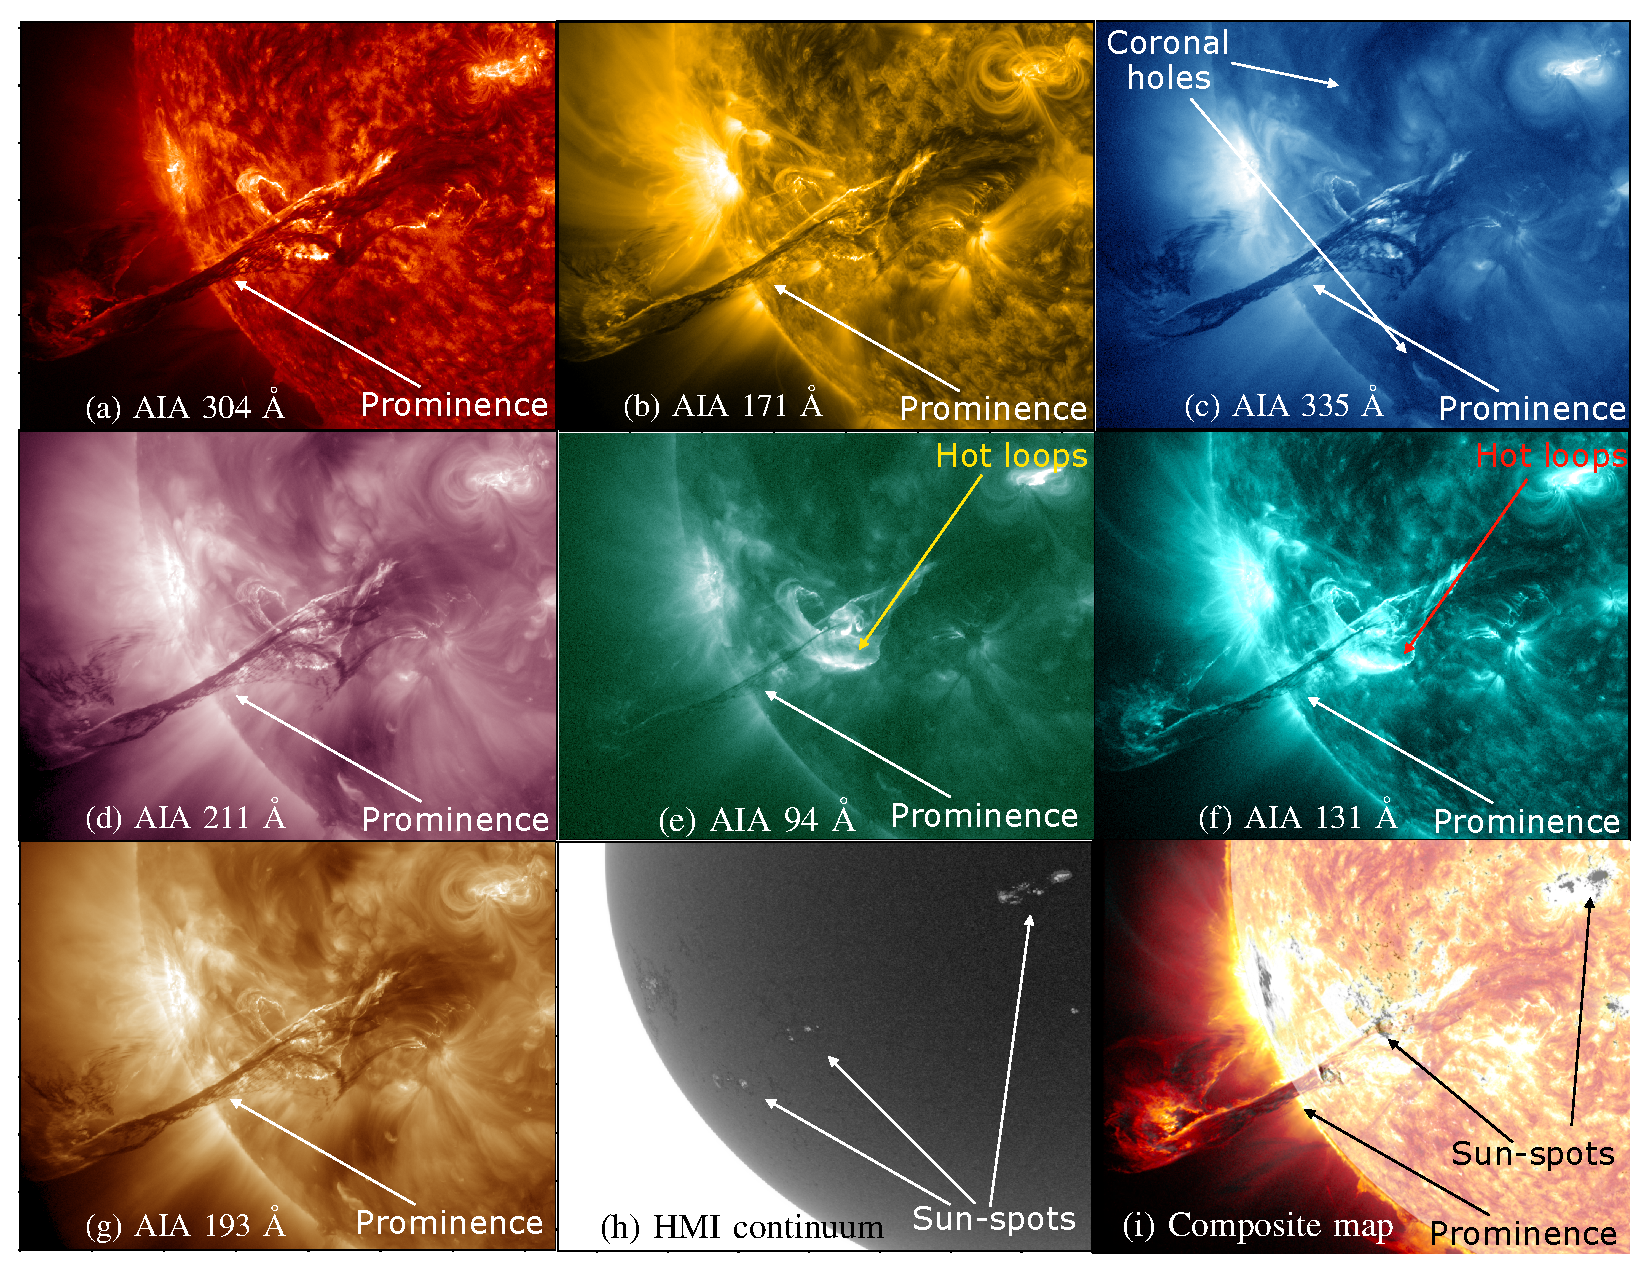
\includegraphics[width=\textwidth]{Figures/aia_features.pdf}
    \caption[Different parts of a flare eruption observed across various wavelengths]{AIA observations of prominence eruption and associated flare as observed on Aug 31st, 2012$\sim$19:50 UT. Different features across different wavelengths have been labelled.}
    %\caption[Different parts of a flare eruption observed across various wavelengths.]{Image of the prominence eruption and associated flare from NOAA AR 11562 on Aug 31st, 2012$\sim$19:50 UT. The prominence is visible in all of the AIA channels. We see the coronal holes in AIA 335 \AA~\textbf{(panel c)}. The flare loops of the associated event is visible in AIA 94 \AA~\textbf{(panel e)} and AIA 131 \AA~\textbf{(panel f)}. The Sunspots are visible in HMI continuum \textbf{panel (h)}. We show a co aligned map of AIA 304 \AA, HMI magnetogram and AIA 131 \AA~in \textbf{panel (i)}. The spatial association of the Sunspots with the hot flareloop plasma and the prominence eruption is clearly demonstrated here. }
    \label{fig:aia-feature}
\end{figure}
%%%%%%%%%%%%%

%\info{I would write the caption of Fig.~\ref{fig:aia-feature} as: AIA observations of prominence eruption and associated flare as observed on Aug 31st, 2012$\sim$19:50 UT. Different features have been labelled.}


%%%%%%%%%%%%%%%%%%%%%%%%%%%%%%%%%%%%%%%%%%%%
\section{Solar Flares}\label{sol_flr}
%%%%%%%%%%%%%%%%%%%%%%%%%%%%%%%%%%%%%%%%%%%%

Solar flares are the most powerful energetic explosions in the Solar system. They are described as a sudden increase in brightness in localized areas of the Sun. Within tens of minutes, they can release over $10^{32}$ erg of energy, which is emitted across the entire electromagnetic spectrum, i.e., from radio to gamma rays. They can also launch highly energetic particles into the interplanetary medium. Flares occur in magnetic active regions. It has been estimated that the amount of flare energy released is comparable to the free energy stored in the magnetic system \citep{emslie12,ash17}. %The term "flare" is generally used explicitly for the entire magnetically-driven event's electromagnetic radiation, as it is the most significant fraction of the total energy liberated. 
The total energy released varies from event to event. It is also known that larger events occur much less frequently than smaller events.

Fig.~\ref{fig:sji_features} displays one of the most well-known and well-studied Solar eruptions from Aug 31st, 2012. During this event, an associated giant prominence erupted from the southeast limb, which was visible in all AIA channels as shown in Fig.~\ref{fig:aia-feature}. The sunspots were also clearly visible and labelled in the HMI continuum (see Fig.~\ref{fig:aia-feature}h). In Fig.~\ref{fig:aia-feature}i, we show the co-aligned AIA 304 {\AA} and HMI continuum observation. The Sunspots lie at the base of the erupted prominence, accompanied by the hot thermal plasma associated with the accompanying flare (visible in Fig.~\ref{fig:aia-feature}e {--} f). The novelty of such observation lies in the clear spatial connection across various layers of the Sun, connected via energy and momentum transported from one layer to the other.

%------------------------------------
\subsection{Brief history of flare observation}\label{sol_flr_1}
%------------------------------------

On September 1, 1859, R.C. Carrington and R. Hodgson independently observed the first flare in white-light continuum~\citep{carrington1859,hodgson1859}. Such localized brightening on the Sun has remained an enigma ever since. 
Shortly after the observation by Carrington and Hodgson, the Sun was being studied extensively in the H$\alpha$ wavelength, which essentially images the chromosphere, and the reports of flaring events became increasingly frequent and progressively more complex. No two events were similar, as there were variations observed in the size of the source, ejections of plasma, and shock waves driving into the interplanetary space. Advances in radio technology during the Second World War affirmed the detection of the presence of non-thermal electrons in the Solar corona during military radar operations \citep{hey46}. Around the same time, S.E. Forbrush noticed ground-level cosmic ray enhancement during major Solar flares. These discoveries eluded that the flaring events do not only involve the thermal plasma but somehow connect with high energy particles and involve the corona. 

In the late 1950s, using rockets and balloons, the Sun was observed with hard X-rays ($\ge~10~keV$). \cite{peterson59} discovered the first hard X-ray emission during a flare in 1958. Later on, it was deduced from the enhancements observed in radio and hard X-rays that the ejected energetic particles may contain a substantial fraction of the initial energy released \citep{brown71}. Note that while the hard X-ray is created by the bremsstrahlung radiation of the electrons colliding into dense material, resulting in a power-law energy distribution, the broadband radio emission from 1 to 100 GHz is created from gyrosynchrotron emission. Flares are now routinely observed with different space-borne instruments, in particular in the EUV and soft X-ray($\le$~10~keV), which shows that the energy released from the flare heats the local plasma to temperatures beyond 30~MK.

%% ################################################################# %%
%\subsection{Neupert effect}\label{npt_eff} \info{I would not give it a name of new subsection}
%% ################################################################# %%

\cite{neupert68} observed a curious correlation that the soft X-ray flux during the rising phase of the flare is proportional to the time integral of the centimetre radio flux since the start of the flare, suggesting a correlation between thermal plasma and the energetic electrons. Note that the centimetre radio flux is emitted by relativistic electrons. A similar correlation was found between the hard X-ray and soft X-ray flux later on. Such correlation can be expressed as,

%%%%%%%%%%%%%%%%%%%%%%%%%%%%%%%%
\begin{equation}\label{npt_eff_eq}
    F_{SXR}(t)~\propto~\int_{t_{0}}^{t}~F_{HXR}(t')~dt'
\end{equation}
%%%%%%%%%%%%%%%%%%%%%%%%%%%%%%%%

\noindent and is known as the ``Neupert effect''. This relationship shows that the soft X-ray radiation primarily originates from a thermal plasma which is heated by the energy of the flaring event deposited by the accelerated electrons. We note, however, that Eqn.\ref{npt_eff_eq} is only valid if cooling by conduction is negligible and/or the role of ions in the flare energy deposition is minimal \citep{veronig05}.

%% ################################################################# %%
\subsection{``Standard'' model of Solar flare}\label{sol_flr_std_mod}
%% ################################################################# %%

Based on various multi-wavelength studies of Solar flares, combined with theoretical modelling a `standard' model of Solar flares has been advocated by \cite{carmichael64,sturrock66,hirayama74,kopp76}, and termed as \textsl{CSHKP} model. The flares occur due to the abrupt release of magnetic free energy, which was previously stored in the coronal magnetic field via flux emergence and surface motions \citep{forbes06}. The majority of the strongest flares are eruptive in nature. The `standard' model attributes the release of flare energy to magnetic reconnection in the corona, which happens due to the eruption and/or coronal mass ejection \citep{shibata95,lin_n_forbes00,moore01,priest_n_forbes02}. It is noteworthy that, despite continuous attempts over the decades, this is not at all a quantitative model. Rather, it is an attempt to unify the multi-wavelength observations and modelling attempts in an orderly manner. Naturally, the model can not explain all the observations from various flares. A schematic picture of the model is shown in Fig.~\ref{fig:std_mod}. Below we describe the salient points of the `standard' model:

%%%%%%%%%%%%%%%%%%%%%%%%%%%%%%%%%%
\begin{figure}[ht!]
    \centering
    \hspace{5cm}
    \includegraphics[trim={1cm 8cm 0cm 8cm}, clip, width=0.95\linewidth]{Figures/std_mod.pdf}
    \caption{A schematic diagram of the standard model of Solar flare.}
    \label{fig:std_mod}
\end{figure}
%%%%%%%%%%%%%%%%%%%%%%%%%%%%%%%%%%

%%%%%%%%%%%%%%%%%

%\info{This whole description of Standard Model needs to be rewritten. You are going too lateral. Here, the aim is not to bring out the caveats, etc, but to outline the standard model. As you say that you are giving the salient features... so just provide that! Not more than 2-3 sentences in each bullet.}

%\begin{enumerate}
    %\item In the standard model, following the reconnection event occurring that releases the magnetic free energy, electrons and ions from the reconnection site are accelerated along the realigned magnetic field lines. The accelerated particles that escape along the open \info{field lines do not open during flares! Please read Aly and Sturocck paper on this! Very interesting concept!} field lines towards the Earth give rise to the particle events seen from Earth \info{which particles are you talking about? There are different kinds of particles -- particles accelerated due to shock waves that come very fast ... remember proton showers on the detector and other particles which are frozen in the field... they come later}. The coronal reconnection source where the energy is released is often observed in HXR. The loop-top HXR \info{are these same as the reconnection source?} sources are often accompanied by the thermal SXR sources. The loop top HXR source is observed above the coronal SXR source \citep{masuda94}. Later on, most of the HXR sources were reported to be cospatial with the SXR source \citep{bataglia_n_benz07}. This thermal source is distinctly different from the post-flare SXR and EUV loops. This thermal coronal source appears before the HXR emission begins, completely contrary to the "Neupert" behaviour. This SXR loop top source is a key behaviour of the pre-flare phase. The emission measure of these sources is higher than typical coronal levels, suggesting evaporation from the chromosphere before the HXR emission. This also suggests that during the early phases of a flare, the energy is conducted gradually by thermal particles, compared to the energetic non-thermal particles later on.
    
    %Given the existence of the thermal source, the coronal non-thermal source can be explained by a beam of non-thermal particles injected into the dense coronal thermal source. Some of the injected electrons escape the coronal source and precipitate lower. This model is known as the intermediate thin-thick target model (ITTT, proposed by \cite{wheatland95} and investigated further by \cite{metclaf99,fletcher98}.) While the ITTT model explains most of the observations from flares there are certain inconsistencies regarding the coronal X-ray source {\it e.g.} the source of coronal SXR in preflare conditions, difference in expected HXR brightness of the cornal source from models to observations still elude us. It is fair to summarise that even though we by and large understand under what ambient conditions how the coronal HXR source is created, we do not understand what underlying process cause such an environment to arise.
    
    %\item The precipitated particles move along the field lines downwards along the magnetic field lines, giving rise to the microwave and radio observations seen from flares via gyro magnetic radiation at various frequencies dictated by the characteristics of local plasma.
    
    %\item The accelerated particles hit the chromosphere, which is considerably denser than the corona, giving rise to Hard X-ray and gamma-ray observed from the foot points. This also explains why the coronal hard X-ray source is considerably softer than the foot points. The energetic particles deposit their energy into the local chromosphere as they go through a series of collisions and eventually thermalize \citep{brown83}. \sroy{Foot point sources are occasionally detected on H-alpha flare ribbons that are approximately 30,000 km apart, marking the base of a magnetic arcade \citep{masuda01}.}

    %\sroy{$\gamma$-ray emission is visible between 0.8 {--} 20 MeV generated by the accelerated ions. The neutron capture line at 2.2 MeV forming Deuterium is usually the strongest characteristic line visible from such emissions. Protons and other accelerated ions collide with the dense chromosphere and produce neutrons. These neutrons are captured by ambient protons to form Deuteron \citep{ramtay74,hua87}. There were later RHESSI observations \citep{hurford_2003,hurford_2006} that showed that the $\gamma$-ray footpoints did not coincide with the HXR footpoints. This demonstrated that the ions and electrons were accelerated differently, as proposed by \cite{emslie_2004}.}
    %\item  As the plasma thermalizes, it emits in thermal bremsstrahlung, giving rise to the soft X-ray \sroy{radiation}. Also, as the energy is deposited into the chromosphere from the accelerated particles, it heats the local chromosphere environment it gradually increases the local pressure. As the pressure grows, when the pressure gradient builds up enough, the local plasma starts expanding upwards(essentially due to buoyancy) and slowly fills up the coronal loops with soft X-ray emitting plasma. This phenomenon is known as "Chromospheric evaporation". This was directly observed in blue-shifted lines of hot material. \sroy{This was first reported by \cite{doscheck80,feldman80}. \cite{antonucci89} reported velocities of 300 {--} 400 km/s with temperature $\sim$ 20 MK in \ion{Ca}{19}, while later on \cite{milligan06} reported much gentler up-flow with velocities $\sim$ 200 km/s in \ion{Fe}{19} line from {\it SOHO}/CDS observations. Several simulations also reproduced evaporation arising from non-thermal particle precipitation \citep{sterling93,hori98,reeves07}.}
    %\item This whole scenario explains the Neupert effect. As the energy form the accelerated particles is converted into the soft X-ray emitting plasma, and it builds up over time. That explains the soft X-ray being proportional to the time integral of the hard X-ray flux.
%\end{enumerate}
%%%%%%%%%%%%%%%%%

%%%%%%%%%%%%%%%%%
\begin{enumerate}
    \item In the standard model, following the reconnection event occurring that releases the magnetic free energy, electrons and ions from the reconnection site are accelerated along the realigned magnetic field lines downwards. In the case of an associated CME, parts of the magnetic energy is deposited as kinetic energy. The coronal reconnection source where the energy is released is often observed in HXR. The loop-top HXR sources are often accompanied by the thermal SXR sources. The loop top HXR source is observed above the coronal SXR source \citep{masuda94}.
    
    \item The precipitated particles move along the field lines downwards along the magnetic field lines, giving rise to the microwave and radio observations seen from flares via gyro magnetic radiation at various frequencies dictated by the characteristics of local plasma.
    
    \item The accelerated particles hit the chromosphere, which is considerably denser than the corona, giving rise to Hard X-rays and gamma-rays observed from the foot points. This also explains why the coronal hard X-ray source is considerably softer than the foot points. The energetic particles deposit their energy into the local chromosphere as they go through a series of collisions and eventually thermalize \citep{brown83}. Foot point sources are occasionally detected on H-alpha flare ribbons that are approximately 30,000 km apart, marking the base of a magnetic arcade \citep{masuda01}.

    \item $\gamma$-ray emission is visible between 0.8 {--} 20 MeV generated by the accelerated ions. The neutron capture line at 2.2 MeV forming Deuterium is usually the strongest characteristic line visible from such emissions. Protons and other accelerated ions collide with the dense chromosphere and produce neutrons. These neutrons are captured by ambient protons to form Deuteron \citep{ramtay74,hua87}. There were later RHESSI observations \citep{hurford_2003,hurford_2006} that showed that the $\gamma$-ray foot-points did not coincide with the HXR foot-points. This demonstrated that the ions and electrons were accelerated differently, as proposed by \cite{emslie_2004}.

    \item  The thermalized plasma emits in thermal bremsstrahlung, giving rise to soft X-ray and EUV radiation. The heating of the local chromosphere gradually increases the local pressure. When the growing pressure gradient builds up enough, the local plasma starts expanding upwards and slowly fills up the coronal loops with soft X-ray-emitting plasma. This phenomenon is known as "Chromospheric evaporation". This was first reported by \cite{doscheck80,feldman80}. \cite{antonucci89} reported velocities of 300 {--} 400 km/s with temperature $\sim$ 20 MK in \ion{Ca}{19}, while later on \cite{milligan06} reported much gentler up-flow with velocities $\sim$ 200 km/s in \ion{Fe}{19} line from {\it SOHO}/CDS observations. Several simulations also reproduced evaporation arising from non-thermal particle precipitation \citep{sterling93,hori98,reeves07}.
\end{enumerate}
%%%%%%%%%%%%%%%%%

It is important to emphasise that while the standard model attempts to explain and unify various kinds of differences seen from the numerous flares we observe, there are several cases where the standard model cannot explain the observations. For example, there have been observations of flares where the hard X-ray footpoint does not form. It is proposed that in these cases, the plasma in the coronal loops is so dense that the accelerated particles pass through enough collisions to thermalize within the flare loops before reaching the chromosphere. In this process, they may defuse the energy more evenly within the loop rather than impulsively dumping it at the base of the loops \citep{veronig02,veronig04}. Another flare which previously occurred at the same region might explain the denser coronal loops \citep{strong84,bone07}.  

%% ################################################################# %%
\subsection{The energetics of Solar flares}\label{sol_flr_energ}
%% ################################################################# %%

Given the rich history of flare observations over more than 150 years, remarkably enough, we have barely started scratching the surface of the complexities involved in the physics of Solar flares. The reconfiguration of the magnetic structures, which almost always involves complex geometry, makes almost all events unique in some sense. Following the reconfiguration of the magnetic field, the released magnetic free energy is transported across various layers of the Sun and converted into various other forms of energy. The overarching conversion of magnetic energy into various forms, i.e., reconnection outflow, particle acceleration, thermal and kinetic energy of chromospheric plasma, etc, has proven incredibly complex to model. In cases where flares are associated with eruptions, e.g., CMEs, there is the added complexity of the kinetic and potential energy of the CMEs, the associated shocks and the kinetic energy of the Solar energetic particles.
%Considering how the energy is transformed the magnetic energy of the active region that is released after the reconnection into the reconnection outflow jets, the kinetic energy of escaping particles, the thermal and the kinetic energy of the Chromospheric plasma evaporating, the radiative and conductive losses. In case of the eruptive events, there is the added complexity of the kinetic and potential energy of the CMEs, the energy of the shocks and the kinetic energy of the solar energetic particles. 

To constrain the models of Solar flares and the various associated phenomena, detailed quantitative characterization is absolutely necessary. %There have been several studies quantifying the partition between various subsets of the energies. 
The questions which are of particular importance are:

%%%%%%%%%%%%%%%%%%%%%%%%%%%%%%%%%%%%%%%%%%%%%
\begin{itemize}
    \item Do active regions have enough free energy to account for the total energy released in the solar flares and their associated phenomena?
    \item What is the energy partition between flares and CMEs?
    \item Do the non-thermal component of flares have enough energy to completely power the thermal component or an extra energy source is required to power the thermal component?
\end{itemize}
%%%%%%%%%%%%%%%%%%%%%%%%%%%%%%%%%%%%%%%%%%%%%


%%%%%%%%%%%%%%%%%%%%%%%%%%%%%%%%%%%%%%%%%%%%%
%\begin{itemize}
%    \item \textbf{If an active region can have enough free energy to account for the total energy released in the solar flares and/or CMEs.}
%    \item \textbf{What is the energy partition between flares and CMEs.}
%    \item \textbf{If the non-thermal component have enough energy to power up the thermal component.}
%\end{itemize}
%%%%%%%%%%%%%%%%%%%%%%%%%%%%%%%%%%%%%%%%%%%%%

While it is now established the active regions have enough magnetic free energy to power the flare and CME and other associated phenomena  \citep{emslie12,ash17}, the energy partition between the flare and associated CME is much more fuzzy. \cite{emslie12} found that the flare and CME have energies of the same order of magnitude, while \cite{ash17} concluded the energy in the flare dominates that of the associated CME. 

The question about the non-thermal component having sufficient energy to power the thermal component is still unresolved, as even the most recent studies contradict each other in the most puzzling fashion. \cite{warmuth20} discussed the contradictions arising from some of the studies~\citep{stosire07,emslie12,inglis14,warmuth16a,warmuth16b,ash17}, the details of which are summarized in Table~\ref{tab1}.

%%%%%%%%%%%%%%%%%%%%%%%%%%%%%%%%%%%%%%%%%%%%%%%
\begin{table}[ht!]
    \centering
    \resizebox{\textwidth}{!}{%
    \begin{tabular}{||c|c|c|c|c|c|c||}
    \hline 
    \hline
       Study & No. of flares & GOES class range & Thermal model & Thermal spectrum & Thermal volume & Thermal losses \\
       \cite{stosire07} (S07 from hereon) & 18 & A3-B7 & Isotherm. & RHESSI & TRACE & X \\
       \cite{emslie12} (E12 from hereon) & 38 & C5-X28 & Isotherm. & RHESSI & RHESSI & Rad. \\
       \cite{inglis14} (IC14 from hereon) & 10 & B3-B9 & Multitherm. & RHESSI+AIA & RHESSI & Rad. \\
       \cite{warmuth16a,warmuth16b} (WM16 from here on) & 24 & C3-X17 & Isotherm. & RHESSI+GOES & RHESSI & Rad.,Cond. \\
       \cite{ash17} (A17 from here on) & 188 & M1-X7 & Multitherm. & AIA & AIA & Rad. \\
       \hline
    \end{tabular}}
    \caption{Observational summary of the flares as described in \cite{warmuth20}.}
    \label{tab1}
\end{table}
%%%%%%%%%%%%%%%%%%%%%%%%%%%%%%%%%%%%%%%%%%%%%%%

The bolometric energy serves as a representation of the overall energy released during solar flares. Regardless of the mechanism of energy release, e.g., through direct plasma heating, rapid bulk flows, or non-thermal particles, etc., the ultimate outcome is the thermalization of the plasma and the subsequent radiation. Since the bolometric energy encompasses the entire electromagnetic spectrum, it reflects the total energy originally of the flare. Note, however, that this bolometric energy only pertains to the energy liberated within the flare and does not include the energy associated with the concurrent CME. %\cite{warmuth20} used the bolometric energy released in solar flares to compare various studies on equal footing. Here we will discuss some of the main issues \cite{warmuth20} identifies comparing these studies.

Fig.~\ref{fig:goes-therm} displays correlation plots between peak thermal energy and peak GOES flux (left panel) for various flares studied by various authors and corresponding (where available) volume estimates of the thermal plasma (right panel). The plots show that the estimated thermal energy obtained in all studies shows an excellent correlation with peak {\it GOES} flux. Also plotted are the bolometric energies obtained by \cite{emslie12, kretzschmar11}. %Fig.~\ref{fig:goes-therm} left panel shows the peak thermal energy as a function of peak {\it GOES} flux for all the flares from the five studies. 
Note that the thermal energy obtained by E12 (open red diamonds) and WM16 (filled black circles) are consistently one order of magnitude lower than the bolometric energy (open green diamonds and solid green line) of flares with similar peak GOES flux. Extrapolation of E12 and WM16 is about half an order of magnitude lower compared to IC14 (open blue triangles), while S07 (open pink flipped triangles) is very consistent with the extrapolation. Note that the energies estimated in A17 (orange plus signs) are about an order of magnitude higher than that obtained in other studies and even higher than the extrapolated bolometric energy for flares of the same class from \cite{kretzschmar11} and E12. These results present a contradiction in the results obtained in different studies. While there could be several reasons for these differences, they can be attributed to differences in modelling the thermal component of the flares. For example, {\it RHESSI} usually yields a higher temperature and lower emission measure compared to {\it GOES} due to the highly multi-thermal nature of the flaring plasma \citep{bataglia05,ryan14,warmuth16a}. Although the {\it GOES} temperature is higher by a factor of 1.4, it is not dependent on the flare class. Moreover, \cite{warmuth20} also investigated whether assuming an isothermal or multi-thermal model introduces any differences in the thermal energy estimates. They reported no significant differences due to differences in models (refer to Fig.2 and the corresponding discussion in \cite{warmuth20}). Notably, these comparisons of isothermal and models are made by fitting spectra obtained by spatially binning spectra. This does not really incorporate the multithermal nature of the plasma varying spatially.

%%%%%%%%%%%%%%%%%%%%%%%%%%%%%%%%%%%%%%%%%%%%%%%
\begin{figure}[ht!]
    \centering
    \includegraphics[width=0.49\textwidth,trim={0cm 0cm 0cm 0.02cm},clip]{goes_flux_therm.jpg}
    \includegraphics[width=0.49\textwidth,trim={0cm 0cm 0cm 0.02cm},clip]{goes_flux_vol.jpg}
    \caption[Correlation of peak {\it GOES} flux with peak thermal energy and flaring plasma volume.]{{\it GOES} peak thermal energy (left panel) and volume of the thermal plasma (right panel) as a function of the peak {\it GOES} flux for all the flares from five studies (figure credit: \cite{warmuth20}). The C values show the linear correlation coefficient for various studies.}
    \label{fig:goes-therm}
\end{figure}
%%%%%%%%%%%%%%%%%%%%%%%%%%%%%%%%%%%%%%%%%%%%%%%

The thermal energy estimated usually depends on the source volume, $\mathrm{U_{Th}\sim n_{e}k_{B}TVf}$. Fig.~\ref{fig:goes-therm} right panel shows the volumes used for various studies to estimate the thermal energy as a function of the peak {\it GOES} flux. Apart from S07 and A17, all other studies used {\it RHESSI} imaging to estimate the flare volume with a filling factor $f=1$. S07 determined the volume by employing a semicircular loop model, utilizing the cross-sectional area and loop length derived from the observed areas and separations of foot point brightening of 1600  {\AA} by {\it TRACE}. In contrast, A17 estimated the volume based on the flare area exceeding a certain threshold in the emission measure obtained from the spatial synthesis DEM method. 

It is worth noting that the volume estimates from E12 and WM16 align closely, as do those from A+17, despite employing entirely different methodologies. In contrast, the micro flare volumes reported by IC14 are notably larger, ranging from one to two orders of magnitude beyond what would be anticipated based on the findings of the other four studies. Intriguingly, this discrepancy aligns with the additional volume required to account for the higher thermal energies observed in IC14. The uncertainty in detecting volume can be due to the CLEAN (Component Least Squares Deconvolution) algorithm systematically overestimating the source size \citep{warmuth13a}. There have also been studies demonstrating that {\it RHESSI} has difficulties in resolving small sources \citep{dennis09,warmuth13b}, that would be applicable for small thermal sources in the microflares. This illustrates the requirement for better volume estimation for better estimates of the thermal energy of flares.

We can conclude a few more puzzling questions from these studies as a whole: %\info{These are not questions but more like statements. Please make them questions.}

%--------------------------------------------------------------------
\begin{itemize}
    \item The primary challenge in estimating the thermal energy of the hot plasma stems from determining the temperature distribution of the plasma using Differential Emission Measure (DEM), and the radiating plasma volume. How strongly do the uncertainties of determining the thermal energy depend on the uncertainties of the volume estimation and the highly mutithermal nature of the flaring plasma? 
    \item The dissipation of energy from the hot plasma is substantial. Although there is widespread agreement regarding radiative losses across studies, the extent of conductive losses disagree significantly between the studies. Why do various studies vary so significantly on the extent of conductive losses across the literature and what effect does it have on the thermal evolution of the flares?
    \item How much do the non-thermal energy in injected electrons depend on the poorly constrained low-energy cutoff?
    \item The thermal and non-thermal energy partition changes with flare class. In smaller flares, there appears to be a deficiency of energetic electrons, whereas in larger flares, the injected non-thermal energy seems to be sufficient in powering the thermal component. Does this signify the existence of an additional third heating source?
\end{itemize}
%--------------------------------------------------------------------

In the limited scope of this thesis we can only address some aspects of these persisting questions. Here we briefly outline these questions:
%--------------------------------------------------------------------
\begin{itemize}
\item How does the thermal and non-thermal energy partition change over the duration of flares? What effect do the uncertainties of volume estimation have, on the thermal energy estimates and what conclusions can we draw from that regarding the tension in the thermal and non-thermal energy sources?
\item Flares connect various layers of the solar atmosphere via different mechanisms during various stages of its evolution. How does the signature of flares look in the NUV regime which mainly originate in the photosphere, chromosphere and transition region. The transition region is one of the least observed part of the solar atmosphere in context of flares. What is the spectral energy distribution of flares across various wavelength regime and layers, specifically in NUV?
\end{itemize}
%--------------------------------------------------------------------

%\info{I would also suggest that you use this section to identifiy all the questions that you are going address in the thesis... partition between thermal and non-thermal is one, other is NUV radiation in flare etc...}

%In addition to these, there is one more looming question, related to the "standard" model of flares itself, that has been largely unanswered, not due to lack of efforts, rather limited mostly by the technological limitations dictating the detectability of the current instruments. In \S\ref{sol_flr_std_mod}, we discussed about the fundamental differences inferred between the acceleration mechanisms of electrons and ions inferred from the different locations of the HXR and $\gamma$-ray foot points. The production of $\gamma$-ray from nuclear reactions in chromosphere opens up the possibility of high-energy nuclear reactions producing pions ($\pi^{0}$ and $\pi^{\pm}$) along with secondary neutrinos ($\nu$) through the decay of the pions. Such reactions would be driven by protons with energy $>$ 300 MeV \citep{ramtay75,hudson_n_ryan_95}. Detection of neutrinos will open up a new window in constraining the effects of the accelerated particles in the lower solar atmosphere, i.e., chromosphere and photosphere and the general characteristics of the local plasma environment. Unfortunately, in spite of considerable efforts no flare neutrinos have been detected so far. It is understood that the first hurdle is to detect a minute transient signal on top of the large solar neutrino background. This informs our required detection thresholds driven by the current ion acceleration models \citep{sol_nu_kamiokande,abe_2022}. If the inability to detect flare neutrinos persists, it indicates that not enough protons/ions with energies $>$ 300 MeV is produced even in very large flares. That would impose an upper limit of the amount of energy that is deposited in particle acceleration from flaring events and/or the efficiency of the acceleration mechanism. \info{this discussion is good here but not necessary. I leave it to you to decide!}

%--------------------------------------------------------------------
\section{Motivation}\label{sec:mot}
%--------------------------------------------------------------------
%\info{This section is what we shall use as the synopsis. So, it should have : 1 st para: What are flares and why are they important. 2nd para: what is know and what is missing (only the most important aspects). 3rd Para: what is the overall goal, and what extra do you do? Just briefly. Thereafter Chapter wise summary.}

%The main motivation of this thesis is to add understanding of effects of flares on the surrounding environment in lower and upper solar atmosphere, to answer some of the questions posed above. We have used imaging and spectroscopic observations from multiple space based observatories, e.g., AIA, HMI, IRIS, XRT, etc. This research contributes to creating a perspective of flare energetics and its effect on the surrounding plasma environment from chromosphere to corona. \info{again written with Capital C...}

The solar flares are the strongest magnetic event in our solar system connecting various layers of the solar atmosphere ({\it e.g.} from photosphere to corona), coupled via mass and energy transport. While the coronal manifestation of solar flares has been studied extensively with several instruments, there are only a few imaging and spectroscopic instruments observing the photosphere to transition region. These include the {\it IRIS} \citep{iris}, AIA 1600, 1700, and 304~{\AA} \citep{aia} and some other filters of {\it Hinode}/SOT \citep{sot}. In addition to these, we also have had balloon experiment {\it SunRISE} \citep{Sunrise1,Sunrise2}, which provided high-resolution imaging of the chromosphere, from the SuFI instrument \citep{sufi}.

This illustrates the necessity of more observatories operating at the chromospheric wavelengths for a more comprehensive understanding of how the solar flares manifest and affect the dynamics and heating of the lower solar atmosphere. More specifically, there is a gap in understanding the spectral energy distribution of flares and the flare signatures in NUV arising from the chromosphere and photosphere. 

The main motivation of this thesis is to add an understanding of the effects of flares on the surrounding environment in the lower and upper solar atmosphere to answer some of the questions posed in \S\ref{sol_flr_energ}. We have used imaging and spectroscopic observations from multiple space-based observatories, e.g., AIA, HMI, IRIS, XRT, etc. This research contributes to creating a perspective of flare energetics and its effect on the surrounding plasma environment from the chromosphere to the corona.

%\info{Shouldn't the above two paragraphs swapped?}


%This illustrates the necessity of more observatories operating at the transition region \info{There is a lot of upper transition region data e.g., 171, what is missing is chromosphere. SUIT does not observe transition region} wavelengths for more comprehensive understanding about how the solar flares manifest and affect the dynamics and heating of the lower solar atmosphere. In this regard, {\suit} onboard Aditya-L1 will play a crucial role in probing the lower solar atmosphere. The various imaging channels of {\suit} would observe the manifestation of flares in transition region at various heights (NB3 $\implies$ \ion{Mg}{2} k 279.6 nm, NB4 $\implies$ \ion{Mg}{2} h 280.3 nm, NB8 $\implies$ \ion{Ca}{2} h 396.8 nm), further lower in the transition region (NB2 $\implies$ blue wing of Mg window, NB5 $\implies$ red wing of Mg window) and Sunspots and possible signature of umbral brightening due to flares at the photosphere (NB6 300 nm and NB7 388 nm) in full disk. This would also allow us to probe the interaction of the flaring region, with other active regions on disk, giving us a comprehensive overview of the effect of solar flares and their manifestation in the lower solar atmosphere.

%% ################################################################# %%
\section{Outline of Thesis}\label{sec:outline}
%% ################################################################# %%

The work within this thesis spans across various layers of the solar atmosphere to understand how solar flare couples these layers. It is carried out partly, as various preparatory analysis for {\suit}, forward modelling {\suit} observations, designing the stellar calibration scheme for {\suit}, analysis of existing transition region observations in anticipation of {\suit} observations, analysis of coronal observations of solar flares, and analysis of first solar flare observations by {\suit}. Here, I will briefly discuss the structure of the rest of the thesis: 

%%%%%%%%%%%%%%%%%%%%%%%%%%%
\begin{itemize}

    \item In chapter \ref{c:chap2}, we review various space based missions and their respective payloads which are used in this thesis. We discuss various analysis techniques used in this thesis. We also motivate the importance of {\suit} and its main science goals. In addition, we briefly discuss the specific questions regarding solar flares we can address with {\suit}.

    \item We address the issues raised in \S\ref{sol_flr_std_mod} regarding the uncertainties of volume estimation for flaring plasma and its effects on the thermal energy estimation in chapter \ref{c:chap3}. We use observations from {\it SDO}/AIA, {\it STEREO-A}/EUVI, {\it SO}/STIX, {\it GOES}/SUVI to estimate the thermal energy of two solar flares. We propose a method using existing tools, to use observations from different vantages ({\it e.g.} AIA and EUVI from different angles) to accurately calculate the volume of the flare arcade and estimate the thermal energy. We show that the accurate estimate as a function of time can have effects on the accurate estimation of thermal energy and the partition between the thermal and non-thermal component.

    \item In chapter \ref{c:chap4}, we discuss the forward modelling pipeline developed for {\suit}. We use MPS-Atlas simulation and {\it IRIS} observations, with measured transmission profiles of various optical components and the PSF to forward model {\suit} observations. We also discuss a preliminary version of the deconvolution algorithm that will be deployed in the data reduction pipeline.

    \item In chapter \ref{c:chap5}, we discussed some of the initial preparatory analysis we did for {\suit}, including the throughput model for {\suit}, how the filters mounted on {\suit} were chosen, the analysis of spacecraft jitter simulation and what effect it would have on the imaging. We also describe the stellar calibration scheme and the selection criteria for the standard star target. We use a Sun-as-a-star spectra to evaluate the calibration scheme with the aforementioned throughput model.
    
    \item In chapter \ref{c:chap6}, we use existing {\it IRIS} observations of three solar flares to probe how the lower solar atmosphere is affected by the flares. The ratio of the \ion{Mg}{2} k and h lines, is a proxy for the optical depth of the surrounding plasma. Hence, we use the observations of \ion{Mg}{2} lines along HMI magnetic field measurements to investigate the effects of magnetic field, if any. \cite{kerr15} conducted a similar study and found signatures of localised heating in the line intensity ratio. We found, that the line intensity ratio shows a correlated increase and decrease with the flare light curve. We argue this to be signature of plasma flow associated with flare, and a change in density of the local environment. This acts as a prelude of what is achievable with {\suit}. We can use a similar method to give full disk context of optical depth, with respect to eruptive events.

    \item In Chapter \ref{c:chap7}, we discuss some of the first flares observed by {\suit}. First, we report the observation of the limb event on 31st December 2023. We see an ejection of a plasma blob from the flaring active region in the NB4 (Mg \Romannum{2} h) pass-band. We find that the plasma blob aligned with the bright parts of the ejected loops, as observed from AIA. From a DEM analysis we find that the region is denser and cooler compared to the rest of the ejected loop structure. Further, we find that the velocity of the ejected plasma is consistent with the observations from AIA 1600 {\AA}. The velocity shows a rapid acceleration, which is co-temporal with the development of a kink in the 1600 {\AA} loops. The HXR lightcurve is also indicative of ongoing bursty reconnection during this time. We believe a bursty reconnection associated with the ejection of chromospheric material can explain the {\suit} observations.

    Next, we discuss the observations of the X-class flare on 22nd February 2024 in chapter 8. The flare was associated with penumbral bright kernels observed in NB2 (blue wing of Mg \Romannum{2} window) and NB5 (red wing of Mg \Romannum{2} window). The kernels were also observed in HMI WL observations. Similar observations were made by \cite{kowalski19} with SJI 2832 {\AA} for a different event. They attributed the bright kernels to various photospheric metallic lines going into emission. They demonstrated this could be possible due to the electron beam's localised heating in the photosphere. We use {\it Chandrayan-2}/XSM observations to show that the appearance of bright kernels does not align with the HXR peak observed from STIX but rather with the photospheric Fe line fluorescence. We show the appearance of these photospheric metal lines can also be explained via Fe line fluorescence.
    
    \item Finally in Chapter \ref{c:chap8} we present a summary of the results obtained in the various projects in context of the overarching perspective of flare energetics and its signature in the chromosphere and photosphere in NUV. We also discuss the caveats, the eventual progression of these projects and what new questions they open up. Moreover, we also discuss the likely required observations to address the questions regarding flares and which questions they would address.
   % \item In chapter \ref{c:chap7} we discuss the first flare observations of {\suit}. What do you find? 
\end{itemize}


%\listoftodos
%%%%%%%%%%%%%%%%%%%%%%%%%%%
\clearpage
%
\chapter{Existing Solar Observations and Techniques: A bridge towards Solar Ultraviolet Imaging Telescope}\label{c:chap2}
\chaptermark{Solar Observatories and Analysis Techniques}
%UNLIKE IN A REGULAR TEX FILE, DON'T PUT ANY PREAMBLE MATERIAL HERE

%UNLIKE IN A REGULAR TEX FILE, DON'T PUT ANY PREAMBLE MATERIAL HERE

%%%%%%%%%%%%%%%%%%%%%%%%%%%%%%%%%%%%%%%%%%%%
%\section*{Introduction}
%%%%%%%%%%%%%%%%%%%%%%%%%%%%%%%%%%%%%%%%%%%%

\justifying

The remarkable technological progress attained in the last few decades has yielded significant benefits in the form of highly advanced imaging, spectroscopic, and polarimetric instruments designed for astronomical observations. These instruments have empowered us with the ability to scrutinize the Sun with exceptional detail. Specifically, the space based observatories have added new avenues of observing sun. Large portions of the electromagnetic spectra is heavily by Earth's atmosphere \sr{Reference here}.  

The studies within this thesis are using solar observations are multi wavelength analysis of solar flares with both imaging and spectroscopy. In this chapter we describe the details of the instruments and techniques used for our analysis.

%%%%%%%%%%%%%%%%%%%%%%%%%%%%%%%%%%%%%%%%%%%%
\section{Solar Dynamics Observatory}
%%%%%%%%%%%%%%%%%%%%%%%%%%%%%%%%%%%%%%%%%%%%

The Solar Dynamics Observatory \citep[SDO;][]{sdo} is a NASA mission designed to understand the causes of solar variability at various spatio temporal and wavelength scales, as well as its impacts on Earth and the near-Earth environment. It is part of NASA’s Living With a Star program and houses multiple instruments onboard to address its numerous scientific goals. Among the numerous instruments on-board {\it SDO}, we have extensively used data from two instruments – the Atmospheric Imaging Assembly (AIA) and the Helioseismic and Magnetic Imager (HMI).

%%%%%%%%%%%%%%%%%%%%%%%%%%%%%%%%%%%%%%%%%%%%
\subsubsection{Atmospheric Imaging Assembly (AIA)}
%%%%%%%%%%%%%%%%%%%%%%%%%%%%%%%%%%%%%%%%%%%%

AIA \citep{aia} obtains full-disk images of the solar transition region and corona at unprecedented spatio-temporal resolution. The field of view (FOV) covers up to 0.5 $\mathrm{R_{\odot}}$ above the limb. It incorporates several filters at 94 {\AA}, 131 {\AA}, 171 {\AA}, 193 {\AA}, 211 {\AA} and 335 {\AA}, mainly probing the Corona, along with filters at 304 {\AA}, 1600 {\AA}, 1700 {\AA}, and 4500 {\AA}, mainly observing the Chromosphere and Photosphere, providing a total temperature coverage range of 0.06 MK to 20 MK and across various heights. Figure 2.1 illustrates the temperature responses of these filters \citep{borner12}, derived based on the CHIANTI model for solar emissivity \citep{chianti,chianti1}. Under different conditions, these AIA filters observe different plasma phenomena \citep{o'dwyer10}. Typical exposure times range between 0.5 and 3 seconds. Each AIA telescope is accompanied by its own guide telescope to ensure highly accurate image stabilization. For ous analysis, we have extensively used the coronal EUV channel observations from AIA, e.g. 94 {\AA}, 131 {\AA}, 171 {\AA}, 193 {\AA}, 211 {\AA} and 335 {\AA}. These coronal channels observations are usually available with a 12 s cadence.

%%%%%%%%%%%%%%%%%%%%%%%%%%%%%%%%%%%%%%%%%%%%
\subsubsection{Helioseismic and Magnetic Imager (HMI)}
%%%%%%%%%%%%%%%%%%%%%%%%%%%%%%%%%%%%%%%%%%%%

HMI \citep{hmi} obtains images of the Sun across the \ion{Fe}{1} 6173 {\AA} line at six wavelength locations and infers all four components of the Stokes' parameter. Using these observations, various parameters are inferred e.g., Line of Sight (LOS) magnetic field, Doppler velocities, vector magnetic fields etc. We have mainly used the LOS magnetogram for our analysis. These magnetograms have a 0.5{\arcsec} per pixel resolution and 45 s cadence.

%%%%%%%%%%%%%%%%%%%%%%%%%%%%%%%%%%%%%%%%%%%%
\section{Interface Region Imaging Spectrograph (IRIS)}
%%%%%%%%%%%%%%%%%%%%%%%%%%%%%%%%%%%%%%%%%%%%

The Interface Region Imaging Spectrograph \citep[IRIS;][]{iris} is a NASA small satellite explorer mission designed to observe the dynamics of the lower solar atmosphere. IRIS contains a spectrograph and a slit-jaw imager (SJI), observing the chromosphere, the transition region, and the lower corona. It primarily observes the Sun in two pass bands around 1400 {\AA} and 2800 {\AA}. IRIS provides data at high spatial resolution (0.33 {\arcsec} in FUV and 0.4 {\arcsec} in NUV), high time cadence (up to 1 second), and high spectral resolution (12 or 25 m{\AA} per pixel).

IRIS observes three wavelength bands: two in the Far Ultraviolet (FUV) range, spanning 1331.7–1358.4 {\AA} and 1389.0–1407.0 {\AA}, and one in the Near Ultraviolet (NUV) range, covering 2782.7–2851.1 {\AA}. IRIS measures spectra through two primary modes: raster and sit-and-stare. In raster mode, the slit traverses a field of view, capturing spectra from each pixel along its path. When the displacement between consecutive slit positions is comparable to the slit width, it is called dense raster mode; otherwise, it is called sparse raster mode. Alternatively, the instrument may position the slit on a specific region for observation of the Sun. This mode can allow the Sun to naturally rotate across the region or adjust for solar rotation while maintaining continuous observation. This mode is referred to as sit-and-stare. In our analysis, we have used both spectra and SJI imaging from the \ion{Mg}{2} h \& k window and SJI imaging from the \ion{Si}{4} 1402 {\AA} window.

%%%%%%%%%%%%%%%%%%%%%%%%%%%%%%%%%%%%%%%%%%%%
\section{Spectrometer/Telescope for Imaging X-rays (STIX)}
%%%%%%%%%%%%%%%%%%%%%%%%%%%%%%%%%%%%%%%%%%%%

Solar Orbiter \citep[SO;][]{so} is a joint mission between the European Space Agency (ESA) and NASA, launched in February 2020 with the goal of studying the Sun and its dynamic behaviour. The spacecraft aims to provide unprecedented observations of the Sun's polar regions and the inner heliosphere, offering new insights into solar phenomena such as solar wind, coronal mass ejections, and the Sun's magnetic field. We have used observations from the Spectrometer/Telescope for Imaging X-rays (STIX) instrument for our analysis.

 STIX \citep{stix,stix1} is designed to study the Sun's X-ray emissions, providing crucial insights into the processes driving solar flares and other high-energy phenomena. STIX incorporates a set of collimators and detectors to capture high-resolution images of the Sun in X-rays. These images allow scientists to pinpoint the locations and intensities of X-ray emissions associated with solar flares. The instrument covers a broad range of X-ray energies, from approximately 4 to 150 keV, enabling it to observe various aspects of solar activity. STIX can capture X-ray data with high temporal resolution, allowing scientists to study the rapid evolution of solar flares and other transient events in detail. STIX works together with other instruments onboard Solar Orbiter, providing complementary measurements to enhance our understanding of the Sun's dynamic behaviour across different wavelengths and energy ranges.

%%%%%%%%%%%%%%%%%%%%%%%%%%%%%%%%%%%%%%%%%%%%
\section{Extreme Ultraviolet Imager (EUVI)}
%%%%%%%%%%%%%%%%%%%%%%%%%%%%%%%%%%%%%%%%%%%%

Solar Terrestrial Relations Observatory-Ahead \citep[{\it STEREO-A};][]{stereo}, is one of two spacecraft in NASA's STEREO mission, which was launched in October 2006 with the goal of studying the Sun and its dynamic behaviour. {\it STEREO-A} and its twin spacecraft {\it STEREO-B} (Behind) were designed to provide stereoscopic views of the Sun, enabling three-dimensional observations of solar phenomena such as coronal mass ejections (CMEs) and solar flares. Extreme Ultraviolet Imager \citep[{\it EUVI};][]{euvi} is one of the key instruments onboard the {\it STEREO-A} spacecraft. {\it EUVI} is designed to capture images of the Sun in the extreme ultraviolet (EUV) wavelength range. This range of wavelengths is particularly useful for studying the Sun's outer atmosphere, known as the corona, and observing features such as solar flares, coronal loops, and coronal holes. 

{\it EUVI} can capture high-resolution images of the Sun's corona, with spatial resolutions in order of a few arcseconds. It can observe the Sun in 171 {\AA}, 195 {\AA}, 284 {\AA} and 304 {\AA} simultaneously. {\it EUVI} provides continuous observations of the Sun from the STEREO-A spacecraft's vantage point, located slightly ahead of Earth in its orbit around the Sun. This allows {\it EUVI} to monitor solar activity over extended periods and to track the evolution of solar features such as sunspots, flares, and coronal mass ejections (CMEs). We have used 171 {\AA} and 195 {\AA} observations from EUVI for our analysis.

%%%%%%%%%%%%%%%%%%%%%%%%%%%%%%%%%%%%%%%%%%%%
\section{X-Ray Telescope (XRT)}
%%%%%%%%%%%%%%%%%%%%%%%%%%%%%%%%%%%%%%%%%%%%

{\it Hinode} \citep{hinode}, meaning "Sunrise" in Japanese, is a space mission launched by the Japan Aerospace Exploration Agency (JAXA) in collaboration with NASA and the UK Space Agency in September 2006. Also known as Solar-B before its launch, {\it Hinode} is dedicated to studying the Sun's magnetic field and its dynamic behaviour, focusing on understanding the mechanisms driving solar activity and space weather phenomena. The X-Ray Telescope\citep[XRT;][]{xrt} is one of the key instruments aboard the {\it Hinode} spacecraft.

{XRT captures high-resolution solar corona images in X-ray wavelengths, allowing us to study phenomena such as solar flares, coronal loops, etc. Its imaging capabilities enable us to investigate the solar corona's structure, dynamics, and heating mechanisms. XRT utilizes narrow-band filters to isolate specific X-ray emission lines emitted by highly ionized elements in the solar corona. XRT provides continuous observations of the solar corona from the vantage point of the {\it Hinode} spacecraft, which orbits the Earth in a Sun-synchronous polar orbit. This allows XRT to monitor solar activity over extended periods. In our analysis, we used XRT imaging observation from various filters.

%%%%%%%%%%%%%%%%%%%%%%%%%%%%%%%%%%%%%%%%%%%%
\section{Geostationary Operational Environmental Satellites (GOES)}
%%%%%%%%%%%%%%%%%%%%%%%%%%%%%%%%%%%%%%%%%%%%

Geostationary Operational Environmental Satellites (GOES) are a series of weather satellites operated by the National Oceanic and Atmospheric Administration (NOAA) in the United States. These satellites continuously monitor weather conditions across the Americas, including the United States, Canada, Mexico, and parts of South America. GOES data are used by meteorologists and weather forecasters to monitor and predict weather conditions, track severe weather events, and issue warnings and advisories to the public. The continuous monitoring provided by GOES satellites helps improve the accuracy and timeliness of weather forecasts. In addition to monitoring terrestrial weather, GOES satellites also monitor space weather conditions, including solar flares, coronal mass ejections (CMEs), and geomagnetic storms. This information is crucial for forecasting space weather events and assessing their potential impact on satellite communications, navigation systems, and power grids. Among the numerous instruments on-board {\GOES}, we have used data from two instruments extensively {--} X-Ray Sensor (XRS) and Solar Ultra Violet Imager (SUVI).

%%%%%%%%%%%%%%%%%%%%%%%%%%%%%%%%%%%%%%%%%%%%
\subsubsection{X-Ray Sensor (XRS)}
%%%%%%%%%%%%%%%%%%%%%%%%%%%%%%%%%%%%%%%%%%%%

The X-Ray Sensor \citep[XRS;][]{xrs} is an instrument onboard {\it GOES}. The primary function of the XRS is to continuously monitor and measure full disk integrated solar soft X-ray emissions, particularly those associated with solar flares. XRS is designed to detect and measure solar X-ray emissions in two energy bands: short wavelength (0.5 to 4 {\AA}) and long wavelength (1 to 8 {\AA}).

%%%%%%%%%%%%%%%%%%%%%%%%%%%%%%%%%%%%%%%%%%%%
\subsubsection{Solar Ultraviolet Imager (SUVI)}
%%%%%%%%%%%%%%%%%%%%%%%%%%%%%%%%%%%%%%%%%%%%

Solar Ultraviolet Imager \citep[SUVI;][]{suvi} is an instrument aboard {\it GOES}, designed to observe the Sun in the EUV spectrum, providing crucial data for monitoring solar activity and space weather. SUVI captures images of the Sun in 94 {\AA}, 131 {\AA}, 171 {\AA}, 195 {\AA}, 284 {\AA} and 304 {\AA}. These wavelengths are very similar to AIA and provide complementary observations. The FoV of SUVI is rotated by $\sim~45^{o}$, and hence, provides a larger radial distance coverage along the diagonals. In our analysis, we have used SUVI observations from 94 {\AA}, 131 {\AA}, 171 {\AA}, and 195 {\AA}.

%%%%%%%%%%%%%%%%%%%%%%%%%%%%%%%%%%%%%%%%%%%%
\section{Various Plasma Diagnostic Methods}
%%%%%%%%%%%%%%%%%%%%%%%%%%%%%%%%%%%%%%%%%%%%

We employ various techniques throughout this thesis to infer electron density, ion and electron temperature, velocity, thermal structure of the plasma observed in both Chromosphere and Corona. It is standard practice to use atomic databases like CHIANTI \citep{chianti,chianti1} to derive the plasma properties. Below we describe the working principle of the methods used within the scope of this thesis.

%%%%%%%%%%%%%%%%%%%%%%%%%%%%%%%%%%%%%%%%%%%%
\subsection{Differential Emission Measure and Thermal Properties of the Plasma}\label{sec:c2_dem}
%%%%%%%%%%%%%%%%%%%%%%%%%%%%%%%%%%%%%%%%%%%%

Differential emission measure analysis is a commonly employed method with instruments that observe multiple spectral bands to determine the temperature and emission measure of optically thin coronal plasma exhibiting multiple thermal components along a line of sight. However, the inversion process is often challenging due to its ill-posed nature and the frequent lack of sufficient constraints, making it an under determined problem. One of the very first DEM calculation algorithm was {\it xrt\_dem\_iterative}, which was designed and validated for use with XRT data \citep{golub04,weber04}.

The intensity observed by any optically thin imager can be related to the temperature distribution in solar Corona with 
%%%%%%%%%%%%
\begin{equation}
    \mathrm{g_{i}~=~\int_{T}R_{i}(T)~\zeta(T)~dT+\delta g_{i}}
    \label{eqn:dem}
\end{equation}
%%%%%%%%%%%%

In Eqn.~\ref{eqn:dem}, $\mathrm{g_{i}}$ is the counts observed in some specific filter (usually in units of $\mathrm{DN.s^{-1}.pix^{-1}}$), $\mathrm{\delta g_{i}}$ is the observed error, $\mathrm{R_{i}}$ is the temperature response function of the specific filter and DEM(T) describes the thermal distribution of the local plasma  (usually in units of $\mathrm{cm^{-5}.K^{-1}}$). For multiple filter observations, this problem can be posed as a matrix equation in the form of $\Vec{g}~=~\mathbb{R}~\Vec{\zeta}\implies \Vec{\zeta}~=~\mathbb{R}^{-1}\Vec{g}$. However, because of the ill-posed and under-determined nature of the inverse problem, any attempt to invert this set of equations and recovering the DEM results in a significant increase in the noise.

There are several well-characterised methods for inverting the DEM. In this thesis, we have used the method based on regularized inversion developed by \cite{hannah&kontar12}, to infer the thermal distribution of the coronal plasma.Given the under-defined nature of the inverse problem, the problem reduces to a least-square minimizing problem

%%%%%%%%%%%%
\begin{equation}
    \mathrm{||\Tilde{\mathbb{R}}\zeta(T)-\Tilde{g}||^{2}+\lambda||{\bf L}(\zeta(T)-\zeta_{0}(T))||^{2}~=~min}
    \label{eqn:dem}
\end{equation}
%%%%%%%%%%%%

where $\Tilde{\mathbb{R}}~=(\delta g)^{-1}\mathbb{R}$ and $\Tilde{g}~=(\delta g)^{-1} g$. The minimization is performed using the Lagrange multiplier method. {\bf L} is the constrain matrix, $\lambda$ is the regularization parameter and $\zeta_{0}(T)$ is the initial guess solution for the DEM. For further details please refer to \cite{hannah&kontar12}.

With the inverted DEM we get information regarding the distribution of the plasma at a range of temperatures. We can calculate the Emission Measure (EM) given by, $EM=\int_{T}DEM(T)~dT$ (in units of $\mathrm{cm^{-5}}$). The EM is connected to the local plasma density by $EM=\int n_{e}^{2}~dl$. We can also infer the average temperature of the local plasma with the DEM by, $\bar{T}=\frac{1}{EM}\int_{T}DEM(T)~T~dT$.

%%%%%%%%%%%%%%%%%%%%%%%%%%%%%%%%%%%%%%%%%%%%
\subsection{Plasma Velocity from Spectra}
%%%%%%%%%%%%%%%%%%%%%%%%%%%%%%%%%%%%%%%%%%%%

The bulk motion of the plasma along our line of sight can be easily inferred by measuring the red/blue shift of various lines compared to their rest wavelengths. This shift in wavelength is related to the LOS velocity by, $\frac{V_{LOS}}{c}~=~\frac{\Delta \lambda}{\lambda}$.

In addition to the plasma's bulk velocity, several parameters can be inferred from the spectra. The spectral lines are formed due to the transition of electrons between two atomic/ionic energy levels. Instead of a sharp Dirac-delta function, we get the spectra broadened over a wavelength range due to several factors, {\it e.g.}, thermal broadening, Doppler broadening, pressure, optical depth, etc. The FWHM of the spectral line is given by, $\mathrm{FWHM~\sim~\frac{\lambda_{0}}{c}\sqrt{\frac{2k_{B}T}{m}+v_{nth}^{2}+r^{2}}}$. Here, $\lambda_{0}$ is the central wavelength, T is the temperature of the plasma, m is the mass of the ion, $\mathrm{v_{nth}}$ is the non-thermal velocity and r is the given instrumental width. 

The non-thermal broadening of spectral lines is caused by various factors {\, e.g.}, turbulence, wave motion, nano flares, small-scale local flows, magnetic reconnection, etc. All of these broadening appear on top of the Doppler broadening. Accurate estimation of the non-thermal broadening depends significantly on the accurate estimation of the instrumental broadening.

%%%%%%%%%%%%%%%%%%%%%%%%%%%%%%%%%%%%%%%%%%%%
\section{The Solar Ultraviolet Imaging Telescope}\label{sec:suit}
%%%%%%%%%%%%%%%%%%%%%%%%%%%%%%%%%%%%%%%%%%%%

Numerous modern and historical imaging, spectroscopic, and polarimetric instruments have significantly contributed to our comprehension of the Sun and its atmosphere. Several of these instruments, previously discussed, have been utilized in this thesis. While certain instruments are ground-based telescopes, others operate from space. Space-based instruments primarily observe the Sun in Ultraviolet (UV), extreme ultraviolet (EUV), and X-ray bands, capturing radiation emitted from upper atmospheric layers like the transition region and corona, which possess elevated temperatures. Over recent decades, various studies of the Sun have effectively unveiled the physical characteristics of the gas in its upper atmospheric layers using observations recorded by X-ray imaging (e.g., {\it Hinode} X-ray Telescope \citep[{\it Hindoe}/XRT,][]{xrt}) and spectroscopy (e.g., the Spectrometer/Telescope for Imaging X-rays on {\it Solar Orbiter} \citep[{\it SO}/STIX,][]{stix}) as well as extreme ultraviolet (EUV) imaging (e.g., Atmospheric Imaging Assembly on the {\it Solar Dynamic Observatory} \cite[{\it SDO}/AIA,][]{aia}; Extreme ultraviolet Imaging Telescope on {\it Solar and Heliospheric Observatory} \cite[{\it SoHO}/EIT,][]{eit}; Solar Ultraviolet Imager on the {\it Geostationary Operational Environmental Satellites} \citep[{\it GOES}/SUVI,][]{suvi}; the Extreme Ultraviolet Imager on {\it Solar Terrestrial Relations Observatory-A} \cite[{\it STEREO-A}/EUVI,][]{stereo,euvi}; the Extreme-Ultraviolet Imager on {\it SO} \citep[{\it SO}/EUI][]{eui}) and spectroscopy (e.g., \citep[Hinode/EIS,][]{eis}), among others. Instruments such as the {\it Transition Region and Coronal Explorer} \citep[{\it TRACE},][]{trace}, the Solar Ultraviolet Measurements of Emitted Radiation on {\it SoHO} \citep[{\it SoHO}/SUMER,][]{sumer}, and {\it Interface Region Imaging Spectrograph} \citep[{\it IRIS},][]{iris} have facilitated detailed examinations of the chromosphere and the transition region. These missions offer continuous full-disk and Region of Interest (RoI) coverage of the Sun across X-ray and EUV wavelengths. However, the scenario is notably different in the Near-Ultraviolet (NUV) regime, where there is evidently a lack of continuous full solar disk coverage within this wavelength range.

A significant challenge in conducting solar observations in the UV range from the ground is the substantial attenuation caused by the Earth's atmosphere. To overcome this obstacle, one of the pioneering approaches involved the deployment of stratospheric balloon-borne instruments in 1970 and 1971, as documented by \cite{herse79}. This instrument featured a 20 cm telescope capable of imaging the Sun within the 200-460 nm range. Subsequently, the Rasolba balloon experiment utilized a 30 cm telescope equipped with an ultraviolet spectrograph, yielding high-resolution spectra of the Sun spanning 190 to 295 nm \citep{samain85,staath95}. Building upon these endeavors, the Sunrise project \citep{sunrise1,sunrise2} emerged as a balloon-borne observatory designed to observe the Sun in the Near Ultraviolet (NUV) range using a 1 m diameter telescope. Sunrise conducted two flights, in June 2009 and June 2013, respectively, and provided high-resolution imaging at wavelengths of 214, 300, 312, 388, and 397 nm with the Sunrise Filter Imager \citep[SuFI,][]{sufi} in 2009, and at 214, 279, and 397 nm in 2017 \citep{sunrise2}. Additionally, Dopplergrams and vector magnetograms were obtained in \ion{Fe}{1} 525.02 nm using the Imaging Magnetograph eXperiment \citep[IMaX,][]{imax} at various locations on the solar disk. Throughout these flights, Sunrise observed a variety of solar phenomena, including emerging flux events \citep{centeno17}, properties and dynamics of moving magnetic features around pores \citep{kaithakkal17}, proper motion of bright points in quiet sun and active regions \citep{jafarzadeh17}, and properties of fibrils \citep{gaferia17}. These observations underscored the wealth of information carried by this wavelength range and paved the way for full-disk coverage of the Sun in the NUV.

The Solar Ultraviolet Imaging Telescope \citep[SUIT;][]{ghosh16,article}, iss one of the seven payloads aboard the Aditya-L1 mission \citep{adityal1, aditya} led by the Indian Space Research Organization (ISRO). Launched on September 2, 2023, the satellite orbits around the Sun-Earth L1 point in a halo orbit. Equipped with eleven science filters, comprising eight narrow band and three broad band filters, SUIT possesses a distinctive capability to explore various heights within the solar photosphere and chromosphere. This capability aids in understanding the diverse physical processes involved in the transport of mass and energy across different layers of the Sun. Additionally, SUIT offers a unique opportunity to spatially measure the solar spectral irradiance in the Near Ultraviolet (NUV) range, a critical aspect in advancing our comprehension of Sun-climate relationships.

{\suit} is designed to deliver continuous full-disk and Region of Interest (RoI) solar images, boasting a plate scale of 0.7 \arcsec. It possesses the ability to track RoIs while compensating for the effects of differential rotation, as outlined by \cite{suit_algo}. Additionally, SUIT is equipped with onboard intelligence to detect and localize flares, and it can autonomously adjust exposure times to prevent saturation. The primary scientific inquiries targeted by SUIT include \citep{suit_science, suit_main}:

\begin{itemize}
    \item dynamic coupling between the lower and the middle solar atmosphere
    \item measurement of solar spectral radiance in the NUV.
    \item spectral energy distribution of solar flares in NUV
    \item dynamics of chromospheric eruptive phenomena at various spatio temporal scales
    \item Initiation of Coronal Mass Ejections(CMEs) and space weather: the kinematics of erupting prominence during the early phase.
\end{itemize}

%%%%%%%%%%%%%%%%%%%%%%%%%%%%%%%%%%%%%%%%%%%%
\subsection{SUIT \& Solar Flares}\label{sec:suit_and_flare}
%%%%%%%%%%%%%%%%%%%%%%%%%%%%%%%%%%%%%%%%%%%%

Solar flares are the most powerful magnetic events in the solar system. They are described as a sudden increase in brightness in localized areas on Sun. Within tens of minutes, they can release over $10^{32}$ erg of energy, which is emitted across the entire electromagnetic spectrum from radio to gamma rays. They can also launch high energetic particles into the interplanetary medium. Most of the flares occur in magnetic active regions, and the amount of flare energy released is comparable to the free energy stored in the magnetic system. The term "flare" is generally used explicitly for the entire magnetically-driven event's electromagnetic radiation, as it is the most significant fraction of the total energy liberated. The total energy released varies from event to event. It is also known that larger events occur much less frequently than smaller events.

The Solar Ultraviolet Imaging Telescope \citep[SUIT;][]{ghosh16,article} is one of the seven payloads onboard the Aditya-L1 mission \citep{adityal1} of the Indian Space Research Organization (ISRO). With its 11 science filters (3 broadband and eight narrow band), SUIT will have the capability to probe different heights of solar atmosphere in photosphere and chromosphere to help us understand the various processes that transport mass and energy from one layer to another. SUIT will provide full disk as well as partial disk images of the Sun with a pixel size of 0.7". Through SUIT imaging, we would be able to resolve solar flares spatially on the surface of the Sun, for the first time in near ultra-violet (NUV), which will help us to address the questions regarding their build-up and triggering mechanism. In addition, to measure the spatially resolved solar spectral irradiance within the wavelength range that is central for studying the Chemistry of oxygen and ozone in the Stratosphere of Earth's atmosphere.

It has been shown that the majority of flare energy emerges at the visible and UV wavelength range \citep{woods06}. \cite{woods04} showed that about 77\% of the energy is released in the wavelength range > 200 nm, and only ~ 23\% is seen in extreme ultraviolet (EUV) and soft X-ray (SXR), i.e., below 200 nm \citep{Nei_1989,neidig93,kretzschmar11}. Although the energy content in hard X-ray (HXR) is a tiny fraction of the total energy budget, they are still crucial in understanding the energization process \citep{holeman11}. However, to develop a comprehensive understanding of solar flares, it is mandatory to perform multi-wavelength studies of all kinds of flares. This may have implications on the physics of the origin of solar flares and different physics processes and contribute to the solar spectral irradiance as a function of the solar activity cycle. Although we have been observing Sun and Solar flares in various wavelengths, the spectral energy distribution of the radiated energy from the flares is still very poorly understood. The first solar flares were observed from the ground in the visible domain \citep{carrington1859,neidig93}. It is also well known that the flare emission in the visible domain occurs mainly in $H\alpha$ and Ca \Romannum{2} lines \citep{canfield90,falchi92,heinzel94}. However, the lesser understood component of the visible and Near Ultra Violet (NUV) emission is the enhancement of the continuum. The study of the white-light (WL) flares has proven to be very difficult because they have a very short duration and low contrast against the background, making their observation from Earth rare and of poor quality. Also, the flares in NUV are not observable from any ground-based instrumentation as most of the NUV gets absorbed in the upper atmosphere, thus requires space-based observations.

The origin of the WLFs, i.e., the physical process responsible for generating the continuum and its contribution to the overall energy distribution, is still highly uncertain. The question remains whether WLFs are photospheric phenomena due to $H^{-}$ free-free emission or chromospheric phenomena due to H free-bound emission. The more recent studies further constrain the origin of the WLFs to be Chromospheric phenomena, as it has been shown that the WL and HXR foot point centroids are cospatial. Similarly, \cite{krucker15} constrained the cospatial WL and HXR foot points within the chromosphere for three flares. With the help of SUIT, we would be able to localize the WL flares and resolve them on various parts of the Solar disk, which along with observations from Interface Region Imaging Telescope (IRIS), Helioseismic and Magnetic Imager (HMI), would help us localize the source of the WL foot points and also comment on the formation mechanism of the WL itself.

\begin{figure}
    \centering
    \includegraphics[width = \linewidth]{Figures/Krucker_2015_ApJ_802_19_page-0004.jpg}
    \caption{X-ray and optical imaging of the three flares at the peak time of the impulsive phase: the images are from HMI with the pre-flare image subtracted. The contours represent RHESSI Clean maps in the thermal (red, 12–15 keV) and non-thermal (blue, 30–80 keV) HXR range \citep{krucker15}.}
    \label{fig1}
\end{figure}

The spectral energy distribution of flares is one of the critical areas of interest in the physics of flares. A complete understanding of this will help us decode the physical processes involved in solar flares and help quantify their effects on solar spectral irradiance. Ideally, it would be essential to observe flares at all wavelengths simultaneously with sufficient spatio temporal resolution to figure out the spectral energy distribution of flares. Unfortunately, this is generally not the case, and we have to rely on the sporadic observations made using ground-based instruments in the visible domain. As mentioned earlier, the majority of the flare energy is emitted in the NUV and visible domain. \cite{kretzschmar10,kretzschmar11}, performed statistical studies using a large number of flare observations across a wide energy range. They demonstrated, at the peak of the flare, about 70\% of the total energy was radiated in the continuum visible and NUV channel as illustrated in \ref{tab1}. SUIT would observe and resolve the solar flares within 200-400 nm using 8 NBs and 3 BBs. This, along with IRIS data, would help us comment on the energy distribution of flares of various classes.

%%--------------------------------------------%%
\begin{table}[]
    \centering
    \resizebox{\textwidth}{!}{%
    \begin{tabular}{||m{.1\linewidth}|m{.15\linewidth}|m{.17\linewidth}|m{.17\linewidth}|m{.17\linewidth}|m{.15\linewidth}||}
    \hline
    \hline
        Mean X-ray class & TSI(ergs) & Ratio $\frac{26-34nm}{TSI}$ & Ratio $\frac{0-50nm}{TSI}$ & Ratio $\frac{0.1-0.8nm}{TSI}$ & Ratio $\frac{continuum}{TSI}$\\
        \hline
        X3.2 & 5.9$\times~10^{31}$ & 0.9-0.8\% & 12-9\% & 1.2-1\% & 67\% \\
        M9.1 & 1.6$\times~10^{31}$ & 1.7-0.4\% & 23-5\% & 1-0.4\% & 85\% \\
        M4.2 & 1.3$\times~10^{31}$ & 2.2-0.5\% & 18-6\% & 0.6-0.3\% & 74\% \\
        M2.0 & 5.1$\times~10^{30}$ & 1.7-0.6\% & 18-6\% & 0.7-0.4\% & 69\% \\
        C8.7 & 3.6$\times~10^{30}$ & 1.5-0.5\% & 16-5\% & 0.4-0.2\% & 72\% \\
        \hline
    \end{tabular}}
    \caption{Spectral Energy Distribution from a sample of 2100 flares across various wavelengths\citep{kretzschmar11}.}
    \label{tab1}
\end{table}
%%--------------------------------------------%%

Finally, one of the major question of interest is how the Solar flares affect the Spectral Solar Irradiance (SSI) and Total Solar Irradiance (TSI) variability from a short to much longer, Solar Cycle timescale. \cite{kretzschmar10,kretzschmar11} performed statistical studies using a large number of flare observations across a wide energy range. For this purpose, they used the full Sun observations of Solar flux from Solar and Heliospheric Observatory (SoHO), three visible Solar irradiances from VIRGO/Solar Photometer (SPM) pass bands centred on 402 nm, 500 nm, and 862 nm, respectively, from 1996 to 2008. Additionally, they also use the EUV irradiance in the ranges 0.1-50 nm and 26-34 nm measured by SOHO/Solar EUV Monitor \citep{judge98} and SXR measurements from GOES satellites. They showed that stacked TSI variation profiles during solar flares show variation at more than 2 sigma level during the peak flare time, indicating the presence of flare signals in the TSI measurements.

\begin{figure}[h!]
    \centering
    \includegraphics[width = \linewidth]{Figures/nphys1741_page-0002.webp}
    \caption{Averaged TSI variations during flares. The TSI time-series averages over four exclusive sets of solar flares of decreasing amplitude. The black and pink curves correspond respectively to the TSI measured by the PMOV6 and the DIARAD radiometers. The dashed lines correspond to the 95\% confidence levels, while the vertical line denotes the peak time of the flare \citep{kretzschmar10}.}
    \label{fig2}
\end{figure}

This allows us to quantify the solar variability induced be solar flares of various timescales. With the help of SUIT, we would be able to localize the flare locations and study the change in SSI from the local environment in the 11 science filters. This information combined with TSI measurements can allow us to quantify the effect of flares of various energy scales on the TSI variability of the Sun. As, both the TSI and SSI variability directly or indirectly couples with various atmospheric parameters, we can also study the effect the flares have on them. For example, the Earth's atmospheric chemistry and composition respond to any changes in solar UV output in a very nonlinear fashion \citep{haigh07}. Since the number of flares also shows a change with solar activity, it is prudent to ask how much flares contribute to the solar spectral irradiance in NUV. This is particularly important because the irradiance in NUV plays a key role in heating the upper and middle layers of the Earth's atmosphere directly and their coupling with the Stratosphere. It also directly influences the middle and lower atmosphere chemistry and composition via the Ozone-Oxygen cycle.

%NOTE THE LACK OF A BIBLIOGRAPHY CALL IN THIS FILE. BIBLIOGRAPHY WORK HAPPENS OUTSIDE THE CHAPTER TEX FILES.

%NOTE THE LACK OF A BIBLIOGRAPHY CALL IN THIS FILE. BIBLIOGRAPHY WORK HAPPENS OUTSIDE THE CHAPTER TEX FILES.
\clearpage
%
\chapter{Intital preparatory analysis for SUIT}\label{c:chap3}
\chaptermark{SUIT preparatory analysis}
\begin{quote}
{\em ~~~~~~~This thesis chapter originally appeared in the literature as} \\
{authors,
{\em journal reference info}}
\end{quote}

%%%%%%%%%%%%%%%%%%%%%%%%%%%%%%%%%%%%%%%%%%%%
\section{Introduction}\label{secc3_intro}
%%%%%%%%%%%%%%%%%%%%%%%%%%%%%%%%%%%%%%%%%%%%

%%%%%%%%%%%%%%%%%%%%%%%%%%%%%%%%%%%%%%%%%%%%
\section{Throughput model of SUIT}\label{sec:suit_throughput}
%%%%%%%%%%%%%%%%%%%%%%%%%%%%%%%%%%%%%%%%%%%%

%%%%%%%%%%%%%%%%%%%%%%%%%%%%%%%%%%%%%%%%%%%%
\section{Filter Choice for SUIT}\label{sec:filter_choice}
%%%%%%%%%%%%%%%%%%%%%%%%%%%%%%%%%%%%%%%%%%%%

%%%%%%%%%%%%%%%%%%%%%%%%%%%%%%%%%%%%%%%%%%%%
\section{Photometric, Radiometric \& Spectral Calibration of SUIT}\label{sec:suit_cal}
%%%%%%%%%%%%%%%%%%%%%%%%%%%%%%%%%%%%%%%%%%%%
\clearpage
%
\chapter{Forward modelling SUIT observations}\label{c:chap4}
\chaptermark{SUIT forward model}
\begin{quote}
{\em ~~~~~~~This thesis chapter originally appeared in the literature as} \\
{authors,
{\em journal reference info}}
\end{quote}
%UNLIKE IN A REGULAR TEX FILE, DON'T PUT ANY PREAMBLE MATERIAL HERE



%NOTE THE LACK OF A BIBLIOGRAPHY CALL IN THIS FILE. BIBLIOGRAPHY WORK HAPPENS OUTSIDE THE CHAPTER TEX FILES.
%
%\chapter{Stellar calibration of SUIT}\label{c:chap5}
%\chaptermark{SUIT stellar calibration}
%\begin{quote}
%{\em ~~~~~~~This thesis chapter originally appeared in the literature as} \\
%{authors,
%{\em journal reference info}}
%\end{quote}
%%\begin{abstract}

 %   The  \ion{Mg}{2}~k \& h line intensity ratios can be used to probe the characteristics of the plasma in the solar atmosphere. In this study, using the observations recorded by the Interface Region Imaging Spectrometer (IRIS), we study the variation of the  \ion{Mg}{2}~k \& h intensity ratio for three flares belonging to X-class, M-class, and C-class, throughout their evolution. We also study the k-to-h intensity ratio as a function of magnetic flux density obtained from the line-of-sight magnetograms recorded by the Helioseismic and Magnetic Imager (HMI) on board the Solar Dynamics Observatory (SDO). Our results reveal that while the intensity ratios are independent of magnetic flux density, they show significant changes during the evolution of the C-class and M-class flares. The intensity ratios start to increase at the start of the flare and peak during the impulsive phase before the flare peak and decrease rapidly thereafter. The values of the ratios fall even below the pre-flare level during the peak and decline phases of the flare. These results are important in the light of heating and cooling of localized plasma and provide further constraint on the understanding of flare physics.
    
%\end{abstract}
\justifying

%%----------------------------------------------------
\section{Introduction} \label{sec:intro}
%%----------------------------------------------------

Solar flares are the most energetic events on the Sun, where an enormous amount of magnetic free energy is released due to the reconfiguration of the coronal magnetic field. The released energy can cause particle acceleration, heating and flows in the solar atmosphere and a transient enhancement in solar radiative output. Notably, a significant portion of the radiated energy during flares originates from the dense chromosphere \citep{fletcher10,milligan14}. Therefore, examining chromospheric lines during flares offers valuable diagnostic tools for understanding the physics of solar flares and their impact on the local plasma environment.

The chromosphere emits radiation across various ultraviolet (UV) and optical lines. While many optical lines, such as H$\alpha$ and \ion{Ca}{2}, are routinely observed from ground-based telescopes, observations of the  \ion{Mg}{2} resonance lines have been relatively infrequent in the past. However, since the launch of the Interface Region Imaging Spectrograph (IRIS) \citep{iris}, regular monitoring of these lines with excellent spatial and spectral resolution has become possible.

The  \ion{Mg}{2} k and h lines represent transitions to the ground state from finely split upper levels ($3p~^{2}P_{\nicefrac{3}{2}}${--}$3s~^{2}S_{\nicefrac{1}{2}}$ and $3p ^{2}P_{\nicefrac{1}{2}}${--}$3s^{2}S_{\nicefrac{1}{2}}$), resulting in optically thick lines at wavelengths 2796.34~{\AA} ( \ion{Mg}{2} k) and 2803.52{\AA} ( \ion{Mg}{2} h). It has been suggested that the intensity ratios of these lines can offer insights into the optical depth of the local environment \citep{kerr15}.

The integrated intensity of a line transitioning from an upper level $j$ to a lower level $i$ depends on the collision strength $\Omega_{ij}$ for that transition, given by~\citep{henri62,mariska92},

%%---------------------------------------------------------------
\begin{equation*}
\Omega_{ij}=\frac{8\pi}{\sqrt{3}}~\frac{I_{H}}{\Delta \epsilon_{ij}}g\omega_{i}~f_{ij}
\end{equation*}
%%---------------------------------------------------------------

\noindent Here, $I_{H}$ denotes the ionization energy of hydrogen, $\Delta \epsilon_{ij}$ represents the threshold energy for the transition, $g$ is the Gaunt factor, $\omega_{i}$ is the statistical weight of the level, and $f_{ij}$ stands for the oscillator strength. In optically thin conditions, the intensity ratio of the k to h line equals the ratio of collision strengths, as the escape probability of photons is unity. As the  \ion{Mg}{2} k and h lines share the same ionization state and originate from a transition to a shared lower level, and given that the statistical weight ($\omega_{i}$) is the same in both cases, the line intensity ratio is simply the ratio of oscillator strengths ($f_{ij}$). Consequently, this ratio is expected to be 2:1 in optically thin conditions and lower when the medium is optically thick \citep{kerr15,levens19}.

Moreover, the  \ion{Mg}{2} k and h lines can serve to estimate velocity in the middle and upper chromosphere, chromospheric velocity gradients, and temperature in the middle chromosphere \citep{leenarts13a,leenarts13b,pereira13}. Emission from the  \ion{Mg}{2} triplets can help identify heating in the lower chromosphere \citep{pereira15}. Various studies have demonstrated spatial variations in  \ion{Mg}{2} line profiles \citep{dalda23,panos18}. For instance, \cite{polito23} associated the leading edge of flare ribbons with enhanced broadening and strong central reversal, interpreting this difference in profile as indicative of distinct heating mechanisms at different locations within flare ribbons. Similarly, \cite{panos21,panos21_2} revealed differences in line profiles and energy input.

Using observations recorded by the OSO-8 LPSP instrument, \citep{lemaire84} investigated the evolution of intensity ratios of  \ion{Mg}{2} h \& k, \ion{Ca}{2} h \& k, and Ly$\alpha$ \&~$\beta$ lines. They observed that the intensity ratio of the \ion{Ca}{2}~k/h lines increased from 1 to 1.2 during the ascending phase of a flare and returned to 1 during later phases. This correlated temporal behavior across various elements was interpreted as an indication of downward energy propagation, suggesting a potential decrease in opacity due to localized heating at the formation height of the \ion{Ca}{2} line during the flare's rise phase.

Here, we investigate the evolution of intensity ratios of the  \ion{Mg}{2} h \& k lines during three flares: C-class, M-class, and X-class. Specifically, we focus on the dependence of line ratios on the underlying magnetic field strength, a relationship that, to our knowledge, has not been explored previously. The remainder of this chapter is organized as follows. Section \ref{sec:obs} presents the observations utilized in this study, followed by our data reduction and analysis methods, and the results in Section \ref{sec:dar}.

%%----------------------------------------------------
\section{Observations} \label{sec:obs}
%%----------------------------------------------------
%%-------------------------------------------------------
\begin{table*}[ht!]
\centering
\begin{tabular}{|c|c|c|c|c|c|}
\hline
Event & Flare & Flare & Raster & Raster Step & Raster \\
Date & Peak (UT) & Location (arcsec) & Details & (arcsec) & Cadence (s)\\
\hline
Nov 4, 2015  & 13:52 & [37",61"] & Coarse & 2" & 50\\
(M-class) & & & 16-step  & & \\
 & & & & & \\
Oct 22, 2014 & 14:28 & [-292",-302"] & Coarse & 2" & 131\\
(X-class) & & & 8-step  & & \\
 & & & & & \\
Feb 3, 2015 & 22:55 & [198",213"] & Dense & 0.35" & 33\\
(C-class) & & & 16-step  & & \\
\hline
\end{tabular}%}
%\end{center}
\caption{List of flares studied in this chapter.}
\label{tab:my_label}
\end{table*}
%%-------------------------------------------------------

For this study, we selected three flares of M, X, and C classes, as listed in Table~\ref{tab:my_label} by IRIS. IRIS is a NASA small explorer-class solar observation satellite that obtains UV spectra with high spatial (0.33{--}0.4\arcsec per pixel), temporal (1s), and spectral resolution ($\sim$26 and $\sim$53~m{\AA}). The primary lines regularly observed by IRIS include \ion{C}{2},  \ion{Mg}{2}, and \ion{Si}{4}. In the imaging channel, it typically observes in  \ion{Mg}{2} and \ion{Si}{4}. In our study, we utilized observations recorded in the  \ion{Mg}{2} h\& k lines.

As mentioned earlier, this study aims to analyze the evolution of intensity ratios concerning magnetic flux density during the flares of various classes. To achieve this, we incorporated line-of-sight (LOS) magnetic field measurements from the Helioseismic and Magnetic Imager \citep[HMI;][]{hmi} on the Solar Dynamics Observatory \citep[SDO;][]{sdo}. We utilized observations taken at 1600~{\AA} by the Atmospheric Imaging Assembly \citep[AIA;][]{aia}, also onboard SDO, to co-align the IRIS observations with those from AIA and subsequently HMI.

%%----------------------------------------------------
\section{Data analysis and results} \label{sec:dar}
%%----------------------------------------------------
\subsection{M3.7 Flare Observed on Nov 4, 2015}
%%%----------------------------------------------
%%--------------------------------------------------

NOAA AR 12443 generated a multi-ribbon GOES class M3.7 flare on November 4, 2015, which commenced around 13:31 UT and peaked at approximately 13:52 UT, as observed from the GOES Soft X-ray (SXR) 1{--}8~{\AA} flux (Fig.\ref{flare1}a). This event occurred at approximately [37\arcsec,61\arcsec] heliographic position and was extensively observed by IRIS, AIA, and HMI. Fig.\ref{flare1}a illustrates the GOES flux plot of the flare in the 0.5{--}4~{\AA} range (blue) and the 1.0{--}8.0~{\AA} range (red). Fig.\ref{flare1} b depicts AIA 1600{\AA} image of the flaring region, showing two ribbons indicated by arrows. In panel (c), we present the line-of-sight (LOS) magnetic flux density map obtained from HMI, recorded nearly simultaneously with the AIA image shown in panel (b). The white (black) box overlaid on Fig.\ref{flare1}(b) (c) represents the IRIS SJI (Slit-Jaw Imager) field of view (FOV). The white dot-dashed (magenta dashed) box in Fig.\ref{flare1}b (c) indicates the IRIS raster FOV. The FOV of the SJI (approximately [120\arcsec~$\times$119\arcsec]) covers the central part of the flaring region, with a spectral sampling of approximately 0.05~{\AA}/pixel. \cite{li17} investigated the dynamics of the ribbons for this flare, while \cite{karlick18} studied the associated radio bursts.

%%--------------------------------------------------
\begin{figure*}[ht!]
    \centering
\includegraphics[trim={7cm 5cm 7.7cm 6cm},clip,width=\textwidth]{Figures/Flare_M_Nov04_2015_2.eps}
\caption{The M3.7 flare observed on November 4th, 2015. Panel a: GOES flux plot in 0.5{--}4~{\AA} (blue) and 1.0{--}8.0~{\AA} (red). Panel b: AIA 1600~{\AA} image of the flaring region. Arrows locate the primary ribbons. Panel c: LOS magnetic flux density map obtained from HMI near the peak of the flare. The over-plotted white (black) boxes in panel b (c) represent the IRIS SJI FOV. The over-plotted white dot-dashed (magenta dashed) box in panel b (c) shows the IRIS raster FOV.}\label{flare1}
\end{figure*}
%%--------------------------------------------------

Figure~\ref{flare_m_ev} illustrates the evolution of the flare in AIA 304~{\AA}. The flare is connected with a pre-existing filament that undergoes an eruption, splitting into two structures denoted as F1 \& F2 in Fig.\ref{flare_m_ev}(b) \& (c). These two filament structures diverge from each other in opposite directions. The flare generates two primary flare ribbons, labeled as R1 \& R2 in Fig.\ref{flare_m_ev}(b), (c) \& (d). Starting around 13:32 UT, R1 travels southeastward, crossing the IRIS raster FOV, indicated by the white dotted box in Fig.\ref{flare_m_ev}(a), (b), (c) \& (d). The IRIS raster monitors the movement of the northern ribbon R1 and the eastern edge of R2. An animated version of Fig.\ref{flare_m_ev} is available in the online journal for further details.

%%%--------------
\begin{figure*}[ht!]
    \begin{center}
    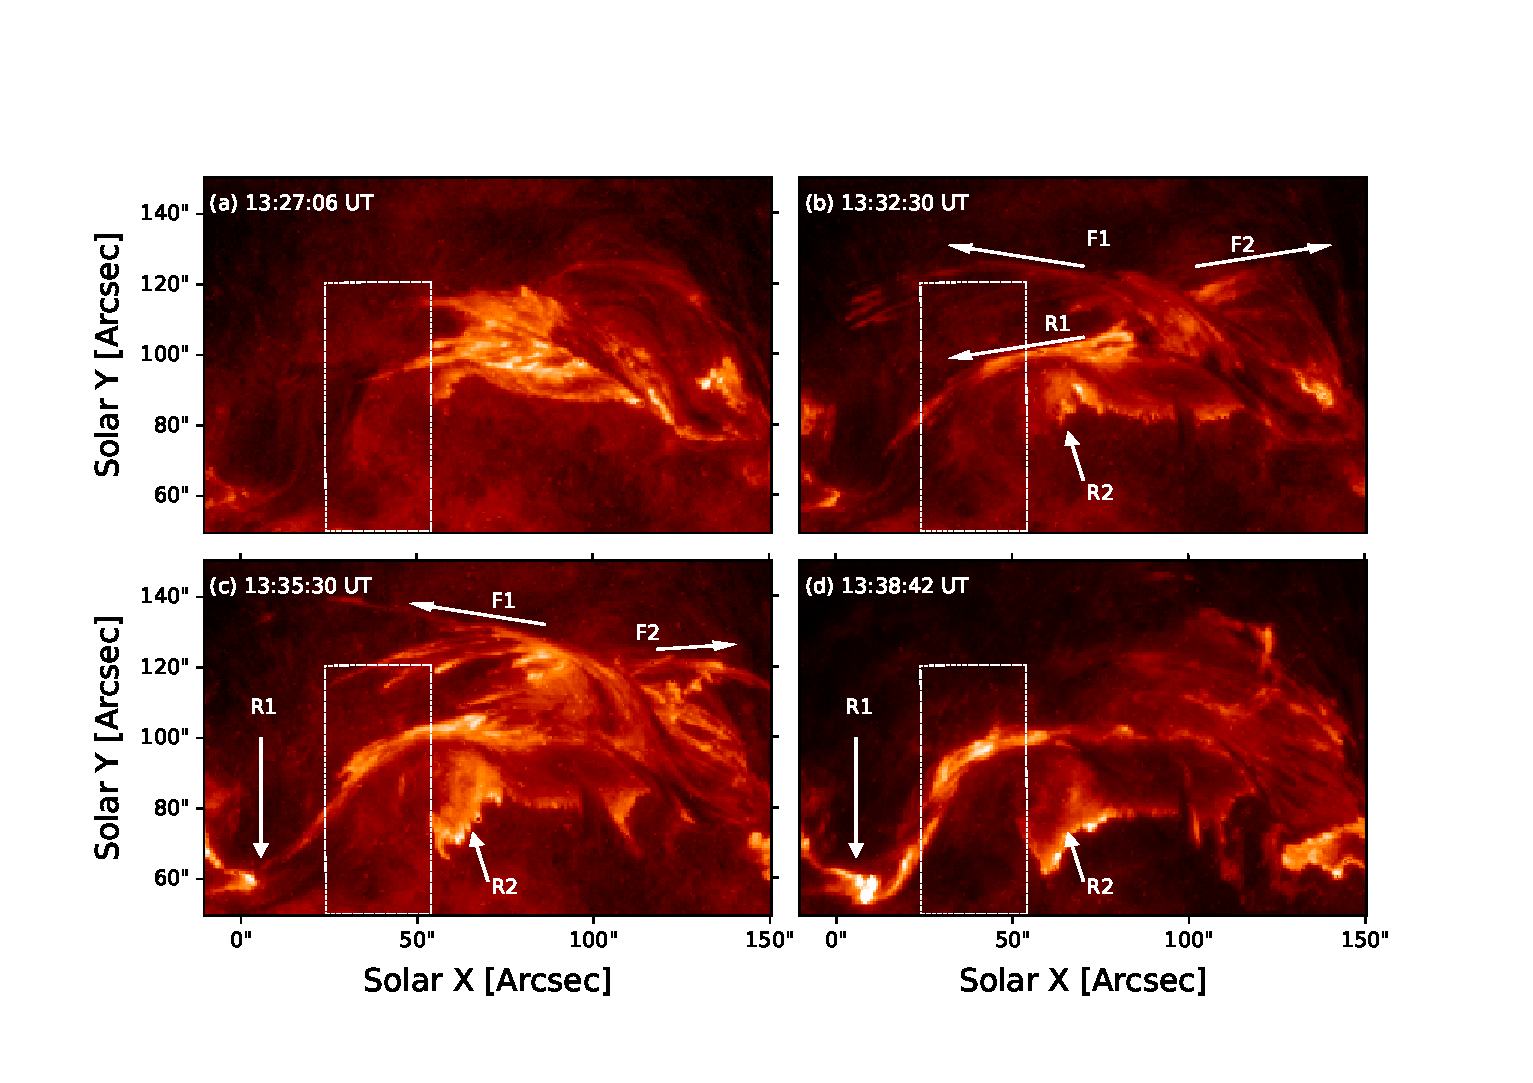
\includegraphics[width=\textwidth]{Figures/nov_flare_304_aa_evolv.eps}
    \end{center}
    \caption{Sequence of AIA 304~{\AA}~images for the Nov 4th, 2015 flare. The white dotted box shows the portion of the IRIS raster FOV which scanned the ribbons. In panels b (c) F1 and F2 are the filament material, which move away from each other as the flare progresses. R1 and R2 in b (c,d) show the primary ribbons which move through the IRIS raster FOV. An animation of this image sequence is available in \cite{roy24}.}
    \label{flare_m_ev}
\end{figure*}
%%%--------------

Fig.\ref{flare_m_aia} presents the same region as depicted in Fig.\ref{flare_m_ev} across the six coronal channels (i.e., 94, 131, 171, 193, 211, 335~{\AA}) of SDO/AIA, recorded at the peak (top two rows) and during the decline phase (bottom two rows) of the flare. Post-eruption arcades \citep[][]{TriBC_2004} are clearly observable in all the channels, displaying slightly varied morphologies. These arcades contain evaporated thermal plasma and exhibit loop top brightening, likely due to colliding evaporation flows \citep[see, e.g.,][]{sharma16, patsourakos04}.

%%%--------------
\begin{figure*}[ht!]
    \begin{center}
        \includegraphics[trim={4.5cm 5.5cm 6cm 4cm},clip,width=\textwidth]{Figures/nov_flare_aia_waves_2.pdf}
    \end{center}
    \caption{The Nov 4th, 2015 flare in the six Coronal channels of the SDO/AIA at the soft X-ray peak (panels (a)-(f)) and during the decline phase (panels (g)-(l)) of the flare.}
    \label{flare_m_aia}
\end{figure*}
%%%--------------

We begin by aligning the HMI observations with the IRIS observations using the 1600~{\AA} data recorded by AIA. Given that the observation involves an active region undergoing flaring, the magnetic field may also be rapidly changing \citep{wang02,dandan16,spirock02}. Therefore, we utilize a series of co-aligned full-disk maps from AIA and HMI to derive a rastered line-of-sight (LOS) map of magnetic flux density that precisely corresponds to the location and time of IRIS rasters. This procedure is outlined below.

Initially, we align the AIA 1600~{\AA} observation with the HMI observation closest in time to the IRIS SJI (Slit-Jaw Imager) and raster observations. Using the `aia\_prep' tool available in the \textit{sswidl} distribution, we process the level 1 images to perform image registration and align AIA and HMI observations. Subsequently, we calculate the shift between AIA 1600~{\AA} and the SJI 1400~{\AA}. Using these calculated offsets, we co-align the magnetograms with the IRIS SJI 1400~{\AA} observations, given that the AIA 1600~{\AA} observation was already aligned with the HMI observations. We typically observe an offset of approximately $\sim$ 1.5\arcsec~between HMI and IRIS. These co-aligned HMI maps are then utilized to derive the rastered magnetograms, which can be directly compared with IRIS raster observations.

%%%%-------------------------
\begin{figure}[ht!]
\centering  
\vspace{10cm}
\includegraphics[trim={7cm 5cm 6cm 15cm},width=0.7\textwidth]{Figures/m_flare_iris.pdf}
\caption{Obtained images in  \ion{Mg}{2} h (panel a) and k (panel b) and corresponding co-aligned and artificially rastered HMI LOS magnetic field map (panel c) for the M3.7 flare observed on November 4th, 2015. The magenta and lime green contours on panel c show the contours of  \ion{Mg}{2}~h (panel a) and k (panel b) intensity.} \label{fig:aligned_raster}
\end{figure}
%%%%-------------------------

For analyzing the properties of the  \ion{Mg}{2} lines, we fit a double Gaussian profile to both the k and h lines with a linear background symmetric about the line core. If excess emission is detected compared to the fitted background and line profile for wavelengths lower than 2792~{\AA} and in-between 2798~{\AA} to 2800~{\AA}, we infer the presence of  \ion{Mg}{2} triplets in emission. A single Gaussian profile is fitted to the excess emission. It's important to note that this approach may overlook the triplets unless the emission is sufficiently strong. However, this method serves our purpose since our primary objective is to characterize the  \ion{Mg}{2} k and h line profiles.

Additionally, we exclude any pixels showing saturation in either of the lines. The uncertainty of the observed intensities is measured in DN (Data Numbers) using the method outlined in \S2.1 of \cite{kerr15} and subsequently applied in the fitting procedure. The uncertainties of the fitted Gaussian profiles are incorporated while integrating the profile to obtain the uncertainty of the line intensities.

%%%%%%%%%%%
\begin{figure*}[ht!]
    \centering
    \includegraphics[trim={0cm 3cm 0.5cm 3cm},clip,width=\textwidth]{Figures/pix_fit.pdf}
    \caption{Fit of the  \ion{Mg}{2} window for the pixel marked in northern ribbon (southern ribbon) in Fig.~\ref{fig:aligned_raster} in top panel (bottom panel) from various times during the evolution of the flare. }
    \label{fig:pix_fit_ribbon}
\end{figure*}
%%%%%%%%%%%

%%%%-------------------------
\begin{figure}[ht!]
\centering  
\includegraphics[trim={1.5cm 4cm 0.5cm 4cm},clip,width=0.8\textwidth]{Figures/m_flare_iris_pt2.pdf}
\caption{The 1{--}8~{\AA} GOES light curve of the flare over-plotted with the time variation of  \ion{Mg}{2} k/h line intensity ratio for the northern (black) and southern (green) asterisks marked in panels a, b \& c.}
\label{fig:aligned_iris_ratio}
\end{figure}
%%%%-------------------------

In Figure~\ref{fig:aligned_raster}, we present intensity maps obtained in  \ion{Mg}{2} h \& k (panels a \& b) alongside the rastered line-of-sight (LOS) magnetic field map in panel (c). The dashed magenta and solid green contours on the magnetic field maps represent the intensity from panels a and b, respectively. To investigate the  \ion{Mg}{2} k to h intensity line ratios over time, we selected two pixels—one in the northern ribbon and another in the southern ribbon, as indicated by crosses. Fig.~\ref{fig:pix_fit_ribbon} displays the spectra overlaid with fits for the two pixels taken in the northern ribbon (top panel) and southern ribbon (bottom panel) obtained at different times.

We illustrate the  \ion{Mg}{2} k to h line intensity ratio derived from the two locations in the northern (black) and southern ribbons (green) in Fig.\ref{fig:aligned_iris_ratio}. Additionally, we overlay the GOES light curve of the flare obtained in 1.0{--}8.0{\AA} (red solid line). Our observations indicate that the intensity ratios exhibit a slightly increasing trend, albeit within the margin of errors, during the early phase of the flare. The ratio demonstrates a distinct peak around the midpoint of the impulsive phase, lasting for a very brief duration of approximately 150 seconds, before beginning to decrease. It's worth emphasizing that the pixel-by-pixel fitting of the  \ion{Mg}{2} h \& k line profiles provided a sufficient signature of the time evolution of the k/h line intensity ratio during the flare.

%%%%%%%--------%%%%%%%%%%%
\subsection{Investigating the dependence on the local magnetic field in the  \ion{Mg}{2} lines}
%%%%%%%---------%%%%%%%%%%

To explore the time evolution of the intensity ratio and its potential relationship with the photospheric magnetic field, we binned the spectra into various magnetic field bins from different flaring pixels. We selected the flaring pixels based on an intensity threshold relative to the peak intensity observed in IRIS rasters. A double Gaussian fit with a constant background was performed in a smaller wavelength window for both the  \ion{Mg}{2} h and k lines separately. This step was essentially carried out to mitigate the effects of the background and potential contributions from other spectral features.

Fig.~\ref{fig:fit_pix_fov} displays the  \ion{Mg}{2} k line profiles obtained at different times and averaged over different magnetic field bins. Each plot denotes the observation time and the magnetic field strength over which the spectra were averaged and fitted with a double Gaussian. Line intensities were computed by integrating the fitted Gaussian.

In Fig.~\ref{fig:optical_depth_m}, we present the k to h intensity ratios obtained in various bins of magnetic flux density at different times corresponding to different flare phases. The curve corresponding to 13:07:05 UT (red) represents the pre-flare phase, where the ratio is approximately 1.2. The ratio shows an increase during the impulsive phase, i.e., the curves corresponding to 13:23:44 UT (blue dotted) and 13:32:04 UT (green dashed). The ratio measured at 13:41:11 UT (magenta dashed), which is closest to the UV peak of the flare, exhibits the largest value across all magnetic field bins. Subsequently, during the decline phase, the ratio measured at 13:57:23 UT (black solid) falls below the values observed during the pre-flare phase. Additionally, it's noteworthy that there are no significant differences among the k to h ratios obtained in different bins of magnetic flux density at all times (including pre-flare, impulsive, peak, and decline phases) of the flare.

%%%%-----------------------
\begin{figure*}[ht!]
    \begin{center}
    \includegraphics[trim={0cm 3cm 0cm 3cm},clip,width=\textwidth]{Figures/binned_fit_fov.pdf}
    \end{center}
    \caption{Fitted line profiles for the binned spectra for various magnetic field strengths from various times.}
    \label{fig:fit_pix_fov}
\end{figure*}
%%%%----------------------- 

%%----------------------------------------------------------------------------
\begin{figure}[ht!]
    \centering
    \includegraphics[trim={8cm 1cm 2cm 0.2cm},clip,width=0.9\textwidth]{Figures/Flare-m-optical-depth-2.jpeg}
    \caption{ \ion{Mg}{2} k to h line intensity ratio for various magnetic flux density bins at various time steps during the evolution of the flare.}
    \label{fig:optical_depth_m}
\end{figure}
%%----------------------------------------------------------------------------

To explore further, we study the evolution of k to h intensity ratio as a function of time during the flare. In Fig.~\ref{fig:optical_dep_ev_m}, we plot the time evolution of the k to h line intensity ratio averaged within the bins of different magnetic flux densities as a function of time. For better visibility the 20.9{--}184.4 G and 348.9{--}513.3 G points are offset by 30s and -30s, respectively. We also plot the GOES 1{--}8~{\AA} light curve with the red solid line. These plots conspicuously reveal that the intensity ratios rise sharply during the impulsive phase, from $\sim$ 1.20 to $\sim$ 1.28 right before the soft X-ray flux peaks as seen from GOES, and decreases very rapidly thereafter, to lower than pre-flare values $\sim$ 1.12. The typical uncertainty value for the line intensity ratio is $\sim$ 0.02. We further note that the evolution of the  \ion{Mg}{2} k to h intensity ratio is remarkably similar across various strengths of magnetic flux densities.

%%%----------------------------------------------
\begin{figure*}[ht!]
    \centering
    \includegraphics[trim={3cm 3cm 2cm 4cm},clip,width=\textwidth]{Figures/Nov-11-2015-optical-dep-ev-5.pdf}
    \caption{Time evolution of the  \ion{Mg}{2} k to h line intensity ratio obtained from averaged spectrum over the corresponding magnetic flux bin as labeled for the Nov 4, 2015 flare. For better visibility, the 20.9{--}184.4 G and 348.9{--}513.3 G points are offset by 30s and -30s respectively. Over-plotted red solid line displays the 1{--}8~{\AA} GOES X-ray light curve.}
    \label{fig:optical_dep_ev_m}
\end{figure*}
%%%----------------------------------------------

%%%----------------------------------------------
\subsection{X1.6 Flare Observed on Oct 22, 2014}
%%%----------------------------------------------

An X~1.6 flare occurred on October 22, 2014, observed in AR 12192. The flare commenced at 14:02 UT and peaked at 14:28 UT as observed by GOES. Fig.\ref{flare2}(a) illustrates the GOES flux plot of the flare in the 0.5{--}4~{\AA} range (blue) and the 1.0{--}8.0~{\AA} range (red). Figs.\ref{flare2}(b) \& (c) display an AIA 1600{\AA} image and the line-of-sight (LOS) magnetic flux density map obtained from HMI, respectively. The overlaid boxes in panels (b) and (c) indicate the IRIS SJI (Slit-Jaw Imager) field of view (FOV). IRIS observed this flare with a large 8-step coarse raster covering a FOV of [14\arcsec,174\arcsec]. It's worth noting that the IRIS SJI FOV and the slit direction were rotated by approximately 45$^\circ$ relative to the center of the HMI observation.

%%--------------------------------------------------
\begin{figure}[ht!]
    \centering
\hspace*{-.5in}
\includegraphics[width=\textwidth,trim={7cm 5cm 7.7cm 6cm},clip]{Figures/Flare_X_oct22_2014_2.eps}
\caption{The X class flare observed on October 22, 2014. Panel a: GOES flux plot in 0.5{--}4~{\AA} (blue) and 1.0{--}8.0~{\AA} (red). Panel b: AIA 1600~{\AA} image taken at the peak of the flare. Arrows locate the primary and secondary ribbons. Panel c: LOS magnetic flux density map obtained from HMI at the peak of the flare. The over-plotted white (black) box in panel b (c) represents the IRIS SJI FOV, and white dot-dashed (dashed) box in panels b (c) represents the IRIS Raster FOV.}\label{flare2}
\end{figure}
%%--------------------------------------------------

The flare manifests two ribbons in AIA 1600{\AA}, as indicated by the arrows. The eastern ribbon extends around a negative field region and is entirely covered by the IRIS SJI FOV. Conversely, the western ribbon extends around a positive field region, with only a portion of it covered by the IRIS SJI FOV, as depicted in panel (b). In Fig.~\ref{fig:align_raster_flare2}, we present intensity maps obtained in  \ion{Mg}{2} h \& k (panels a \& b) alongside the rastered line-of-sight (LOS) magnetic field map (panel c). The black \& green dashed contours in the LOS magnetic field map (panel c) indicate the intensity contours of  \ion{Mg}{2} h \& k (panels a \& b).

%%--------------------------------------------------
\begin{figure}[ht!]
    \centering
%    \hspace{2in}
    \includegraphics[trim={6cm 3cm 6cm 3cm},clip,width=0.45\textwidth]{Figures/contour_paper_plot_oct28.pdf}
    \includegraphics[trim={3cm 2cm 2cm 3cm},clip,width=0.45\textwidth]{Figures/Oct-22-2014-optical-dep-ev-2.pdf}
    \caption{Obtained intensity maps in  \ion{Mg}{2}~k (panel a) and h (panel b) lines at the peak of the flare. The rastrered HMI LOS magnetic field density map is shown in panel c. The black and lime green contours on panel c show the contours of  \ion{Mg}{2}~k (panel a) and h (panel b) intensity.}
\label{fig:align_raster_flare2}
\end{figure}
%%--------------------------------------------------

Similar to the M-class flare studied in the previous section, we derive the  \ion{Mg}{2} k to h line intensity ratio for various bins of the magnetic flux density within the flaring region and study their time evolution. In Fig.\ref{fig:align_raster_flare2} right panel, we plot the intensity ratio in black and magenta colors for two different magnetic field bins. In the same panel, we also overlay the 1{--}8~{\AA} GOES light curve (red solid line). We note that, unlike the M-class flare, we do not observe any noticeable change in the intensity ratio during the flare. There are approximately two to three data points showing an enhancement in the ratio, but these occur well before the onset of the flare.

%%%----------------------------------------------
\subsection{C3.5 Flare Observed on Feb 03, 2015}
%%%----------------------------------------------

On February 3, 2015, AR 12277 generated a C-class flare that peaked at 22:55 UT. Fig.\ref{flare3} depicts the GOES flux plot of the flare in the 0.5{--}4{\AA} range (blue) and the 1.0{--}8.0~{\AA} range (red) in panel (a). Fig.\ref{flare3}(b) \& (c) displays an AIA 1600{\AA} image and the line-of-sight (LOS) magnetic flux density map obtained from HMI, respectively, recorded near the peak of the flare.

The overlaid white (black) box in panel (b) ((c)) indicates the IRIS SJI (Slit-Jaw Imager) field of view (FOV). The over-plotted white dot-dashed (magenta dashed) box in panel (b) ((c)) indicates the IRIS raster FOV. IRIS observed this flare with a large dense 16-step raster with a FOV of 5"$\times$119" and a step size of 0.35\arcsec. The flare exhibits a double ribbon structure, with the east ribbon elongating earlier and merging into the west ribbon. The IRIS raster scans through the west edge of the west ribbon through its eruption and merging with the east ribbon. Fig.~\ref{fig:align_raster_flare3} displays the intensity maps obtained in  \ion{Mg}{2} h \& k (panels a \& b). The rastered LOS magnetic field map is shown in panel (c). The black \& green dashed contours in the LOS magnetic field map (panel c) depict the intensity contours of  \ion{Mg}{2} h \& k (panels a \& b).

%%--------------------------------------------------
\begin{figure*}[ht!]
    \centering
\hspace*{-.6in}
\includegraphics[width=1.12\textwidth,trim={7cm 5cm 7.7cm 6cm},clip]{Figures/Flare_C_feb03_2015_2.eps}
%\includegraphics[width=.7\textwidth]{figures/Feb_03_2015/Feb-04-2015-optical-dep-ev-2.eps}
\caption{The C class flare observed on February 3rd, 2015. Panel a: GOES flux plot in 0.5{--}4~{\AA} (blue) and 1.0{--}8.0~{\AA} (red). Panel b: AIA 1600~{\AA} image of the flaring region. Panel c: LOS magnetic flux density map obtained from HMI near the peak of the flare. The over-plotted white (black) boxes in panel b (c) represents the IRIS SJI FOV. The over-plotted white dot-dashed (magenta dashed) box in panel b (c) show the IRIS raster FOV.}\label{flare3}
\end{figure*}
%%--------------------------------------------------

%%--------------------------------------------------
\begin{figure}[ht!]
    \centering
%\hspace*{-1.in}
\includegraphics[width=0.5\textwidth,trim={4cm 5cm 4cm 4cm},clip]{Figures/contour_paper_plot_feb-03-2015.pdf}
\caption{Obtained intensity maps in  \ion{Mg}{2}~k (panel a) and h (panel b) lines at the peak of the flare. The rastrered HMI LOS magnetic field density map is shown in panel c. The black and lime green contours on panel c show the contours of  \ion{Mg}{2}~k (panel a) and h (panel b) intensity.}
\label{fig:align_raster_flare3}
\end{figure}
%%--------------------------------------------------

%%--------------------------------------------------
\begin{figure}[ht!]
    \centering
    \includegraphics[trim={2cm 3cm 2cm 3cm},clip,width=0.8\textwidth]{Figures/Feb-04-2015-optical-dep-ev-2.pdf}
    \caption{Time evolution of the  \ion{Mg}{2} k to h line intensity ratio obtained from averaged spectrum over the corresponding magnetic flux bin as labeled for the Feb 3, 2015 flare. Over-plotted red solid line displays the 1{--}8~{\AA} GOES X-ray light curve.}
    \label{fig:optical_dep_ev_c}
\end{figure}
%%--------------------------------------------------

We present the GOES 1{--}8~{\AA}light curve (red solid line) alongside the time evolution of the  \ion{Mg}{2} k to h line intensity ratio averaged within the bins of two different magnetic flux densities as a function of time in Fig.\ref{fig:optical_dep_ev_c}. The  \ion{Mg}{2} k to h line intensity ratio exhibits a similar variation as observed in the M-class flare. It peaks during the impulsive phase (k/h$\sim$ 1.12) and decreases to preflare values (k/h$\sim$ 1.09) during the decay phase of the flare, coinciding with the peak of the GOES light curve. It's worth noting that the change in the  \ion{Mg}{2} k to h line intensity ratio is less pronounced for this flare compared to the M-class event. However, we also observe that the ratio shows a persistent increase from the onset of the flare.

%%--------------------------------------------------
\section{Outlook}
%%--------------------------------------------------

The  \ion{Mg}{2}~k to h line intensity ratios serve as a valuable diagnostic for assessing the opacity of the local plasma and can provide insights into changes in the local plasma environment within the solar chromosphere during flares. In this study, we investigated the temporal variation of  \ion{Mg}{2}k to h line intensity ratios during the evolution of three flares classified as X-class, M-class, and C-class. We also examined the variation of intensity ratios across different magnetic flux density bins, utilizing observations from IRIS and HMI. Co-alignment of IRIS and HMI observations was achieved using 1600{\AA} images recorded by AIA.

It's well-documented that  \ion{Mg}{2} profiles exhibit significant spatial variations within flaring regions \citep{dalda23,panos18}. As we binned the IRIS observations based on magnetic field strength, it's important to note that any spatial variation is averaged out and not addressed in our analysis.

Our findings reveal that  \ion{Mg}{2} k to h line intensity ratios undergo changes during flares. For M-class and C-class flares, the ratio starts increasing at the onset of the flare, peaks roughly halfway through the impulsive phase, and then steeply declines thereafter (see Figs.\ref{fig:optical_dep_ev_m} \& \ref{fig:optical_dep_ev_c}). Moreover, the ratios drop even below pre-flare levels during the later stages of the flare (peak and decline phase). However, this behavior is observed only in M and C-class flares, not in X-class flares.

Our observations did not reveal any correlation between line intensity ratios and magnetic flux density. The line intensity ratios for different magnetic field strengths illustrated in Figs.\ref{fig:optical_depth_m},\ref{fig:optical_dep_ev_m},~\ref{fig:optical_dep_ev_c} indicate a consistent behavior from weak to strong magnetic field strengths. This suggests that the magnetic field similarly affects both  \ion{Mg}{2}~k and h lines, and such effects cancel out when taking the ratios.

\cite{kerr15} studied  \ion{Mg}{2}~k to h line intensity ratios and their temporal variation for individual pixels in both quiet Sun regions and flare locations. While no change in ratios was observed for the quiet Sun region, variations were noted in flaring pixels, suggesting possible differences in heating conditions between non-flaring and flaring atmospheres. However, no correlated change in the ratio with respect to the flare light curve was observed.

Our results align with those of \cite{kerr15}, wherein they also observe the highest change in the ratio during the impulsive phase of the flare, decreasing before the flare reaches its maximum in GOES 1{--}8~{\AA} observations. Such variations in the ratio may indicate changes in the optical depth of the local medium. During the impulsive phase, decreased optical depth might be attributed to localized heating and chromospheric evaporation, while during the decay phase, increased optical depth could be due to condensation and downflows. However, this interpretation remains speculative, particularly as we did not observe such effects in X-class flares.

The results obtained for M-class and C-class flares can be explained by the aforementioned scenario, but the findings for X-class flares are more ambiguous. We couldn't establish a clear distinction in the general properties of these three flares. Notably, while the C-class flare is confined, both M and X flares are eruptive. Therefore, it's plausible that in X-class flares, energy deposition occurs more impulsively and on a shorter timescale than can be sampled. This high impulsiveness may lead to a greater degree of ionization of the medium compared to the other two flares, as supported by the large number of saturated pixels in the data that were discarded. A more definitive conclusion would necessitate analysis of additional such flares, including numerical and theoretical modeling.

The SUIT has four separate narrow band filters for the Mg window, namely NB2 (Blue wing of  \ion{Mg}{2} k), NB3 ( \ion{Mg}{2} k), NB4 ( \ion{Mg}{2} h) and NB5 (Red wing of  \ion{Mg}{2} h). As mentioned in chapter \ref{c:chap2} SUIT observes the full-disk Sun continuously in NB4 with $\sim$ 1 minute cadence and full-disk observations in all eleven science filters every 90 minutes. With the full disk observations in all science filters, we can investigate the opacity variations continuously across various solar features with a cadence of 90 minutes with the NB3 and NB4 ratio. In flare mode, the observing filter sequence is customizable. With high cadence observations in NB3 and NB4, we can investigate the effect of flare heating on the local plasma environment via its manifestation in opacity.
%
\chapter{Effects of Solar flares on the local plasma environment from Mg II observations}\label{c:chap5}
\chaptermark{Solar flares Mg II}
\begin{quote}
{ ~~~~~~~This thesis chapter originally appeared in the literature as} \\
{{\em The Evolution of the Ratio of \ion{Mg}{2} Intensities During Solar Flares, Roy, S., \& Tripathi, D. 2024, ApJ, 964, 106, doi:\href{https://iopscience.iop.org/article/10.3847/1538-4357/ad2a46}{10.3847/1538-4357/ad2a46}}.}
\end{quote}
%\begin{abstract}

 %   The  \ion{Mg}{2}~k \& h line intensity ratios can be used to probe the characteristics of the plasma in the solar atmosphere. In this study, using the observations recorded by the Interface Region Imaging Spectrometer (IRIS), we study the variation of the  \ion{Mg}{2}~k \& h intensity ratio for three flares belonging to X-class, M-class, and C-class, throughout their evolution. We also study the k-to-h intensity ratio as a function of magnetic flux density obtained from the line-of-sight magnetograms recorded by the Helioseismic and Magnetic Imager (HMI) on board the Solar Dynamics Observatory (SDO). Our results reveal that while the intensity ratios are independent of magnetic flux density, they show significant changes during the evolution of the C-class and M-class flares. The intensity ratios start to increase at the start of the flare and peak during the impulsive phase before the flare peak and decrease rapidly thereafter. The values of the ratios fall even below the pre-flare level during the peak and decline phases of the flare. These results are important in the light of heating and cooling of localized plasma and provide further constraint on the understanding of flare physics.
    
%\end{abstract}
\justifying

%%----------------------------------------------------
\section{Introduction} \label{sec:intro}
%%----------------------------------------------------

Solar flares are the most energetic events on the Sun, where an enormous amount of magnetic free energy is released due to the reconfiguration of the coronal magnetic field. The released energy can cause particle acceleration, heating and flows in the solar atmosphere and a transient enhancement in solar radiative output. Notably, a significant portion of the radiated energy during flares originates from the dense chromosphere \citep{fletcher10,milligan14}. Therefore, examining chromospheric lines during flares offers valuable diagnostic tools for understanding the physics of solar flares and their impact on the local plasma environment.

The chromosphere emits radiation across various ultraviolet (UV) and optical lines. While many optical lines, such as H$\alpha$ and \ion{Ca}{2}, are routinely observed from ground-based telescopes, observations of the  \ion{Mg}{2} resonance lines have been relatively infrequent in the past. However, since the launch of the Interface Region Imaging Spectrograph (IRIS) \citep{iris}, regular monitoring of these lines with excellent spatial and spectral resolution has become possible.

The  \ion{Mg}{2} k and h lines represent transitions to the ground state from finely split upper levels ($3p~^{2}P_{\nicefrac{3}{2}}${--}$3s~^{2}S_{\nicefrac{1}{2}}$ and $3p ^{2}P_{\nicefrac{1}{2}}${--}$3s^{2}S_{\nicefrac{1}{2}}$), resulting in optically thick lines at wavelengths 2796.34~{\AA} ( \ion{Mg}{2} k) and 2803.52{\AA} ( \ion{Mg}{2} h). It has been suggested that the intensity ratios of these lines can offer insights into the optical depth of the local environment \citep{kerr15}.

The integrated intensity of a line transitioning from an upper level $j$ to a lower level $i$ depends on the collision strength $\Omega_{ij}$ for that transition, given by~\citep{henri62,mariska92},

%%---------------------------------------------------------------
\begin{equation*}
\Omega_{ij}=\frac{8\pi}{\sqrt{3}}~\frac{I_{H}}{\Delta \epsilon_{ij}}g\omega_{i}~f_{ij}
\end{equation*}
%%---------------------------------------------------------------

\noindent Here, $I_{H}$ denotes the ionization energy of hydrogen, $\Delta \epsilon_{ij}$ represents the threshold energy for the transition, $g$ is the Gaunt factor, $\omega_{i}$ is the statistical weight of the level, and $f_{ij}$ stands for the oscillator strength. In optically thin conditions, the intensity ratio of the k to h line equals the ratio of collision strengths, as the escape probability of photons is unity. As the  \ion{Mg}{2} k and h lines share the same ionization state and originate from a transition to a shared lower level, and given that the statistical weight ($\omega_{i}$) is the same in both cases, the line intensity ratio is simply the ratio of oscillator strengths ($f_{ij}$). Consequently, this ratio is expected to be 2:1 in optically thin conditions and lower when the medium is optically thick \citep{kerr15,levens19}.

Moreover, the  \ion{Mg}{2} k and h lines can serve to estimate velocity in the middle and upper chromosphere, chromospheric velocity gradients, and temperature in the middle chromosphere \citep{leenarts13a,leenarts13b,pereira13}. Emission from the  \ion{Mg}{2} triplets can help identify heating in the lower chromosphere \citep{pereira15}. Various studies have demonstrated spatial variations in  \ion{Mg}{2} line profiles \citep{dalda23,panos18}. For instance, \cite{polito23} associated the leading edge of flare ribbons with enhanced broadening and strong central reversal, interpreting this difference in profile as indicative of distinct heating mechanisms at different locations within flare ribbons. Similarly, \cite{panos21,panos21_2} revealed differences in line profiles and energy input.

Using observations recorded by the OSO-8 LPSP instrument, \citep{lemaire84} investigated the evolution of intensity ratios of  \ion{Mg}{2} h \& k, \ion{Ca}{2} h \& k, and Ly$\alpha$ \&~$\beta$ lines. They observed that the intensity ratio of the \ion{Ca}{2}~k/h lines increased from 1 to 1.2 during the ascending phase of a flare and returned to 1 during later phases. This correlated temporal behavior across various elements was interpreted as an indication of downward energy propagation, suggesting a potential decrease in opacity due to localized heating at the formation height of the \ion{Ca}{2} line during the flare's rise phase.

Here, we investigate the evolution of intensity ratios of the  \ion{Mg}{2} h \& k lines during three flares: C-class, M-class, and X-class. Specifically, we focus on the dependence of line ratios on the underlying magnetic field strength, a relationship that, to our knowledge, has not been explored previously. The remainder of this chapter is organized as follows. Section \ref{sec:obs} presents the observations utilized in this study, followed by our data reduction and analysis methods, and the results in Section \ref{sec:dar}.

%%----------------------------------------------------
\section{Observations} \label{sec:obs}
%%----------------------------------------------------
%%-------------------------------------------------------
\begin{table*}[ht!]
\centering
\begin{tabular}{|c|c|c|c|c|c|}
\hline
Event & Flare & Flare & Raster & Raster Step & Raster \\
Date & Peak (UT) & Location (arcsec) & Details & (arcsec) & Cadence (s)\\
\hline
Nov 4, 2015  & 13:52 & [37",61"] & Coarse & 2" & 50\\
(M-class) & & & 16-step  & & \\
 & & & & & \\
Oct 22, 2014 & 14:28 & [-292",-302"] & Coarse & 2" & 131\\
(X-class) & & & 8-step  & & \\
 & & & & & \\
Feb 3, 2015 & 22:55 & [198",213"] & Dense & 0.35" & 33\\
(C-class) & & & 16-step  & & \\
\hline
\end{tabular}%}
%\end{center}
\caption{List of flares studied in this chapter.}
\label{tab:my_label}
\end{table*}
%%-------------------------------------------------------

For this study, we selected three flares of M, X, and C classes, as listed in Table~\ref{tab:my_label} by IRIS. IRIS is a NASA small explorer-class solar observation satellite that obtains UV spectra with high spatial (0.33{--}0.4\arcsec per pixel), temporal (1s), and spectral resolution ($\sim$26 and $\sim$53~m{\AA}). The primary lines regularly observed by IRIS include \ion{C}{2},  \ion{Mg}{2}, and \ion{Si}{4}. In the imaging channel, it typically observes in  \ion{Mg}{2} and \ion{Si}{4}. In our study, we utilized observations recorded in the  \ion{Mg}{2} h\& k lines.

As mentioned earlier, this study aims to analyze the evolution of intensity ratios concerning magnetic flux density during the flares of various classes. To achieve this, we incorporated line-of-sight (LOS) magnetic field measurements from the Helioseismic and Magnetic Imager \citep[HMI;][]{hmi} on the Solar Dynamics Observatory \citep[SDO;][]{sdo}. We utilized observations taken at 1600~{\AA} by the Atmospheric Imaging Assembly \citep[AIA;][]{aia}, also onboard SDO, to co-align the IRIS observations with those from AIA and subsequently HMI.

%%----------------------------------------------------
\section{Data analysis and results} \label{sec:dar}
%%----------------------------------------------------
\subsection{M3.7 Flare Observed on Nov 4, 2015}
%%%----------------------------------------------
%%--------------------------------------------------

NOAA AR 12443 generated a multi-ribbon GOES class M3.7 flare on November 4, 2015, which commenced around 13:31 UT and peaked at approximately 13:52 UT, as observed from the GOES Soft X-ray (SXR) 1{--}8~{\AA} flux (Fig.\ref{flare1}a). This event occurred at approximately [37\arcsec,61\arcsec] heliographic position and was extensively observed by IRIS, AIA, and HMI. Fig.\ref{flare1}a illustrates the GOES flux plot of the flare in the 0.5{--}4~{\AA} range (blue) and the 1.0{--}8.0~{\AA} range (red). Fig.\ref{flare1} b depicts AIA 1600{\AA} image of the flaring region, showing two ribbons indicated by arrows. In panel (c), we present the line-of-sight (LOS) magnetic flux density map obtained from HMI, recorded nearly simultaneously with the AIA image shown in panel (b). The white (black) box overlaid on Fig.\ref{flare1}(b) (c) represents the IRIS SJI (Slit-Jaw Imager) field of view (FOV). The white dot-dashed (magenta dashed) box in Fig.\ref{flare1}b (c) indicates the IRIS raster FOV. The FOV of the SJI (approximately [120\arcsec~$\times$119\arcsec]) covers the central part of the flaring region, with a spectral sampling of approximately 0.05~{\AA}/pixel. \cite{li17} investigated the dynamics of the ribbons for this flare, while \cite{karlick18} studied the associated radio bursts.

%%--------------------------------------------------
\begin{figure*}[ht!]
    \centering
\includegraphics[trim={7cm 5cm 7.7cm 6cm},clip,width=\textwidth]{Figures/Flare_M_Nov04_2015_2.eps}
\caption{The M3.7 flare observed on November 4th, 2015. Panel a: GOES flux plot in 0.5{--}4~{\AA} (blue) and 1.0{--}8.0~{\AA} (red). Panel b: AIA 1600~{\AA} image of the flaring region. Arrows locate the primary ribbons. Panel c: LOS magnetic flux density map obtained from HMI near the peak of the flare. The over-plotted white (black) boxes in panel b (c) represent the IRIS SJI FOV. The over-plotted white dot-dashed (magenta dashed) box in panel b (c) shows the IRIS raster FOV.}\label{flare1}
\end{figure*}
%%--------------------------------------------------

Figure~\ref{flare_m_ev} illustrates the evolution of the flare in AIA 304~{\AA}. The flare is connected with a pre-existing filament that undergoes an eruption, splitting into two structures denoted as F1 \& F2 in Fig.\ref{flare_m_ev}(b) \& (c). These two filament structures diverge from each other in opposite directions. The flare generates two primary flare ribbons, labeled as R1 \& R2 in Fig.\ref{flare_m_ev}(b), (c) \& (d). Starting around 13:32 UT, R1 travels southeastward, crossing the IRIS raster FOV, indicated by the white dotted box in Fig.\ref{flare_m_ev}(a), (b), (c) \& (d). The IRIS raster monitors the movement of the northern ribbon R1 and the eastern edge of R2. An animated version of Fig.\ref{flare_m_ev} is available in the online journal for further details.

%%%--------------
\begin{figure*}[ht!]
    \begin{center}
    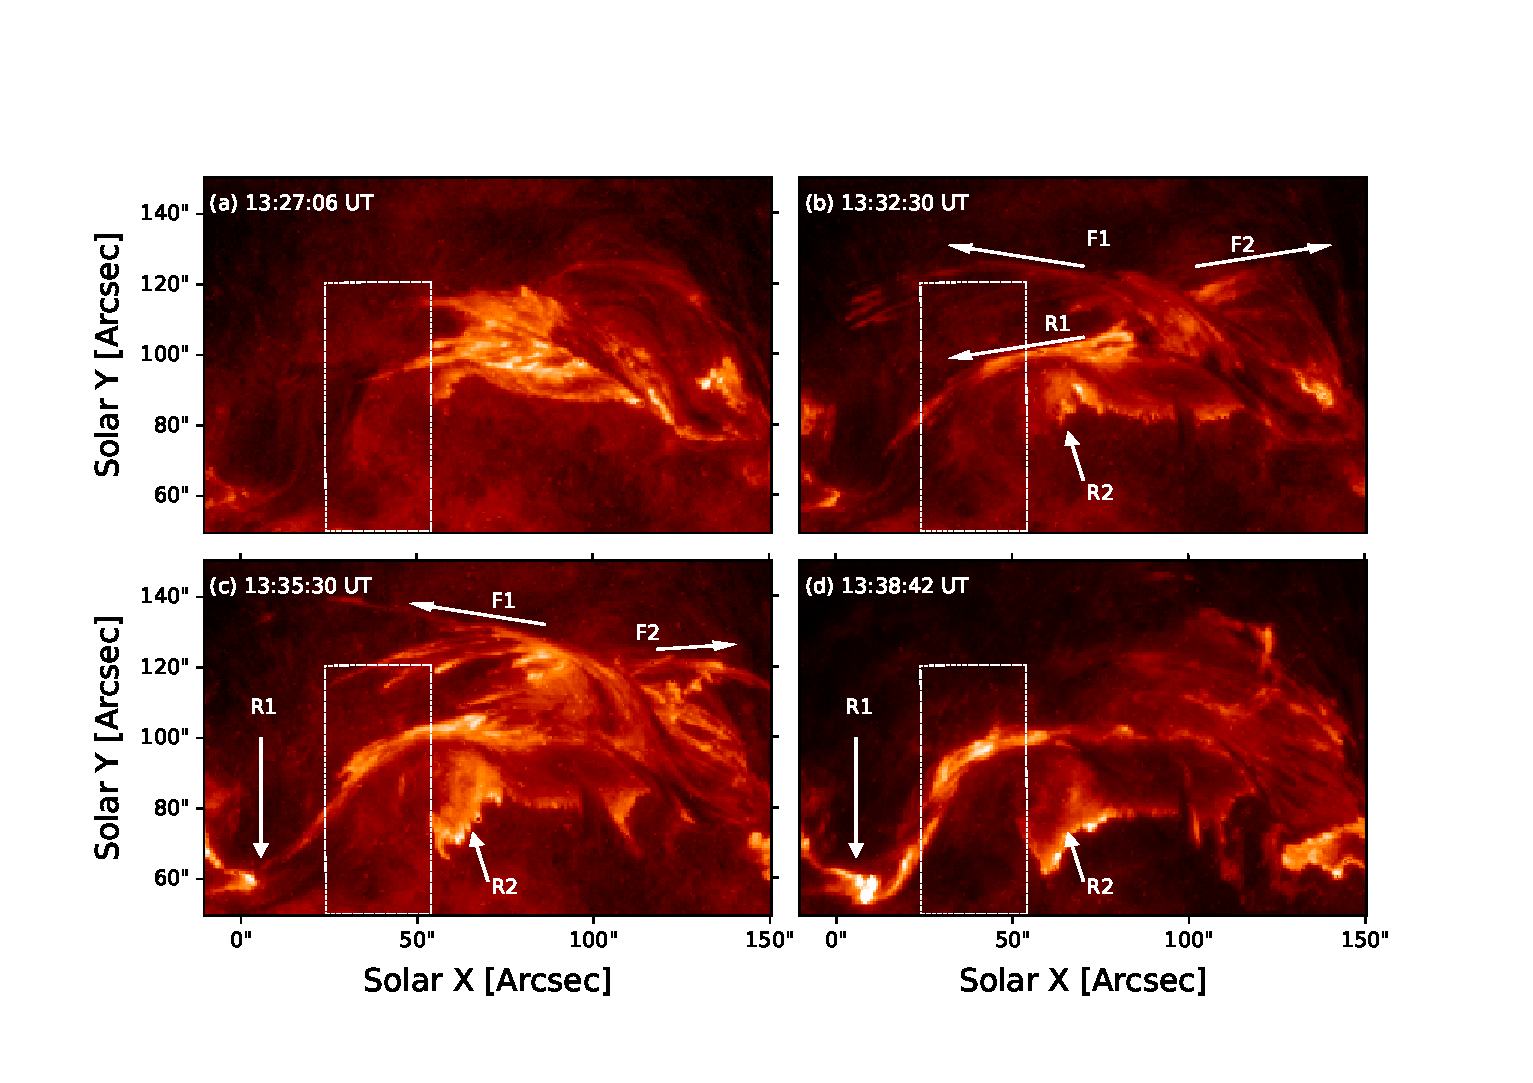
\includegraphics[width=\textwidth]{Figures/nov_flare_304_aa_evolv.eps}
    \end{center}
    \caption{Sequence of AIA 304~{\AA}~images for the Nov 4th, 2015 flare. The white dotted box shows the portion of the IRIS raster FOV which scanned the ribbons. In panels b (c) F1 and F2 are the filament material, which move away from each other as the flare progresses. R1 and R2 in b (c,d) show the primary ribbons which move through the IRIS raster FOV. An animation of this image sequence is available in \cite{roy24}.}
    \label{flare_m_ev}
\end{figure*}
%%%--------------

Fig.\ref{flare_m_aia} presents the same region as depicted in Fig.\ref{flare_m_ev} across the six coronal channels (i.e., 94, 131, 171, 193, 211, 335~{\AA}) of SDO/AIA, recorded at the peak (top two rows) and during the decline phase (bottom two rows) of the flare. Post-eruption arcades \citep[][]{TriBC_2004} are clearly observable in all the channels, displaying slightly varied morphologies. These arcades contain evaporated thermal plasma and exhibit loop top brightening, likely due to colliding evaporation flows \citep[see, e.g.,][]{sharma16, patsourakos04}.

%%%--------------
\begin{figure*}[ht!]
    \begin{center}
        \includegraphics[trim={4.5cm 5.5cm 6cm 4cm},clip,width=\textwidth]{Figures/nov_flare_aia_waves_2.pdf}
    \end{center}
    \caption{The Nov 4th, 2015 flare in the six Coronal channels of the SDO/AIA at the soft X-ray peak (panels (a)-(f)) and during the decline phase (panels (g)-(l)) of the flare.}
    \label{flare_m_aia}
\end{figure*}
%%%--------------

We begin by aligning the HMI observations with the IRIS observations using the 1600~{\AA} data recorded by AIA. Given that the observation involves an active region undergoing flaring, the magnetic field may also be rapidly changing \citep{wang02,dandan16,spirock02}. Therefore, we utilize a series of co-aligned full-disk maps from AIA and HMI to derive a rastered line-of-sight (LOS) map of magnetic flux density that precisely corresponds to the location and time of IRIS rasters. This procedure is outlined below.

Initially, we align the AIA 1600~{\AA} observation with the HMI observation closest in time to the IRIS SJI (Slit-Jaw Imager) and raster observations. Using the `aia\_prep' tool available in the \textit{sswidl} distribution, we process the level 1 images to perform image registration and align AIA and HMI observations. Subsequently, we calculate the shift between AIA 1600~{\AA} and the SJI 1400~{\AA}. Using these calculated offsets, we co-align the magnetograms with the IRIS SJI 1400~{\AA} observations, given that the AIA 1600~{\AA} observation was already aligned with the HMI observations. We typically observe an offset of approximately $\sim$ 1.5\arcsec~between HMI and IRIS. These co-aligned HMI maps are then utilized to derive the rastered magnetograms, which can be directly compared with IRIS raster observations.

%%%%-------------------------
\begin{figure}[ht!]
\centering  
\vspace{10cm}
\includegraphics[trim={7cm 5cm 6cm 15cm},width=0.7\textwidth]{Figures/m_flare_iris.pdf}
\caption{Obtained images in  \ion{Mg}{2} h (panel a) and k (panel b) and corresponding co-aligned and artificially rastered HMI LOS magnetic field map (panel c) for the M3.7 flare observed on November 4th, 2015. The magenta and lime green contours on panel c show the contours of  \ion{Mg}{2}~h (panel a) and k (panel b) intensity.} \label{fig:aligned_raster}
\end{figure}
%%%%-------------------------

For analyzing the properties of the  \ion{Mg}{2} lines, we fit a double Gaussian profile to both the k and h lines with a linear background symmetric about the line core. If excess emission is detected compared to the fitted background and line profile for wavelengths lower than 2792~{\AA} and in-between 2798~{\AA} to 2800~{\AA}, we infer the presence of  \ion{Mg}{2} triplets in emission. A single Gaussian profile is fitted to the excess emission. It's important to note that this approach may overlook the triplets unless the emission is sufficiently strong. However, this method serves our purpose since our primary objective is to characterize the  \ion{Mg}{2} k and h line profiles.

Additionally, we exclude any pixels showing saturation in either of the lines. The uncertainty of the observed intensities is measured in DN (Data Numbers) using the method outlined in \S2.1 of \cite{kerr15} and subsequently applied in the fitting procedure. The uncertainties of the fitted Gaussian profiles are incorporated while integrating the profile to obtain the uncertainty of the line intensities.

%%%%%%%%%%%
\begin{figure*}[ht!]
    \centering
    \includegraphics[trim={0cm 3cm 0.5cm 3cm},clip,width=\textwidth]{Figures/pix_fit.pdf}
    \caption{Fit of the  \ion{Mg}{2} window for the pixel marked in northern ribbon (southern ribbon) in Fig.~\ref{fig:aligned_raster} in top panel (bottom panel) from various times during the evolution of the flare. }
    \label{fig:pix_fit_ribbon}
\end{figure*}
%%%%%%%%%%%

%%%%-------------------------
\begin{figure}[ht!]
\centering  
\includegraphics[trim={1.5cm 4cm 0.5cm 4cm},clip,width=0.8\textwidth]{Figures/m_flare_iris_pt2.pdf}
\caption{The 1{--}8~{\AA} GOES light curve of the flare over-plotted with the time variation of  \ion{Mg}{2} k/h line intensity ratio for the northern (black) and southern (green) asterisks marked in panels a, b \& c.}
\label{fig:aligned_iris_ratio}
\end{figure}
%%%%-------------------------

In Figure~\ref{fig:aligned_raster}, we present intensity maps obtained in  \ion{Mg}{2} h \& k (panels a \& b) alongside the rastered line-of-sight (LOS) magnetic field map in panel (c). The dashed magenta and solid green contours on the magnetic field maps represent the intensity from panels a and b, respectively. To investigate the  \ion{Mg}{2} k to h intensity line ratios over time, we selected two pixels—one in the northern ribbon and another in the southern ribbon, as indicated by crosses. Fig.~\ref{fig:pix_fit_ribbon} displays the spectra overlaid with fits for the two pixels taken in the northern ribbon (top panel) and southern ribbon (bottom panel) obtained at different times.

We illustrate the  \ion{Mg}{2} k to h line intensity ratio derived from the two locations in the northern (black) and southern ribbons (green) in Fig.\ref{fig:aligned_iris_ratio}. Additionally, we overlay the GOES light curve of the flare obtained in 1.0{--}8.0{\AA} (red solid line). Our observations indicate that the intensity ratios exhibit a slightly increasing trend, albeit within the margin of errors, during the early phase of the flare. The ratio demonstrates a distinct peak around the midpoint of the impulsive phase, lasting for a very brief duration of approximately 150 seconds, before beginning to decrease. It's worth emphasizing that the pixel-by-pixel fitting of the  \ion{Mg}{2} h \& k line profiles provided a sufficient signature of the time evolution of the k/h line intensity ratio during the flare.

%%%%%%%--------%%%%%%%%%%%
\subsection{Investigating the dependence on the local magnetic field in the  \ion{Mg}{2} lines}
%%%%%%%---------%%%%%%%%%%

To explore the time evolution of the intensity ratio and its potential relationship with the photospheric magnetic field, we binned the spectra into various magnetic field bins from different flaring pixels. We selected the flaring pixels based on an intensity threshold relative to the peak intensity observed in IRIS rasters. A double Gaussian fit with a constant background was performed in a smaller wavelength window for both the  \ion{Mg}{2} h and k lines separately. This step was essentially carried out to mitigate the effects of the background and potential contributions from other spectral features.

Fig.~\ref{fig:fit_pix_fov} displays the  \ion{Mg}{2} k line profiles obtained at different times and averaged over different magnetic field bins. Each plot denotes the observation time and the magnetic field strength over which the spectra were averaged and fitted with a double Gaussian. Line intensities were computed by integrating the fitted Gaussian.

In Fig.~\ref{fig:optical_depth_m}, we present the k to h intensity ratios obtained in various bins of magnetic flux density at different times corresponding to different flare phases. The curve corresponding to 13:07:05 UT (red) represents the pre-flare phase, where the ratio is approximately 1.2. The ratio shows an increase during the impulsive phase, i.e., the curves corresponding to 13:23:44 UT (blue dotted) and 13:32:04 UT (green dashed). The ratio measured at 13:41:11 UT (magenta dashed), which is closest to the UV peak of the flare, exhibits the largest value across all magnetic field bins. Subsequently, during the decline phase, the ratio measured at 13:57:23 UT (black solid) falls below the values observed during the pre-flare phase. Additionally, it's noteworthy that there are no significant differences among the k to h ratios obtained in different bins of magnetic flux density at all times (including pre-flare, impulsive, peak, and decline phases) of the flare.

%%%%-----------------------
\begin{figure*}[ht!]
    \begin{center}
    \includegraphics[trim={0cm 3cm 0cm 3cm},clip,width=\textwidth]{Figures/binned_fit_fov.pdf}
    \end{center}
    \caption{Fitted line profiles for the binned spectra for various magnetic field strengths from various times.}
    \label{fig:fit_pix_fov}
\end{figure*}
%%%%----------------------- 

%%----------------------------------------------------------------------------
\begin{figure}[ht!]
    \centering
    \includegraphics[trim={8cm 1cm 2cm 0.2cm},clip,width=0.9\textwidth]{Figures/Flare-m-optical-depth-2.jpeg}
    \caption{ \ion{Mg}{2} k to h line intensity ratio for various magnetic flux density bins at various time steps during the evolution of the flare.}
    \label{fig:optical_depth_m}
\end{figure}
%%----------------------------------------------------------------------------

To explore further, we study the evolution of k to h intensity ratio as a function of time during the flare. In Fig.~\ref{fig:optical_dep_ev_m}, we plot the time evolution of the k to h line intensity ratio averaged within the bins of different magnetic flux densities as a function of time. For better visibility the 20.9{--}184.4 G and 348.9{--}513.3 G points are offset by 30s and -30s, respectively. We also plot the GOES 1{--}8~{\AA} light curve with the red solid line. These plots conspicuously reveal that the intensity ratios rise sharply during the impulsive phase, from $\sim$ 1.20 to $\sim$ 1.28 right before the soft X-ray flux peaks as seen from GOES, and decreases very rapidly thereafter, to lower than pre-flare values $\sim$ 1.12. The typical uncertainty value for the line intensity ratio is $\sim$ 0.02. We further note that the evolution of the  \ion{Mg}{2} k to h intensity ratio is remarkably similar across various strengths of magnetic flux densities.

%%%----------------------------------------------
\begin{figure*}[ht!]
    \centering
    \includegraphics[trim={3cm 3cm 2cm 4cm},clip,width=\textwidth]{Figures/Nov-11-2015-optical-dep-ev-5.pdf}
    \caption{Time evolution of the  \ion{Mg}{2} k to h line intensity ratio obtained from averaged spectrum over the corresponding magnetic flux bin as labeled for the Nov 4, 2015 flare. For better visibility, the 20.9{--}184.4 G and 348.9{--}513.3 G points are offset by 30s and -30s respectively. Over-plotted red solid line displays the 1{--}8~{\AA} GOES X-ray light curve.}
    \label{fig:optical_dep_ev_m}
\end{figure*}
%%%----------------------------------------------

%%%----------------------------------------------
\subsection{X1.6 Flare Observed on Oct 22, 2014}
%%%----------------------------------------------

An X~1.6 flare occurred on October 22, 2014, observed in AR 12192. The flare commenced at 14:02 UT and peaked at 14:28 UT as observed by GOES. Fig.\ref{flare2}(a) illustrates the GOES flux plot of the flare in the 0.5{--}4~{\AA} range (blue) and the 1.0{--}8.0~{\AA} range (red). Figs.\ref{flare2}(b) \& (c) display an AIA 1600{\AA} image and the line-of-sight (LOS) magnetic flux density map obtained from HMI, respectively. The overlaid boxes in panels (b) and (c) indicate the IRIS SJI (Slit-Jaw Imager) field of view (FOV). IRIS observed this flare with a large 8-step coarse raster covering a FOV of [14\arcsec,174\arcsec]. It's worth noting that the IRIS SJI FOV and the slit direction were rotated by approximately 45$^\circ$ relative to the center of the HMI observation.

%%--------------------------------------------------
\begin{figure}[ht!]
    \centering
\hspace*{-.5in}
\includegraphics[width=\textwidth,trim={7cm 5cm 7.7cm 6cm},clip]{Figures/Flare_X_oct22_2014_2.eps}
\caption{The X class flare observed on October 22, 2014. Panel a: GOES flux plot in 0.5{--}4~{\AA} (blue) and 1.0{--}8.0~{\AA} (red). Panel b: AIA 1600~{\AA} image taken at the peak of the flare. Arrows locate the primary and secondary ribbons. Panel c: LOS magnetic flux density map obtained from HMI at the peak of the flare. The over-plotted white (black) box in panel b (c) represents the IRIS SJI FOV, and white dot-dashed (dashed) box in panels b (c) represents the IRIS Raster FOV.}\label{flare2}
\end{figure}
%%--------------------------------------------------

The flare manifests two ribbons in AIA 1600{\AA}, as indicated by the arrows. The eastern ribbon extends around a negative field region and is entirely covered by the IRIS SJI FOV. Conversely, the western ribbon extends around a positive field region, with only a portion of it covered by the IRIS SJI FOV, as depicted in panel (b). In Fig.~\ref{fig:align_raster_flare2}, we present intensity maps obtained in  \ion{Mg}{2} h \& k (panels a \& b) alongside the rastered line-of-sight (LOS) magnetic field map (panel c). The black \& green dashed contours in the LOS magnetic field map (panel c) indicate the intensity contours of  \ion{Mg}{2} h \& k (panels a \& b).

%%--------------------------------------------------
\begin{figure}[ht!]
    \centering
%    \hspace{2in}
    \includegraphics[trim={6cm 3cm 6cm 3cm},clip,width=0.45\textwidth]{Figures/contour_paper_plot_oct28.pdf}
    \includegraphics[trim={3cm 2cm 2cm 3cm},clip,width=0.45\textwidth]{Figures/Oct-22-2014-optical-dep-ev-2.pdf}
    \caption{Obtained intensity maps in  \ion{Mg}{2}~k (panel a) and h (panel b) lines at the peak of the flare. The rastrered HMI LOS magnetic field density map is shown in panel c. The black and lime green contours on panel c show the contours of  \ion{Mg}{2}~k (panel a) and h (panel b) intensity.}
\label{fig:align_raster_flare2}
\end{figure}
%%--------------------------------------------------

Similar to the M-class flare studied in the previous section, we derive the  \ion{Mg}{2} k to h line intensity ratio for various bins of the magnetic flux density within the flaring region and study their time evolution. In Fig.\ref{fig:align_raster_flare2} right panel, we plot the intensity ratio in black and magenta colors for two different magnetic field bins. In the same panel, we also overlay the 1{--}8~{\AA} GOES light curve (red solid line). We note that, unlike the M-class flare, we do not observe any noticeable change in the intensity ratio during the flare. There are approximately two to three data points showing an enhancement in the ratio, but these occur well before the onset of the flare.

%%%----------------------------------------------
\subsection{C3.5 Flare Observed on Feb 03, 2015}
%%%----------------------------------------------

On February 3, 2015, AR 12277 generated a C-class flare that peaked at 22:55 UT. Fig.\ref{flare3} depicts the GOES flux plot of the flare in the 0.5{--}4{\AA} range (blue) and the 1.0{--}8.0~{\AA} range (red) in panel (a). Fig.\ref{flare3}(b) \& (c) displays an AIA 1600{\AA} image and the line-of-sight (LOS) magnetic flux density map obtained from HMI, respectively, recorded near the peak of the flare.

The overlaid white (black) box in panel (b) ((c)) indicates the IRIS SJI (Slit-Jaw Imager) field of view (FOV). The over-plotted white dot-dashed (magenta dashed) box in panel (b) ((c)) indicates the IRIS raster FOV. IRIS observed this flare with a large dense 16-step raster with a FOV of 5"$\times$119" and a step size of 0.35\arcsec. The flare exhibits a double ribbon structure, with the east ribbon elongating earlier and merging into the west ribbon. The IRIS raster scans through the west edge of the west ribbon through its eruption and merging with the east ribbon. Fig.~\ref{fig:align_raster_flare3} displays the intensity maps obtained in  \ion{Mg}{2} h \& k (panels a \& b). The rastered LOS magnetic field map is shown in panel (c). The black \& green dashed contours in the LOS magnetic field map (panel c) depict the intensity contours of  \ion{Mg}{2} h \& k (panels a \& b).

%%--------------------------------------------------
\begin{figure*}[ht!]
    \centering
\hspace*{-.6in}
\includegraphics[width=1.12\textwidth,trim={7cm 5cm 7.7cm 6cm},clip]{Figures/Flare_C_feb03_2015_2.eps}
%\includegraphics[width=.7\textwidth]{figures/Feb_03_2015/Feb-04-2015-optical-dep-ev-2.eps}
\caption{The C class flare observed on February 3rd, 2015. Panel a: GOES flux plot in 0.5{--}4~{\AA} (blue) and 1.0{--}8.0~{\AA} (red). Panel b: AIA 1600~{\AA} image of the flaring region. Panel c: LOS magnetic flux density map obtained from HMI near the peak of the flare. The over-plotted white (black) boxes in panel b (c) represents the IRIS SJI FOV. The over-plotted white dot-dashed (magenta dashed) box in panel b (c) show the IRIS raster FOV.}\label{flare3}
\end{figure*}
%%--------------------------------------------------

%%--------------------------------------------------
\begin{figure}[ht!]
    \centering
%\hspace*{-1.in}
\includegraphics[width=0.5\textwidth,trim={4cm 5cm 4cm 4cm},clip]{Figures/contour_paper_plot_feb-03-2015.pdf}
\caption{Obtained intensity maps in  \ion{Mg}{2}~k (panel a) and h (panel b) lines at the peak of the flare. The rastrered HMI LOS magnetic field density map is shown in panel c. The black and lime green contours on panel c show the contours of  \ion{Mg}{2}~k (panel a) and h (panel b) intensity.}
\label{fig:align_raster_flare3}
\end{figure}
%%--------------------------------------------------

%%--------------------------------------------------
\begin{figure}[ht!]
    \centering
    \includegraphics[trim={2cm 3cm 2cm 3cm},clip,width=0.8\textwidth]{Figures/Feb-04-2015-optical-dep-ev-2.pdf}
    \caption{Time evolution of the  \ion{Mg}{2} k to h line intensity ratio obtained from averaged spectrum over the corresponding magnetic flux bin as labeled for the Feb 3, 2015 flare. Over-plotted red solid line displays the 1{--}8~{\AA} GOES X-ray light curve.}
    \label{fig:optical_dep_ev_c}
\end{figure}
%%--------------------------------------------------

We present the GOES 1{--}8~{\AA}light curve (red solid line) alongside the time evolution of the  \ion{Mg}{2} k to h line intensity ratio averaged within the bins of two different magnetic flux densities as a function of time in Fig.\ref{fig:optical_dep_ev_c}. The  \ion{Mg}{2} k to h line intensity ratio exhibits a similar variation as observed in the M-class flare. It peaks during the impulsive phase (k/h$\sim$ 1.12) and decreases to preflare values (k/h$\sim$ 1.09) during the decay phase of the flare, coinciding with the peak of the GOES light curve. It's worth noting that the change in the  \ion{Mg}{2} k to h line intensity ratio is less pronounced for this flare compared to the M-class event. However, we also observe that the ratio shows a persistent increase from the onset of the flare.

%%--------------------------------------------------
\section{Outlook}
%%--------------------------------------------------

The  \ion{Mg}{2}~k to h line intensity ratios serve as a valuable diagnostic for assessing the opacity of the local plasma and can provide insights into changes in the local plasma environment within the solar chromosphere during flares. In this study, we investigated the temporal variation of  \ion{Mg}{2}k to h line intensity ratios during the evolution of three flares classified as X-class, M-class, and C-class. We also examined the variation of intensity ratios across different magnetic flux density bins, utilizing observations from IRIS and HMI. Co-alignment of IRIS and HMI observations was achieved using 1600{\AA} images recorded by AIA.

It's well-documented that  \ion{Mg}{2} profiles exhibit significant spatial variations within flaring regions \citep{dalda23,panos18}. As we binned the IRIS observations based on magnetic field strength, it's important to note that any spatial variation is averaged out and not addressed in our analysis.

Our findings reveal that  \ion{Mg}{2} k to h line intensity ratios undergo changes during flares. For M-class and C-class flares, the ratio starts increasing at the onset of the flare, peaks roughly halfway through the impulsive phase, and then steeply declines thereafter (see Figs.\ref{fig:optical_dep_ev_m} \& \ref{fig:optical_dep_ev_c}). Moreover, the ratios drop even below pre-flare levels during the later stages of the flare (peak and decline phase). However, this behavior is observed only in M and C-class flares, not in X-class flares.

Our observations did not reveal any correlation between line intensity ratios and magnetic flux density. The line intensity ratios for different magnetic field strengths illustrated in Figs.\ref{fig:optical_depth_m},\ref{fig:optical_dep_ev_m},~\ref{fig:optical_dep_ev_c} indicate a consistent behavior from weak to strong magnetic field strengths. This suggests that the magnetic field similarly affects both  \ion{Mg}{2}~k and h lines, and such effects cancel out when taking the ratios.

\cite{kerr15} studied  \ion{Mg}{2}~k to h line intensity ratios and their temporal variation for individual pixels in both quiet Sun regions and flare locations. While no change in ratios was observed for the quiet Sun region, variations were noted in flaring pixels, suggesting possible differences in heating conditions between non-flaring and flaring atmospheres. However, no correlated change in the ratio with respect to the flare light curve was observed.

Our results align with those of \cite{kerr15}, wherein they also observe the highest change in the ratio during the impulsive phase of the flare, decreasing before the flare reaches its maximum in GOES 1{--}8~{\AA} observations. Such variations in the ratio may indicate changes in the optical depth of the local medium. During the impulsive phase, decreased optical depth might be attributed to localized heating and chromospheric evaporation, while during the decay phase, increased optical depth could be due to condensation and downflows. However, this interpretation remains speculative, particularly as we did not observe such effects in X-class flares.

The results obtained for M-class and C-class flares can be explained by the aforementioned scenario, but the findings for X-class flares are more ambiguous. We couldn't establish a clear distinction in the general properties of these three flares. Notably, while the C-class flare is confined, both M and X flares are eruptive. Therefore, it's plausible that in X-class flares, energy deposition occurs more impulsively and on a shorter timescale than can be sampled. This high impulsiveness may lead to a greater degree of ionization of the medium compared to the other two flares, as supported by the large number of saturated pixels in the data that were discarded. A more definitive conclusion would necessitate analysis of additional such flares, including numerical and theoretical modeling.

The SUIT has four separate narrow band filters for the Mg window, namely NB2 (Blue wing of  \ion{Mg}{2} k), NB3 ( \ion{Mg}{2} k), NB4 ( \ion{Mg}{2} h) and NB5 (Red wing of  \ion{Mg}{2} h). As mentioned in chapter \ref{c:chap2} SUIT observes the full-disk Sun continuously in NB4 with $\sim$ 1 minute cadence and full-disk observations in all eleven science filters every 90 minutes. With the full disk observations in all science filters, we can investigate the opacity variations continuously across various solar features with a cadence of 90 minutes with the NB3 and NB4 ratio. In flare mode, the observing filter sequence is customizable. With high cadence observations in NB3 and NB4, we can investigate the effect of flare heating on the local plasma environment via its manifestation in opacity.
\clearpage
%
\chapter{Estimating thermal energy of two Solar Flares}\label{c:chap6}
\chaptermark{Solar flare energy}
\begin{quote}
{\em ~~~~~~~This thesis chapter originally appeared in the literature as} \\
{authors,
{\em journal reference info}}
\end{quote}
%\begin{abstract}

 %   The \ion{Mg}{2}~k \& h line intensity ratios can be used to probe the characteristics of the plasma in the solar atmosphere. In this study, using the observations recorded by the Interface Region Imaging Spectrometer (IRIS), we study the variation of the \ion{Mg}{2}~k \& h intensity ratio for three flares belonging to X-class, M-class, and C-class, throughout their evolution. We also study the k-to-h intensity ratio as a function of magnetic flux density obtained from the line-of-sight magnetograms recorded by the Helioseismic and Magnetic Imager (HMI) on board the Solar Dynamics Observatory (SDO). Our results reveal that while the intensity ratios are independent of magnetic flux density, they show significant changes during the evolution of the C-class and M-class flares. The intensity ratios start to increase at the start of the flare and peak during the impulsive phase before the flare peak and decrease rapidly thereafter. The values of the ratios fall even below the pre-flare level during the peak and decline phases of the flare. These results are important in the light of heating and cooling of localized plasma and provide further constraint on the understanding of flare physics.
    
%\end{abstract}

%%----------------------------------------------------
\section{Introduction} \label{sec:intro}
%%----------------------------------------------------

Solar flares are the most energetic events on the Sun, where an enormous amount of magnetic free energy is released due to the reconfiguration of the coronal magnetic field. The released energy can cause particle acceleration, heating and flows in the solar atmosphere and a transient enhancement in solar radiative output. It is observed that most of the energy radiated in flares originates from the dense chromosphere \citep{fletcher10,milligan14}. Hence, studying the chromospheric lines during flares provides us with diagnostics, which may be important for understanding the physics of solar flares and their effect on the local plasma environment.

The chromosphere emits in various UltraViolet(UV) and optical lines. While many optical lines, e.g., H$\alpha$, \ion{Ca}{2}, are routinely observed from ground-based telescopes, observations in the \ion{Mg}{2} resonance lines have been rare in the past. Since the launch of the Interface Region Imaging Spectrograph \citep[IRIS;][]{IRIS} we have been in the position to monitor these lines regularly with excellent spatial and spectral resolution.

The \ion{Mg}{2}~k and h lines are transitions to the ground state from a finely split pair of upper levels ($3p~^{2}P_{\nicefrac{3}{2}}${--}$3s~^{2}S_{\nicefrac{1}{2}}$ and $3p ^{2}P_{\nicefrac{1}{2}}${--}$3s~^{2}S_{\nicefrac{1}{2}}$). These transitions create the optically thick lines in the wavelengths 2796.34~{\AA} (\ion{Mg}{2}~k) and 2803.52~{\AA} (\ion{Mg}{2}~h). It is suggested that the intensity ratios of these lines can be used to probe the optical depth of the local environment \citep{kerr15}. 

The integrated intensity of a line transitioning from an upper-level j to a lower-level i, is dependent on the collision strength for that transition $\Omega_{ij}$, which is given by~\citep{henri62,mariska92},

%%---------------------------------------------------------------
\begin{equation*}
    \Omega_{ij}~=~\frac{8\pi}{\sqrt{3}}~\frac{I_{H}}{\Delta \epsilon_{ij}}~g~\omega_{i}~f_{ij}
\end{equation*}
%%---------------------------------------------------------------

\noindent Where $I_{H}$ is the ionization energy of Hydrogen, $\Delta \epsilon_{ij}$ is the threshold energy for the transition, g is the Gaunt factor, $\omega_{i}$ is the statistical weight of the level and $f_{ij}$ is the oscillator strength. In optically thin conditions, the intensity ratio of the k to h line is the ratio of the collision strengths, as the escape probability of photon is unity. The \ion{Mg}{2} k and h lines share the same ionization state and originate from a transition to a shared lowered level. As the statistical weight ($\omega_{i}$) is same in both cases, the line intensity ratio is simply the ratio of the oscillator strengths($f_{ij}$). This implies the ratio is 2:1 in optically thin conditions, and lower when the medium is optically thick \citep{kerr15,levens19}.

In addition, the \ion{Mg}{2} k and h lines can be used to estimate the velocity in the middle and upper chromosphere, the chromospheric velocity gradients, the temperature in the middle chromosphere \citep{leenarts13a,leenarts13b,pereira13}. The \ion{Mg}{2} triplets in emission can be used to identify heating in the lower chromosphere \citep{pereira15}. There have also been multiple studies that have shown a spatial variation of the \ion{Mg}{2} line profiles \citep{dalda23,panos18}. \cite{polito23} showed that the leading edge of the flare ribbon is associated with enhanced broadening and strong central reversal. They interpreted the difference in the profile as a difference in the heating mechanism at the leading edge and bright part of the flare ribbons. \cite{panos21,panos21_2} showed similar differences between the line profiles and energy input.

Using the observations recorded by the OSO-8 LPSP instrument, \citep{lemaire84} studied the evolution of the intensity ratio of \ion{Mg}{2}~h~\&~k, \ion{Ca}{2}~h~\&~k and Ly~$\alpha$~\&~$\beta$ lines. \cite{lemaire84} showed that the intensity ratio of the \ion{Ca}{2}~k/h lines increased from 1 to 1.2 during the ascending phase of a flare and returned to 1 during the later phases. The authors interpreted the correlated temporal behavior across various elements as an indication of downward energy propagation. We note that this may suggest a slight decrease in the opacity due to localized heating at the formation height of the \ion{Ca}{2} line during the rise phase of the flare.

%\sout{In spite of the excellent potential of these spectral lines in diagnosing the localized atmosphere, such} \sout{studies have not been taken up in detail due to the scarcity of spectral observations in these lines.}

Here, we study the evolution of the intensities ratios of the \ion{Mg}{2}~h~\&~k lines during the course of the evolution of three flares, \textit{viz.}, C-class, M-Class and X-class. We focus on the the dependence of line ratios on the underlying magnetic field strength, which to our knowledge has not been explored so far. The rest of the paper is structured as follows. \S\ref{sec:obs} discusses the observations used in this paper. We discuss how we reduce and analyze the data and the results in \S\ref{sec:dar}.
\clearpage
%
\chapter{First flares observed from {\suit}}\label{c:chap7}
\chaptermark{Solar flare energy}
\begin{quote}
{\em ~~~~~~~This thesis chapter originally appeared in the literature as} \\
{authors,
{\em journal reference info}}
\end{quote}
\justifying

%%----------------------------------------------------
\section{Introduction} \label{sec:intro}
%%----------------------------------------------------

The Solar Ultraviolet Imaging Telescope onboard {\it Aditya-L1} \citep[{\it Aditya-L1}/SUIT,][]{article,ghosh16,adityal1,suit_main} provides a targeted probe into the Chromosphere and Transition region. It provides continuous full-disk and Region of Interest (RoI) coverage of the Sun in eleven pass bands. The details of these bands are provided in chapter~\ref{c:chap3} Tab.~\ref{tab:science_filters}. The eight narrow bands provide coverage across the \ion{Mg}{2} k and h lines, \ion{Ca}{2} h line, the CN band, red and blue wing of the \ion{Mg}{2} window and parts of the NUV continuum. As alluded earlier, this provides unprecedented coverage of the Chromospheric and Transition region structure of solar flares.

The {\it Aditya-L1} was launched on September 2nd, 2023. The first light observations were made on December 5th, 2023 while the payload was still in cruise phase. For the majority of the cruise phase the payload only operated in the 2k synoptic mode, i.e. it only captured continuous (2k $\times$ 2k) observations in NB4 (\ion{Mg}{2} h line) with one minute cadence. The L1 insertion was carried out on January 6th, 2024. Following that the payload also started taking (4k $\times$ 4k) observations in all eleven science filters. Various components of the flare detection algorithm were progressively turned on. In this chapter we discuss some of the initial flare observations made by SUIT. The details of this flares are given in Tab.~\ref{f_list}. {\suit} observed an X5 flare on the east limb on 31st Dec, 2023 during its cruise phase. We primarily use observations from AIA with {\suit} observations to comment on the thermal structure and kinematics of the event.  We only have observations in the NB4 (\ion{Mg}{2} h line) channel for this flare as the observation is from during the cruise phase. The first flare triggered by the flare detection algorithm was a X6.3 flare from north-west corner of the disk on February 22nd, 2024, which was also observed by several other instruments {\it e.g.} {\it SDO}/AIA, {\it IRIS}, {\it SO}/STIX. The final flare discussed in this chapter is an X2.9 flare which occurred on 27th May, 2024 on the south east limb of the Sun. Subsequent portions of this chapter will be divided into three parts, where we discuss the observations of these three flares separately.

%----------------------------------------------------
\begin{table}[ht!]
\centering
\caption{Details of the flares studied in this chapter.}
\label{f_list}
\resizebox{0.6\linewidth}{!}{%
\begin{tabular}{lcr}
\hline
\hline
   Event Date  & Peak Time (UT) & Flare Location \\
\hline
2023 Dec 31 (X5) & 21:55 & [-968{\arcsec}, 88{\arcsec}] \\
2024 Feb 22 (X6.3) & 22:34 & [-400{\arcsec}, 350{\arcsec}]\\
2024 May 27 (X2.9) & 07:08 & [-920{\arcsec}, -250{\arcsec}] \\
\hline
\end{tabular}
}
\end{table}
%----------------------------------------------------

%%----------------------------------------------------
\section{X6.3 flare observed on Feb 22nd, 2024} \label{sec:feb_22nd}
%%----------------------------------------------------

NOAA AR 13590 was visible on the north-east of the Solar disk on February 22, 2024. The AR was around a large sunspot in a cluster of sunspots, accompanied by a complex magnetic field structure. The active region flared multiple times during the same day, including an X1.7 flare that peaked around $\sim$ 06:32 UT, an M4.8 flare that peaked around $\sim$ 20:46 UT and an X6.3 flare that peaked $\sim$ 22:34 UT . \suit~is equipped with an onboard flare detection algorithm. Once the flare detection algorithm flags a flare and localizes the position of the flare on the detector, the program sequence prioritizes reading a fixed smaller Region of Interest (RoI) around the location for fast, higher cadence observation (for further details, please refer to \cite{flare_det}). The X6.3 flare was one of the first flares to be localized by the on-board flare detection algorithm. \suit~did not observe the X1.7 flare because, during that time, the payload was off-pointed to verify the stellar calibration program sequences. The flares were also observed by {\it SDO}/AIA, {\it SO}/STIX. {\it IRIS} observed the eastern edge of the X6.3 flare ribbons in a small [66\arcsec,62\arcsec] field of view (FoV) with a 4 step raster and 15 s raster cadence.

We show the light curve arising from the whole RoI observation in comparison to {\it GOES} flux in Fig.~\ref{fig:flare_full}. In Fig.~\ref{fig:flare_full}.b, we plot the AIA 1600 {\AA} (dashed blue line) and AIA 1700 {\AA} (black dot-dashed line), in comparison to the {\it GOES} 1 {--} 8 {\AA} light curve (Solid red line) for both the flares. In Fig.~\ref{fig:flare_full}.b, we show the GOES 1 {--} 8 {\AA} light curve in comparison to the NB3 (\ion{Mg}{2} k 279.6 nm, black dotted), NB4 (\ion{Mg}{2} h 280.3 nm, green dot-dashed) and NB8 (\ion{Ca}{2} h 396.85 nm, magenta dashed) light curves. NB4 light curve is offset from NB3 by -0.1 for better visibility. The NB8 light curve exhibits lower contrast and does not show a sharp peak compared to NB3 and NB4. The other interesting trend is exhibited by the continuum channels NB5, NB6 and NB7 in Fig.~\ref{fig:flare_full}.c, as a conspicuous rise in the continuum intensity is seen after both flares. In Fig.~\ref{fig:flare_full}.d we plot the {\it GOES} 1 {--} 8 {\AA} light curve in comparison to the STIX hard (25 {--} 50 keV, black dashed) and soft (5 {--} 10 keV, green dotted) X-ray light curve. The hard X-ray observation from STIX peaks at a time similar to that of NB3, NB4, and NB8.

%%%%%%%%%
\begin{figure}[ht!]
    \centering
    \includegraphics[width=0.8\textwidth,trim={2.3cm 2.5cm 1cm 4.5cm},clip]{lc_full_suit_contour.pdf}
    \caption{Light curves from the whole RoI FoV of \suit~observations compared with AIA, {\it GOES} and STIX observation for the two flares.}
    \label{fig:flare_full}
\end{figure}
%%%%%%%%%

The X6.3 flare provides a good example of the response of the local plasma environment to the flare in the Near Ultraviolet (NUV) regime in 200 {--} 400 nm. The flare peaked around $\sim$ 22:34 UT in the {\it GOES} observation. Images from six narrow band (NB) channels of \suit~ are shown in Fig.~\ref{fig:flare_nb3_peak} top panel at around $\sim$ 22:28-22:29 UT. This is at the peak of the NB3 (\ion{Mg}{2} k 279.6 nm) channel, as observed by \suit. The 60\% peak intensity contour of the NB3 intensity is marked with the black line in all figures of Fig.~\ref{fig:flare_nb3_peak} top panel. From the figure, we also see a similar structure in the NB4 (\ion{Mg}{2} h 280.3 nm) and NB8 (\ion{Ca}{2} h 396.9 nm). No similar structure is observed in the other continuum channels of Fig.~\ref{fig:flare_nb3_peak} top panel.

In Fig.~\ref{fig:flare_nb3_peak} bottom panel, we show the flare observations by \suit~ at their respective peaks. Again, we see very similar structures in NB3, NB4, and NB8. NB3 and NB4 peak at almost the same time $\sim$ 22:29 UT. Although NB8 shows a similar structure, the peak intensity of NB8 is observed slightly later around $\sim$ 22:29:41 UT. The peak intensities of the other continuum NB channels are observed progressively later. The NB5 (Red wing of the Mg window) peaks around $\sim$ 22:32:41 UT. Faint signatures of flare brightening are observed in NB5, marked with red arrows in Fig.~\ref{fig:flare_nb3_peak} bottom panel. No such signatures are observed as clearly in NB6 and NB7. Both of these channels peak around $\sim$ 22:28 UT.

%%%%%%%%%
\begin{figure}[ht!]
    \centering
    \includegraphics[trim={0cm 0.65cm 0cm 0cm},clip,width=0.5\textwidth]{suit_roi_nb3_peak.pdf} \\
    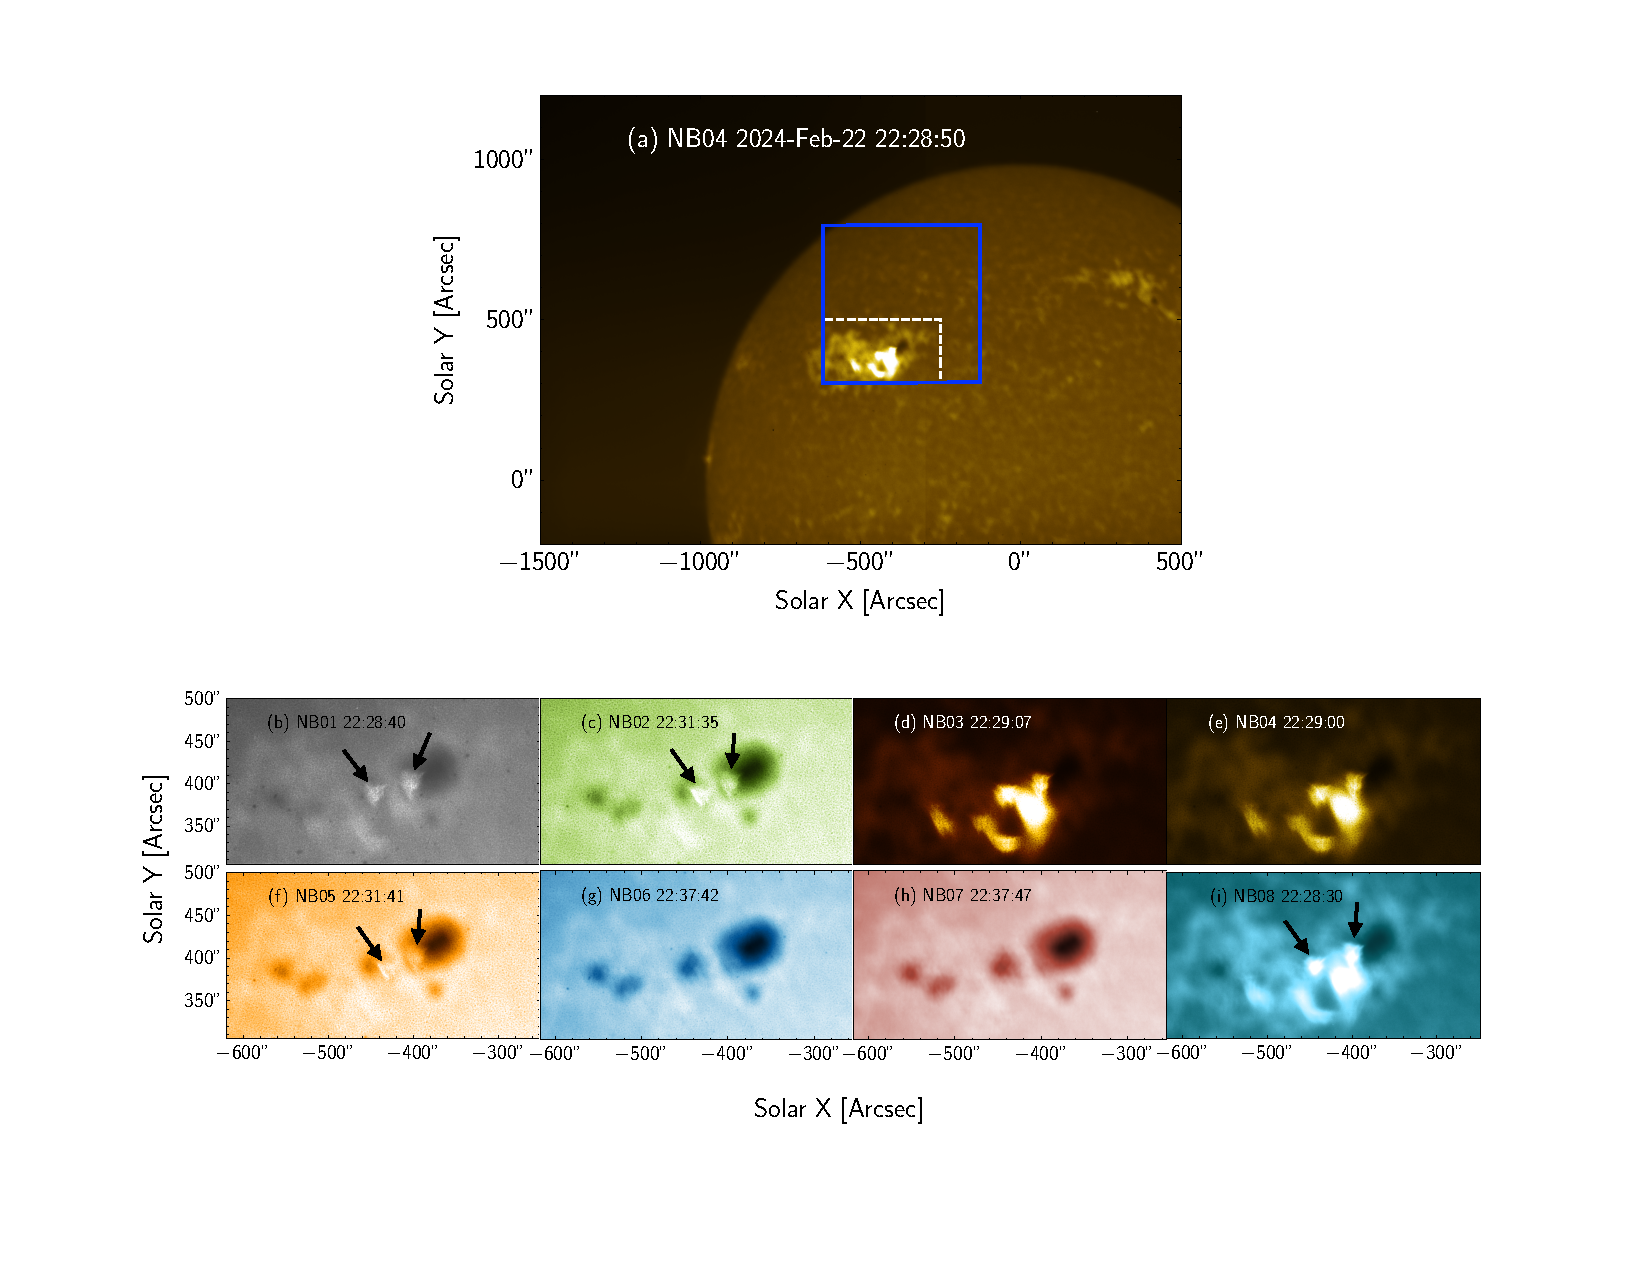
\includegraphics[width=0.5\textwidth]{suit_roi_all_peak.pdf}
    \caption{\suit~observations of the flare from various NB filters. Top panel: during NB3 peak. Bottom panel: During the peak of individual bands.}
    \label{fig:flare_nb3_peak}
\end{figure}
%%%%%%%%%

In Fig.~\ref{fig:flare_lc_suit}, we plot the light curve of the event to compare the observations across various bands. The AIA and \suit~ light curves in Fig.~\ref{fig:flare_lc_suit} are calculated by adding the counts within the region of 60\% peak intensity contour of NB3 (shown in Fig.~\ref{fig:flare_nb3_peak} top panel), after co-aligning and registering the AIA and \suit~observations and normalizing them to the peak intensity. In Fig.~\ref{fig:flare_lc_suit}.a, we show the GOES 1 {--} 8 {\AA} light curve in comparison to AIA 1600 {\AA} and AIA 1700 {\AA}. The AIA 1600 and 1700 {\AA} light curve peaks around $\sim$ 5 minutes earlier than the {\it GOES} peak. 

In Fig.~\ref{fig:flare_lc_suit}.b, we show the GOES 1 {--} 8 {\AA} light curve in comparison to the NB3, NB4 and NB8 light curves. All the NB light curves behave remarkably similarly. The vertical dotted black line across all the panels in Fig.~\ref{fig:flare_lc_suit} denotes the peak intensity in NB3. NB3, NB4, and NB8 peaks around $\sim$ 22:29 UT, which is very similar to AIA 1600 {\AA} and 1700 {\AA}. We also plot the {\it GONG}-H$\alpha$ light curve from the \suit~contour region. The {\it GONG} light curve also peaks at around $\sim$ 22:29 UT. Both NB8 and {\it GONG}-H$\alpha$ shows less contrast variation in the light curve than NB3 and NB4.

We show the GOES 1 {--} 8 {\AA} light curve in comparison to the NB5 (Red wing of the Mg lines, blue dashed), NB6 and NB7 continuum channels in Fig.~\ref{fig:flare_lc_suit}.c. NB5 shows signs of flare response, although much weaker than NB3, NB4 and NB8. NB5 peaks around $\sim$ 22:31 UT, about $\sim$ 3 minutes later than NB3. Similar traits were observed from the images also, as pointed out in Fig.~\ref{fig:flare_nb3_peak} bottom panel and the accompanying discussions. More interestingly, NB6 and NB7 do not show the hallmark sign of a flare light curve, i.e. gradual increase and decrease in the intensity. These bands exhibit a slow but steady rise in intensity after the flare. Finally, in Fig.~\ref{fig:flare_lc_suit}.d, we show the {\it GOES} 1 {--} 8 {\AA} light curve in comparison to the STIX hard and soft X-ray light curve. The hard X-ray peaks around a similar time around $\sim$ 22:29 UT, similar to NB3, NB4 and AIA 1600 and 1700 {\AA}.

%%%%%%%%%
\begin{figure}[ht!]
    \centering
    \includegraphics[width=0.8\textwidth,trim={2.3cm 2.5cm 0cm 4.5cm},clip]{lc_suit_contour.pdf}
    \caption{Light curves from the pixels within intensity contour picked from \suit~and co-aligned AIA observations. The NB4 light curve in the second panel is offset by -0.1 from NB3 for better visibility. The vertical dotted dark line marks the flare's peak in NB3 observation.}
    \label{fig:flare_lc_suit}
\end{figure}
%%%%%%%%%

%%%%%%% ############# %%%%%%%
\subsection{XSM-spectra}\label{sec:xsm}
%%%%%%% ############# %%%%%%%

The Solar X-ray monitor on {\it Chandrayan-2}\citep[{\it Chandrayan-2}/XSM,][]{xsm} provides sun as a star soft X-ray spectra in 1{--}15 keV with 1s cadence and significantly better spectral resolution (180 eV at 5.9 keV) compared to STIX (1 keV ar 5.9 keV). The high spectral and temporal resolution allows us to measure the change in elemental abundances over the duration of the flares. XSM observed both flares with coverage in both impulsive and decay phase. The existing studies with XSM has successfully studies the thermal and elemental abundance evolution of various flares \citep{mondal21,kkepa23,nama23}.

Both the M and X-class flares were observed by XSM. The XSM 1{--}8 {\AA} light curves are plotted in Fig.~\ref{fig:xsm-obs} top panel. The red shaded region marks the time window where the Be filter was inserted to prevent saturation. There are periodic gaps in the data due to periodic lunar occultation. We show the spectra obtained by XSM in Fig.~\ref{fig:xsm-obs} bottom panel, during various phases of the flare. The violet spectra at 22:33 UT is near the flare peak, and shows a sharp decrease below 3 keV due to the insertion of the Be filter to avoid saturation. Various Mg, Al, S and Si lines are visible in the pre-flare spectra. In stark contrast during impulsive and peak of the flare we see strong signatures of Ca, Ar and Fe. Due to the uncertainty of the spectra during the Be window observation in $<~3~\mathrm{keV}$ regime, we fit the spectra beyond 3 keV throughput this analysis. We fit the spectra with the XSPEC model {\it chisoth}, which uses a wide range of pre-calculated spectra to fit the observed spectra (For more details please refer to the appendix of \cite{mondal21}).

%%%%%%%%
\begin{figure}[ht!]
\centering
    \includegraphics[trim={0.5cm 3.3cm 0.8cm 4cm}, clip, width=0.76\textwidth]{xsm_lc.pdf} \\
    \includegraphics[trim={1.8cm 2.5cm 3cm 3cm},clip,width=0.75\textwidth]{xsm_spec.pdf}
    \caption{Top panel: XSM observation of the two flares. The red shaded region marks the window when the Be filter was inserted. Bottom panel: X-ray spectra during various phases of the flare. The violet spectra is during the soft X-ray peak of the flare and shows a sharp decrease in the intensity below 3 keV. This is due to the insertion of Be filter to avoid saturation.}
    \label{fig:xsm-obs}
\end{figure}
%%%%%%%%

%%%%%%% ############# %%%%%%%
\subsubsection{Fitting XSM spectra}\label{sec:xsm-fit}
%%%%%%% ############# %%%%%%%

The observed soft X-ray spectra from the flaring plasma can be modelled by an isothermal plasma characterized by various parameters {\it e.g.} temperature, emission measure and abundance of various elements. As alluded earlier, we use the `{\it chisoth}' model \citep{mondal21} to fit the observed spectra from XSM. The `{\it chisoth}' model uses CHIANTI atomic database \cite{chianti} to calculate spectra for individual elements over a large temperature grid and stores as tables. The model includes elements from H (Z=1) to Zn (Z=30). The spectra of individual elements are calculated over a wide temperature range (0.3 {--} 50 MK). These modelled spectra of various elemental abundance over a wide temperature range are loaded in XSPEC and added with varying weights to fit the observed spectra. The Total model spectrum is given by  $$I_{mod}(T)~=~EM\sum_{X}I_{X}(T)N_{X}$$`EM' is the volume emission measure, $N_{X}$ is the abundance of element X relative to H and $I_{X}(T)$ is the modelled spectrum of element X at temperature T. The fit is done in a recursive process by minimizing the chi-squared between the observed and modelled spectra.

We initially used an isothermal model to fit the spectra. One of the key observations we make is a presence of systematic residual around the Fe complex around $\sim$ 6.5 keV. This is illustrated in the top panel of Fig.~\ref{fig:xsm_fit} top panel, where there is an excess visible in the blue side of the Fe line complex at $\sim$ 6.7 keV. \cite{mithun22} could not explain this systematic excess with multithermal DEM distributions. One of the possible explanation of this excess flux is Fe fluorescence emission. There have been observations of Fe line fluorescence at 6.4 keV (Fe K$\alpha$) and 7.06 keV (Fe K$\beta$) \citep{neupert67,doscheck71,bai79,tanaka84,parmar84,phillips12} using high-resolution X-ray spectra from Bent Crystal Spectrometer on-board Solar Maximum Mission \citep[Bent/{\it SMM},][]{bent,smm} and Yokoh \citep{yokoh} mission. Previous studies have suggested that this emission arises from the excitation of low ionization state Fe in the Photosphere either via the X-ray from the flaring plasma \citep{bai79} or directly from the non-thermal electron beam \citep{phillips73}. The Fe K$\alpha$ fluorescence is usually dependent on the position on the solar disk \citep{parmar84}. The emergent Fe K$\alpha$ emission suffers significant absorption and scattering along the line of sight, which increases with increasing heliocentric angle, resulting in a decrease in the observed intensity. For our event, the flaring region is near the disk center making the Fe K$\alpha$ fluorescence a valid candidate for explaining the excess. We added a Gaussian component to the `{\it chisoth}' model to get better fit (see Fig.~\ref{fig:flare_obs} bottom panel).

We add a Gaussian line component to our fit at 6.4 keV to explore the possibility of the excess flux arising from Fe K$\alpha$ fluorescence. We find that this fits the observed spectra better than previous instances, as demonstrated in Fig.~\ref{fig:xsm_fit} bottom panel. The K$\alpha$ emission would arise from the X-ray emission from the flaring regions having energies $>$ 7.12 keV, the K edge of Fe, exciting the Fe atoms in the Photosphere. We show the intensity of the fitted Fe 6.4 keV component excess (blue solid line), in comparison to the fitted flux in 7.12 {--} 8.5 keV (green dot-dashed line) in Fig.~\ref{fig:fe_excess} top panel. For reference, {\it GOES} 1{--}8 {\AA} soft X-ray flux (red dotted line) and STIX 25 {--} 50 keV Hard X-ray flux (black dashed line) are overplotted. STIX Hard X-ray is a fair representative of the non-thermal electron flux deposited into the foot points. In the bottom panel, the light curve fitted Fe 6.4 keV excess Gaussian component is plotted with the lightcurve from the bright kernels marked with the two boxes in Fig.~\ref{fig:flare_nb3_peak} bottom panel. In both panels, the peak time of the Fe excess (blue solid line), STIX hard X-ray (black dashed line) and NB5 brightness from box 1 (dotted magenta line) are marked with vertical lines.

%%%%%%%%%%
\begin{figure}[ht!]
    \centering
    \includegraphics[trim={0.5cm 1cm 0.5cm 0.7cm}, clip, width=0.77\textwidth]{xsm_fit.pdf}
    \caption{XSM spectra in 3 {--} 8.5 keV binned between 22:27:20 {--} 22:27:25 UT. Top panel shows the fit with ``chisoth+chisoth" model. Bottom panel shows the same spectra fitted with ``chisoth+chisoth+gaussian" model.}
    \label{fig:xsm_fit}
\end{figure}
%%%%%%%%%%

%%%%%%%%%%
\begin{figure}[ht!]
\centering
    \includegraphics[trim={1.3cm 0.1cm 0.3cm 1.2cm}, clip, width=0.95\textwidth]{fe_excess_4.pdf}
    \caption{Fe excess emission from 6.4 keV(blue solid) in comparison to STIX 25-50 keV(black dashed), GOES 1 {--} 8 $\AA$ (dotted red) and XSM 7.12 {--} 8.5 keV (green dot-dashed) light curve.}
    \label{fig:fe_excess}
\end{figure}
%%%%%%%%%%

%%%%%%% ############# %%%%%%%
\subsection{Discussion}\label{sec:dis1}
%%%%%%% ############# %%%%%%%

This section reports the \suit~narrow band imaging of the first localized flare by the onboard flare detection algorithm. We report the observation in NB3 (\ion{Mg}{2} k 279.6 nm), NB4 (\ion{Mg}{2} h 280.3 nm), NB8 (\ion{Ca}{2} h 396.9 nm) and the continuum channels NB5 (Red wing of \ion{Mg}{2}), NB6 and NB7. For both the flares, the NB3, NB4 and NB8 peak around the same time as AIA 1600 and 1700 {\AA}. For the X6.3 flare, NB3, NB4 behave very similarly to NB8 within the NB3 intensity contour (see Fig.~\ref{fig:flare_lc_suit}.b). But the NB8 peak over the whole active region is much broader compared to the NB3 and NB4 light curves (see Fig.~\ref{fig:flare_full}). This implies that NB8 behaves differently in other parts of the active region.

The NB5 observes the continuum that is usually attributed as the Balmer continuum. There have been previous studies where Photospheric metal lines went into emission and affected the Balmer continuum \citep{heinzel14,kleint17}. The dominant contribution would still be the Balmer continuum. \cite{reetika21} attributed the brightening in the SJI 2832 {\AA} continuum for a mini flare to direct signature of electron beams. \cite{kowalski19} showed for one event, that the SJI 2832 {\AA} continuum enhancement and several Phototspheric absorption lines going into emission can be attributed to significant Photospheric heating. The entire 2832 {\AA} window of IRIS had several \ion{Fe}{2} and \ion{Cr}{2} lines which are usually observed as absorption lines, in emission. Curiously enough, this observation was also made in a bright umbral flare kernel, similar to the current event. As there was no {\it IRIS} scan of the umbral brightening visible in NB5, unfortunately, we can not comment on the spectral nature of the bright kernel.

We see an excess around the 6.5 keV Fe complex from the XSM observations which can be fitted with a single Gaussian. From Fig.~\ref{fig:fe_excess}, the Fe excess light curve (blue solid line) behaves very similar to the soft X-ray flux beyond the Fe K edge at 7.12 keV (green dot-dashed line). The excess also shows no correlation with the STIX 25 {--} 50 keV hard X-ray flux (black dashed line), illustrating no significant contribution from the non-thermal electron flux. This suggests that the excess flux seen around 6.4 keV Fe complex arises from the Fe fluorescence from the flaring X-ray. If we assume the penumbral brightening observed in this flare to be similar as observed by \cite{kowalski19}, the bright kernels observed in NB5 mainly arises from a plethora of \ion{Fe}{2} lines. The flaring X-ray beyond Fe K edge (7.12 keV) photoionizes the Fe in the Photosphere, giving rise to both \ion{Fe}{2} lines in the red wing of \ion{Mg}{2}, along with the observed Fe fluorescence by XSM. 

We see a similar brightening in NB2, the blue wing of the Mg window. The light curve of the brightening of the blue wing of Mg is shown in Fig.~\ref{fig:fe_excess} third panel. The light curve shows peak at both hard X-ray peak and later on closer to Fe excess component peak. This possibly shows both Photospheric and Chromospheric components from the NB2. Further investigation and modelling is required to comment on the local plasma parameters that would produce the bright kernels observed in both NB5 and NB2, with the relative timing within themselves and also in comparison to the various energies in X-ray.

The other interesting observation is the rise in the continuum intensity, specifically in NB6 and NB7 as the flares happen. We can see a steady rise in the continuum intensity after the M and X class flare (see Fig.~\ref{fig:flare_full}). For the X6.3 flare, we do see some signature of the flare in NB5, although it peaks about $\sim$ 5 minutes later compared to NB3 and NB4. The photospheric nature of the NB5 continuum explains the 5-minute delay of the peak from NB3. We see the flare peak in sequential order of formation height NB3 and NB4 (\ion{Mg}{2}, 22:29 UT) and NB8 (\ion{Ca}{2}) $\Longrightarrow$ NB5 (Photospheric continuum, 22:32:41 UT). We are observing the increase in continuum intensity from 283.2 nm to 388 nm. The consistent increase in continuum intensity is happening across the Balmer jump ($\lambda$~=~364.5 nm).

%%----------------------------------------------------
\section{X5 flare observed on Dec 31st, 2023} \label{sec:dec_31st}
%%----------------------------------------------------

NOAA AR 13536 started to appear on the northeast limb on 31st December 2023. It erupted an X5 flare at 21:36 UT. {\suit} was still in the cruise phase, on its way to the L1. The standard synoptic observation mode was not turned on, and {\suit} was only observed in its NB4 (\ion{Mg}{2} h) channel with a minute cadence. AIA, STIX, and SUVI also observed the flare among many other imaging observatories. The {\it GOES} Soft X-ray (SXR) peaked $\sim$ 21:55 UT. The event was located at the heliographic position of $\sim$ [-968{\arcsec}, 88{\arcsec}].

We use JPL horizons system to get the accurate location of the Aditya-L1 spacecraft. We use this location to account for the differences in plate scale between AIA and {\suit} observations. We then co-register and co-align AIA 1600 {\AA} and {\suit} NB4 observations. It is noteworthy that the {\suit} had $\sim$ 7{\degree} roll with respect to AIA during the cruise phase, which needs to be rotated before co-registering the AIA and {\suit} observations. We show a sequence of co-aligned observations in Fig.~\ref{fig:dec_flare_obs}. The AIA 1600 {\AA} observations are plotted in green-black colormap and the {\suit} NB4 observations are plotted in yellow. We see the rising loop in AIA 1600 {\AA} at 21:39 UT. In subsequent frames, we see the ejected plasma blob from NB4 observations is cospatial with the ejected material in AIA 1600 {\AA}.

%%%%%%%%%%
\begin{figure*}[ht!]
    \centering
    \includegraphics[trim = {0.5cm 0.7cm 0.2cm 2cm}, clip, width=0.7\linewidth]{fig1.pdf}
    \caption{Sequence of coaligned AIA 1600 {\AA} (black-green) and {\suit} NB4 (yellow) observations. We see the erupting loop and parts of the dense loops are co-spatial with the ejecta observed in {\suit} NB4 observations. An animated version of this sequence is available in the online version of the journal.}
    \label{fig:dec_flare_obs}
\end{figure*}
%%%%%%%%%%

We use DEMs calculated from AIA observations to investigate the thermal structure, using regularized inversion method described by \cite{hannah&kontar12}. We show the eruption in AIA 171 {\AA} inverted observation in Fig.~\ref{fig:dec_flare_dem}a. The red dashed box marked the region for the DEM analysis. In Fig.~\ref{fig:dec_flare_dem}b {--} g, we show the region from the red dashed box in various AIA cornal channels. Fig.~\ref{fig:dec_flare_dem}d shows AIA 171 {\AA} inverted (black) co-aligned with \suit~NB4 (yellow) observation. As illustrated earlier, the observed plasma blob in NB4 alignes with the brighter parts of the loop observed in various AIA channels. AIA channels with relatively hotter temperature response component, {\it i.e.} 94, 131, 193 {\AA} we see parts of the ejected loops which are not visible in colder channels, {\it i.e.} 171, 211, 335 {\AA}. In Fig.~\ref{fig:dec_flare_dem}h \& i, we show the emission measure (EM) and DEM weighted temperature of the region, calculated from the AIA observations. The 85\% intensity contour of the plasma blob observed in NB4 is marked with solid black line in Fig.~\ref{fig:dec_flare_dem}i. We mark a region on the same panel from the center of the ejected loop. We plot the DEMs from these two regions. We plot the calculated DEMs in Fig.~\ref{fig:dec_flare_dem}j, for the 85\% intensity contour (black circles) and the central part of the loop (red triangles) respectively. 

%%%%%%%%%%
\begin{figure*}[ht!]
    \centering
    \includegraphics[trim = {1cm 0.5cm 3cm 0.5cm}, clip, width=0.7\linewidth]{fig2.pdf}
    \caption{(a) Inverted AIA 171 {\AA} observation during the ejection of the loop. Red dashed box marks the region considered for the DEM analysis. (b) {--} (g)  AIA observation in 94, 131, 171, 193, 211, and 335 {\AA} of the red dashed region respectively. The inverted 171 {\AA} observation (panel d) is overplotted on co-aligned \suit~NB4 observation (yellow). (h) Calculated EM from the AIA observations. (i) Calculated DEM weighted temperature from the AIA observations. The 85\% intensity contour of the \suit~NB4 blob is marked with solid black line. The dashed black line marks the central part of the loop. (j) The DEM from solid black contour and dashed black contour are plotted with black circles and red triangles respectively.}
    \label{fig:dec_flare_dem}
\end{figure*}
%%%%%%%%%%

We also calculate the velocity of the plasma blob from \suit~NB4 and AIA 1600 {\AA} observations and compare them. We show the trajectory of the plasma blob as observed from \suit~NB4 in Fig.~\ref{fig:dec_flare_dem}a. The position of the blob at various timestamp are marked with red cross. The velocity calculated bu tracing the ejecta is plotted in Fig.~\ref{fig:dec_flare_dem}b with blue circles (AIA 1600 {\AA}) and red triangles (\suit~NB4). The vertical dashed black line shows the start of the acceleration of the ejected material. Due to the larger field of view (FoV) of \suit~we can track the ejected material further out. In Fig.~\ref{fig:dec_flare_dem}c {--} f shows the sequence of observations from AIA 1600 {\AA} (purple) and 171 {\AA} (yellow-black). Fig.~\ref{fig:dec_flare_dem}g shows the {\it GOES} 1 {--} 8 {\AA} light curve during the flare. The four vertical red lines marks the times of Fig.~\ref{fig:dec_flare_dem}c {--} f. The soft X-ray flux reaches a plateau around 21:42 UT and starts to rise again after that, exhibiting multiple eruptions from the same active region.

%%%%%%%%%%
\begin{figure*}[ht!]
    \centering
    \includegraphics[trim = {0cm 1.7cm 0.5cm 2cm}, clip, width=0.7\linewidth]{fig3.pdf} \\
    \includegraphics[trim = {1.5cm 4cm 2.5cm 5.5cm}, clip, width=0.5\linewidth]{fig3b.pdf} \\
    \caption{(a)\suit~NB4 observation at 21:42 UT. The trajectory of the plasma blob is marked with red crosses. (b) The velocity of the ejected material from AIA 1600 {\AA} (blue circle) and \suit~NB4 (red triangle) observation. The vertical dashed black line marks the start of acceleration. (c) {--} (f) Sequence of AIA 171 {\AA} inverted (yellow black) and 1600 {\AA} (purple) observations. A kink develops in the loops at 21:42 UT, marked with black arrow in (d). This is later ejected and accelerates. (g) GOES 1 {--} 8 {\AA} flux. The four vertical lines mark the times of panel (c) {--} (f).}
    \label{fig:dec_flare_vel}
\end{figure*}
%%%%%%%%%%

%%----------------------------------------------------
\subsection{Discussion} \label{sec:dec_31st_dis}
%%----------------------------------------------------

For the 31 December, 2023 X5 flare we only have (2k $\times$ 2k) one minute cadence observations in NB4 (\ion{Mg}{2} h). We see the eruption associated with the ejection of a plasma blob, which is cospatial with the ejected loops in AIA 1600 {\AA} and 171 {\AA}, as illustrated in Fig.~\ref{fig:dec_flare_obs}. We then investigate the thermal structure of the ejected loops from AIA observations, to understand the thermal environment of the plasma environment around the ejected material observed in NB4. From the AIA coronal channel observations, we find that parts of the ejected loop appear brighter and this bright region is cospatial with the ejected blob observed in NB4. From the DEM analysis we see that the central part of the ejected loop is hotter and less dense, compared to the parts of the loop which appear brighter (this is illustrated in Fig.~\ref{fig:dec_flare_dem}h \& i). In Fig.~\ref{fig:dec_flare_dem}i we mark the central part of the ejected loop with dotted black line and the 85\% intensity contour of the ejected NB4 plasma blob in black solid line. The DEM from these two regions are marked with red triangles and black circles respectively in Fig.~\ref{fig:dec_flare_dem}j. These DEMs clearly show that the region around the ejected material observed with NB4 have more colder material, resulting in overall colder DEM weighted temperature and denser surrounding environment.

%%%%%%%%%%%%%%%%%%%%%%
\begin{wrapfigure}{l}{0.45\textwidth}
    \centering
    \includegraphics[trim={2cm 2.5cm 2cm 8.7cm}, clip, width=0.9\linewidth]{fig4.pdf}
    \caption{Sequence of cartoons depicting possible ejection mechanism for the cold plasma blob observed in {\suit} NB4.}
    \label{fig:cart}
\end{wrapfigure}
%%%%%%%%%%%%%%%%%%%%%%

We further investigate the kinematics of the ejected material. The ejection can be tracked further out with the {\suit} observations, albeit with much lower time cadence (1 minute) compared to AIA 1600 {\AA} (24 s). The velocity of the ejection is plotted in Fig.~\ref{fig:dec_flare_vel}b with blue circles (AIA 1600 {\AA}) and red triangles ({\suit} NB4). The measured velocities are consistent with each other. We see an acceleration at $\sim$ 21:42 UT. The tentative start of the acceleration is marked with a vertical dashed black line in Fig.~\ref{fig:dec_flare_vel}b. We see two successive eruption from the same active region wit the AIA observations. This is also illustrated by the {\it GOES} 1 {--} 8 {\AA} light curve in Fig.~\ref{fig:dec_flare_vel}g, as we see a first peak $\sim$ 21:40 UT and a second peak $\sim$ 21:55 UT. The two successive ejection is also consistent with the observed velocity structure. 

We show a possible mechanism to explain the ejection of the plasma blob in Fig.~\ref{fig:cart}. The initial eruption at $\sim$ 21:40 UT pushes cold dense material, as we see relatively steady rise from Fig.~\ref{fig:dec_flare_vel}b. Other loops from the same eruption, reconnects with the previous loops and develops a kink at $\sim$ 21:42 UT. The kink developing can be seen in Fig.~\ref{fig:dec_flare_vel}d, marked by black arrow. This is equivalent to the configuration in Fig.~\ref{fig:cart}c. The release of energy ejects the loop, as the acceleration is seen in the velocity profile after this in Fig.~\ref{fig:dec_flare_vel}b. This ejection is also accompanied by a subsequent brightening from the foot point as seen from AIA 1600 {\AA} observations in Fig.~\ref{fig:dec_flare_vel}e \& f. The SXR flux from this second eruption eventually peaks at $\sim$ 21:55 UT.

%%----------------------------------------------------
\section{X2.9 flare observed on May 27th, 2024} \label{sec:dec_31st}
%%----------------------------------------------------

NOAA AR 13697 was fully visible on the southeast limb from 29th May 2024. An X2.9 flare occurred from this active region on 27th May at 06:49 UT. The flare was localized by the onboard flare detection algorithm of {\suit} (For further details please refer to \citep{flare_det}). The event was located at $\sim$ [-920{\arcsec}, -250{\arcsec}] and the {\it GOES} SXR flux peaked at 07:08 UT. The footpoints of the flare were occulted behind the limb, ane the flare loops are only visible once they rise from behind the limb. 

Similar to the previous event we use the JPL horizons system to retrieve the position of Aditya-L1 and project the observations to Earth vantage. We then co-register and co-align AIA 1600 {\AA}, AIA 131 {\AA} and {\suit} NB4 observations. We show a sequence of co-aligned observations in Fig.~\ref{fig:may_flare_obs}. In Fig.~\ref{fig:may_flare_obs}a {--} c the {\suit} observations (yellow) are over-plotted on AIA 1600 {\AA} observations (green-black). This sequence shows the initial prominence eruption.

%%%%%%%%%%
\begin{figure*}[ht!]
    \centering
    \includegraphics[trim = {0cm 0.7cm 0cm 2cm}, clip, width=0.7\linewidth]{fig1_.pdf}
    \caption{(a) {--} (c) Sequence of AIA 1600 {\AA} (black-green) observations coaligned with {\suit} NB3 (yellow) observations.}
    \label{fig:may_flare_obs}
\end{figure*}
%%%%%%%%%%

Similar to the previous event, we use DEMs calculated from AIA observations to investigate the thermal structure of the post flare loops. We show the post flare loops during the decay phase in Fig.~\ref{fig:may_flare_res}a. {\suit} NB4 (\ion{Mg}{2} h observation in yellow) is over-plotted on inverted AIA 131 {\AA} observation (blue-black). In Fig.~\ref{fig:may_flare_res}b \& c we plot the emission measure and DEM weighted temperature calculated from the AIA observations. The 80\% intensity contour of the off-limb {\suit} NB4 observations are marked in Fig.~\ref{fig:may_flare_res}c. 

%%%%%%%%
\begin{figure*}[ht!]
    \centering
    \includegraphics[trim={0.2cm 0cm 2cm 2cm}, clip, width=0.8\textwidth]{Figures/fig5.pdf}
    \caption{(a) AIA 131 {\AA} observation in inverted colormap (blue-black), coaligned with {\suit} NB3 observation (yellow). (b) Calculated emission measure from the AIA observation. (c) Calculated DEM weighted temperature from the AIA observation.}
    \label{fig:may_flare_res}
\end{figure*}
%%%%%%%%

%%%%%%%%%
\subsection{Discussion}\label{may27_dis}
%%%%%%%%%

Fig.~\ref{fig:may_flare_res}a we see that the {\suit} NB4 off limb features are cospatial wiht the base of the plasma sheet and top of the post flare arcades in AIA 131 {\AA} observations (blue-black). We mark the 85\% intensity contour of {\suit} NB4 observation in the subsequent panels b \& c, which show the emission measure and DEM-weighted temperature calculated from the AIA observations.

The {\suit} NB4 observations are co-spatial with low temperature and relatively low-density region at the loop top, just below the plasma sheet. There is a higher-density region right on top of this region at the base of the plasma sheet. Please note that the density and temperature calculated here are calculated from AIA observations, which are not as sensitive to plasma outside of $\log \mathrm{T} \sim$ 5 {--} 7.5 K. The low density at the loop top can easily be attributed to the plasma being outside of this temperature range. But that would be in contradiction to one of the standard scenarios of post-flare loops, where it is assumed that the post-flare loop-top brightening is created by a collision of evaporating flows from the foot-points and results in elevated density and temperature at the loop top. This has also been demonstrated from 1d loop simulations \citep{sharma16, reeves07}.

%%%%%%%%%%%%
\section{Outlook}
%%%%%%%%%%%%
\clearpage
%

% I changed  thebibliography in hvdthesis.cls, so that it generates
% a ToC entry, and is headed References instead of Bibliography. -HJC
\singlespace
\bibliographystyle{apj}
\bibliography{your_bib_file}

\end{document}
